% \documentclass[pdflatex,11pt]{aghdpl}
\documentclass{aghdpl}               % przy kompilacji programem latex
% \documentclass[pdflatex,en]{aghdpl}  % praca w j�zyku angielskim
\usepackage[polish]{babel}
\usepackage[latin2]{inputenc}

% dodatkowe pakiety
\usepackage{enumerate}
\usepackage{listings}
\lstloadlanguages{TeX}

%---------------------------------------------------------------------------

\author{Marta Ry�ko, Anna Skiba}
\shortauthor{M. Ry�ko, A. Skiba}

\titlePL{R�wnoleg�e algorytmy optymalizacji toru przejazdu w narciarstwie alpejskim}
\titleEN{Parallel algorithms for ski-line optimisation in alpine ski racing}

\shorttitlePL{R�wnoleg�e algorytmy optymalizacji toru przejazdu w narciarstwie alpejskim} % skr�cona wersja tytu�u je�li jest bardzo d�ugi
\shorttitleEN{Parallel algorithms for ski-line optimisation in alpine ski racing}

\thesistypePL{Praca magisterska}
\thesistypeEN{Master of Science Thesis}

\supervisorPL{dr in�. Roman D�bski}
\supervisorEN{Roman D�bski Ph.D}

\date{2013}

\departmentPL{Katedra Informatyki}
\departmentEN{Department of Computer Science}

\facultyPL{Wydzia� Informatyki, Elektroniki i Telekomunikacji}
\facultyEN{Faculty of Computer Science, Electronics and Telecommunication}

\acknowledgements{Serdecznie dzi�kuj� \dots}



\setlength{\cftsecnumwidth}{10mm}

%---------------------------------------------------------------------------

\begin{document}

\titlepages

\tableofcontents
\clearpage

\chapter{Wst�p}
\label{cha:wstep}

W zawodowym sporcie, trening wspomagany jest od dawna komputerami. Symulacje, analiza i por�wnywanie sekwencji ruch�w, modelowanie sylwetki w celu minimalizacji opor�w ruchu, s� metodami, kt�rymi pos�uguj� si� trenerzy w wielu dyscyplinach sportu. Narciarstwo nie jest wyj�tkiem. Istniej� zaawansowane programy pozwalaj�ce analizowa� nagrania wideo z trening�w. Nie ma jednak narz�dzia, kt�re pozwoli�o by znale�� optymalny, tj. najszybszy poprawny tor przejazdu uwzgl�dniaj�cy narzucone ograniczenia.

Znajdowane toru pretenduj�cego do bycia nazwanym optymalnym, szczeg�lnie dla d�u�szych tras, jest problemem z�o�onym obliczeniowo. Spr�bujmy wyobrazi� sobie realne zastosowanie, w kt�rym trener czy te� zawodnik, tu� przed zawodami czy treningiem, najpierw mapuje faktyczne rozstawienie bramek slalomowych za pomoc� aplikacji mobilnej zainstalowanej na urz�dzeniu z bardzo dok�adnym odbiornikiem sygna�u GPS, a nast�pnie chce w czasie prawie rzeczywistym otrzyma� odpowied� - tj. jak najlepszy tor, kt�ry powinien zosta� wybrany podczas przejazdu. Ze wzgl�du na wymagan� szybko�� odpowiedzi, obliczenia nie mog� by� wykonywane na samym urz�dzeniu mobilnym. Interesuj�cym rozwi�zaniem jest u�ycie do tego celu nie tyle p�atnych serwer�w w chmurze, co wykorzystanie mocy obliczeniowej drzemi�cej w maszynach innych fan�w narciarstwa w modelu Volunteer Computing.

Narciarstwo alpejskie to dyscyplina z d�ug� histori�. Rozw�j sportowej wersji narciarstwa alpejskiego rozpocz�� si� w po�owie XIX wieku, jednak nadal nie ma i prawdopodobnie nigdy nie b�dzie naukowej formu�y opisuj�cej tor po jakim nale�y si� porusza�, aby zadan� tras� przejecha� najszybciej. Ogromna ilo�� czynnik�w, kt�re wp�ywaj� na czas przejazdu znacznie utrudnia jej znalezienie. W sportowych dyscyplinach narciarstwa alpejskiego celem jest przejechanie w jak najkr�tszym czasie wyznaczonej trasy od startu do mety, przeje�d�aj�c przez wszystkie ustawione na trasie bramki - wymuszaj�ce skr�ty.

Problem, jakiego rozwi�zania podejmujemy si� w pracy, to problem optymalizacyjny rozwi�zywany za pomoc� symulacji komputerowej. Problem dotyczy znalezienia optymalnego toru przejazdu narciarza po trasie slalomu, kt�ry nak�ada ograniczenia na ten tor w postaci bramek. Ka�da bramka �ci�le narzuca, z kt�rej strony nale�y j� przejecha�, a omini�cie chocia� jednej z nich powoduje dyskwalifikacj� zawodnika.

Zdefiniowany przez nas problem jest interdyscyplinarny - z pogranicza fizyki i informatyki. Do dobrego zrozumienia zjawisk zachodz�cych na stoku narciarskim cenne jest te� posiadanie w�asnych do�wiadcze� z jazdy po trasach slalomu. Wymagania te powoduj�, �e problem nie jest trywialny do rozwi�zania i w celu badania go nieod��czne s� osoby o r�nych kompetencjach.

Obecnie nie uda�o nam si� znale�� publicznie dost�pnych prac, kt�re podchodzi�yby do rozwi�zania tego praktycznego problemu. Zdajemy sobie spraw�, �e problem jest bardzo z�o�ony i pr�by jego rozwi�zania to tak naprawd� poszukiwanie rozwi�zania uproszczonego tego problemu. Dodatkowo, uwzgl�dni� trzeba fakt, �e wiele zmiennych wyst�puj�cych w r�wnaniach wp�ywa na siebie nawzajem, powoduj�c zmiany niekoniecznie widoczne natychmiast. Mo�e to na przyk�ad sprawia�, �e niewielka zmiana dokonana na pocz�tku jazdy mo�e mie� znacz�cy wp�yw na ostateczny wynik, co znacznie utrudnia wszelk� predykcj� na temat wp�ywu zmian.
Aby rozwi�za� problem, stworzy�y�my fizyczny model narciarza - zamodelowany jako punkt materialny o konfigurowalnych parametrach, co umo�liwia por�wnanie wynik�w np. dla zawodnik�w o r�nych masach. Potraktowanie narciarza jako punktu materialnego jest pierwszym z zastosowanych uproszcze�, kt�re zdecydowa�y�my si� przyj�� w naszym rozwi�zaniu. Stok modelowany jest jako p�aszczyzna o zadanym k�cie nachylenia, na kt�rej za pomoc� wsp�rz�dnych oznaczamy miejsce wyst�powania bramek. Du�ym wyzwaniem by�o dobranie przybli�enia trasy przejazdu, aby umo�liwi� wystarczaj�co �atwe obliczenia i jednocze�nie nie trac�c zbytnio na dok�adno�ci oddania realnej trasy. �amana, kt�r� wybra�y�my jako rozwi�zanie spe�niaj�ce obydwa te wymagania, jest wystarczaj�co dobrym przybli�eniem je�li narzucimy na ni� dodatkowe ograniczenia jak eliminacja ostrych k�t�w za�amania.

Kluczow� cz�ci� naszego rozwi�zania jest wykorzystanie algorytmu genetycznego do wybrania pewnego lokalnego optimum trasy, a nast�pnie przeprowadzenie lokalnej optymalizacji celem wyg�adzenia znalezionego rozwi�zania. Aby przyspieszy� obliczenia, zastosowa�y�my architektur� opart� o rozproszonych klient�w wykonuj�cych obliczenia i raportuj�cych do g��wnego serwera. Na podstawie zebranych danych od klient�w, serwer jest w stanie dostarczy� rozwi�zanie szybciej oraz mo�na mie� wi�ksz� pewno��, i� jest ono, je�li nie optymalne, to bardzo bliskie optymalnego. Obliczenia wykonywane s� w �rodowisku przegl�darek internetowych w j�zyku JavaScript w modelu Volunteer Computing.

Otrzymane rozwi�zanie mo�e mie� zastosowanie nie tylko w celu znajdowania optymalnej trasy przejazdu po zadanym slalomie. Przyk�adem mo�e by� wsparcie dla trener�w ustawiaj�cych takie slalomy w postaci aplikacji podpowiadaj�cej gdzie ustawi� kolejn� bramk�, aby nie by�o problem�w z jej przejechaniem. Dodatkowo, dok�adaj�c modu� wyliczaj�cy napr�enia i si�y dzia�aj�ce na stawy kolanowe, mo�na by zredukowa� negatywny wp�yw niefortunnie ustawionych bramek, powoduj�cych wyj�tkowe przeci��enia w kolanach, wykrywaj�c to i przestawiaj�c bramki.

%---------------------------------------------------------------------------

\section{Cele pracy}
\label{sec:celePracy}

Celem poni�szej pracy jest zapoznanie student�w z systemem \LaTeX~w zakresie umo�liwiaj�cym im samodzielne, profesjonalne z�o�enie pracy dyplomowej w systemie \LaTeX.


%---------------------------------------------------------------------------

\section{Zawarto�� pracy}
\label{sec:zawartoscPracy}

W rodziale~\ref{cha:pierwszyDokument} przedstawiono podstawowe informacje dotycz�ce struktury dokument�w w \LaTeX u. Alvis~\cite{Alvis2011} jest j�zykiem 



















\chapter{Wprowadzenie teoretyczne}
\label{cha:wstepTeoretyczny}

Zrozumienie istoty przedstawionego w tej pracy rozwi�zania doboru optymalnej trasy narciarza, zar�wno pod wzgl�dem algorytmicznym jak i architektonicznym, wymaga zaznajomienia si� z istotnymi poj�ciami. W tym rozdziale, przedstawimy i opiszemy te poj�cia.

\section{Jazda po zadanym torze w narciarstwie alpejskim}
\label{sec:alpineSkiing}

Sportowa jazda na nartach zjazdowych podzielona jest na kilka dyscyplin. S� to: slalom (SL), slalom gigant (GS), super gigant (GS) oraz zjazd (DH). Elementem wsp�lnym ka�dej z nich jest konieczno�� pokonania trasy, od startu do mety, w jak najkr�tszym czasie i przy prawid�owym przejechaniu ka�dej z bramek znajduj�cych si� na trasie przejazdu. Szczeg�owe zasady dotycz�ce parametr�w stoku i sprz�tu okre�la regulamin organizacji FIS (Federation International du Ski), z po�r�d kt�rych najbardziej istotnymi s�:

\begin{itemize}
\item minimalna i maksymalna r�nica wzniesie� na trasie
\item minimalna i maksymalna odleg�o�� pomi�dzy kolejnymi bramkami
\item ilo�� bramek jaka powinna si� znale�� na trasie - proporcjonalnie do r�nicy wzniesie�
\item wymagana d�ugo�� narty
\item wymagany promie� skr�tu narty
\end{itemize}

Parametry te r�ni� si� w zale�no�ci od dyscypliny. Najbardziej techniczn� dyscyplin� jest slalom, nazywany wcze�niej slalomem specjalnym. Techniczno�� tej dyscypliny polega na du�ej ilo�ci bramek znajduj�cych si� w niewielkiej odleg�o�ci od siebie, co wymusza cz�ste skr�ty. Zawodnicy je�d�� slalom na nartach o bardzo ma�ym promieniu skr�tu, rz�du 11 metr�w. Bramka w slalomie sk�ada si� z dw�ch tyczek tego samego koloru. W slalomie gigancie, odleg�o�ci mi�dzy kolejnymi bramkami s� wi�ksze, co implikuje szybsz� jazd�. Bramka w tej dyscyplinie sk�ada si� z czterech tyczek tego samego koloru, po dwie na ka�dy koniec bramki. Dodatkowo ka�de dwie tyczki z ko�ca bramki po��czone s� p�acht� tego samego koloru co tyczki - czerwon� lub niebiesk�. Zawodnicy do tej dyscypliny u�ywaj� nart o promieniu nawet 30 metr�w. Kolejne dyscypliny s� jeszcze szybsze a promienie nart coraz wi�ksze. Bramki zar�wno w super gigancie jak i zje�dzie, s� analogiczne do tych gigantowych, r�ni� si� tylko szeroko�ci� p�acht. Super gigant, to bardziej \quotedblbase wypuszczony\textquotedblright slalom gigant, czyli slalom na kt�rym odleg�o�ci mi�dzy bramkami s� ju� bardzo du�e, a pr�dko�� proporcjonalnie ro�nie. Zjazd to ju� typowa dyscyplina szybko�ciowa. Na trasie zakr�ty wynikaj� prawie tylko z konfiguracji terenu. Dodatkowo zdarzaj� si� na trasie elementy ukszta�towania terenu na kt�rych zawodnicy wybijaj� si� i skacz� po nawet 20 metr�w.

Aby poprawnie przejecha� przez bramk� na trasie, w ka�dej z opisywanych wy�ej dyscyplin, nale�y przejecha� pomi�dzy tyczkami wyznaczaj�cymi tzw. \textit{�wiat�o bramki}. Bramki wymuszaj� skr�ty, ale nie jest tak, �e ustawione s� zawsze rytmicznie tzn. wymuszaj�c skr�ty raz w praw�, raz w lew� stron� o tym samym promieniu. Najcz�ciej spotykanym rodzajem bramki jest tzw. \textit{bramka otwarta}. Bramka otwarta, charakteryzuje si� tym, �e �wiat�o bramki znajduje si� prostopadle do linii spadku stoku. Poza bramkami otwartymi, bramki mog� by� ustawione w tzw. figury slalomowe. Pierwsz� z nich jest \textit{przelot} i mo�e wyst�powa� w ka�dej z dyscyplin. Przelot polega na ustawieniu dw�ch kolejnych bramek w taki spos�b, �e nie wymuszaj� skr�tu pomi�dzy nimi. Przelot stosowany jest w celu adaptacji trasy przejazdu do konfiguracji terenu, np. gdy na trasie naturalnie wyst�puje d�u�szy skr�t w jedn� ze stron lub rozp�dzeniu narciarza. Kolejn� figur�, stosowan� ju� tylko w slalomie, jest \textit{�okie�}. �okie� to dwie bramki ustawione w bliskiej odleg�o�ci jedna pod drug� w linii spadku stoku. S� to bramki zamkni�te, czyli �wiat�o bramki jest zgodne z lini� spadku stoku. Figura ta wprowadza zmian� rytmu i r�wnie� pozwala na dostosowanie trasy do konfiguracji terenu. Ostatni� z figur, r�wnie� stosowan� tylko w slalomie, jest \textit{wertikal}. Wertikal to bramki ustawione tak samo jak w przypadku �okcia, czyli jedna pod drug�, w linii spadku stoku, z tym, �e zamiast dw�ch, mo�e by� trzy, cztery czy nawet pi�� kolejno tak ustawianych bramek.

%TODO FIXME Marta - napisz �e czasem warto zrobi� wcze�nie skr�t a czasem nie i o podkr�conych bramkach
Opisanie wy�ej wymienionych element�w, by�o istotne by zrozumie� problem znajdowania optymalnej trasy. Najtrudniejsze jest bowiem optymalne przejechanie figur slalomowych. Podczas ogl�dania trasy, przed zawodami czy te� podczas trening�w, zawodnicy zwracaj� du�� uwag� na zapami�tanie wyst�puj�cych po sobie figur i przewidywanie, na podstawie do�wiadczenia, w jaki spos�b nale�y najecha� na dan� figur�, by zmie�ci� si�, czy te� najszybciej pokona� kolejne, nast�puj�ce po danej figurze bramki. Poprzez najazd na figur�, rozumiemy moment rozpocz�cia i spos�b prowadzenia skr�tu przed figur�. Im wcze�niej narciarz zrobi najazd, tym szybciej, po poprawnym przejechaniu bramki, b�dzie m�g� zmieni� kierunek jazdy do kolejnych tyczek.

%---------------------------------------------------------------------------

\section{Fizyczny model narciarza}
\label{sec:fizycznyModel}

%TODO FIXME jedno zdanie na temat rozdzia�u?

\subsubsection{Si�a oporu powietrza}
\label{sec:oporPowietrza}
Si�a oporu powietrza jest przyk�adem si�y tarcia p�ynu. Zale�no�� warto�ci tej si�y od pr�dko�ci mo�e by� bardzo z�o�ona i skomplikowana i tylko w specjalnych przypadkach mo�e by� rozwi�zana analitycznie. Dla bardzo ma�ych warto�ci pr�dko�ci, dla ma�ych cz�stek, si�a oporu powietrza jest wprost proporcjonalna do pr�dko�ci, a zale�no�� ta mo�e by� opisana r�wnaniem:

\begin{equation}
F_d = v b
\end{equation}

v - pr�dko�� narciarza

Dla wi�kszych pr�dko�ci i wi�kszych obiekt�w, si�a oporu powietrza jest w dobrym przybli�eniu proporcjonalna do kwadratu pr�dko�ci i zale�no�� t�, mo�na opisa� r�wnaniem:


\begin{equation}
F_d = \frac{1}{2}C\rho Av^2
\end{equation}

C - wsp�czynnik oporu powietrza, typowe warto�ci oscyluj� mi�dzy 0.4 a 1

$\rho$ - g�sto�� powietrza w jednostce $\frac{kg}{m^3}$. Warto�ci g�sto�ci powietrza przy przeci�tnym ci�nieniu wahaj� si� mi�dzy 1.26 a 1.42 w zale�no�ci od temperatury.

A - frontalna powierzchnia narciarza w projekcji prostopad�ej do wektora pr�dko�ci narciarza wyra�ona w $m^{2}$.

\begin{figure}[h]
\centering
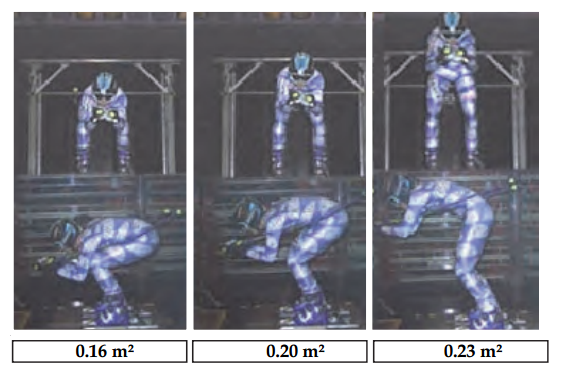
\includegraphics{airDrag}
\end{figure}

%TODO biblio link do badan
Na grafice widzimy warto�� wsp�czynnika $A$ w zale�no�ci od pozycji narciarza. Grafika pochodzi z bada� prowadzonych w tunelu aerodynamicznym IAT we Francji, przez Caroline Barelle z National Technical University of Athens z Grecji.

Pozycja narciarza ma znacz�cy wp�yw na warto�� wsp�czynnika $A$. Przyj�cie pozycji zjazdowej redukuje w stosunku do pozycji podniesionej, warto�� wsp�czynnika nawet o jedn� trzeci�. Warto nadmieni� r�wnie�, �e narciarze, nawet na amatorskich zawodach ubrani s� w specjalne kombinezony tzw. \textit{gumy narciarskie}. Kombinezony te s� jednocz�ciowe i �ci�le przylegaj� do cia�a. Nie posiadaj� �adnych odstaj�cych element�w, czasami zawieraj� tylko wewn�trzne ochraniacze w miejscach w kt�rych narciarz uderza przy ka�dym skr�cie cia�em w tyczk�. Powodem dla kt�rego str�j ten jest tak popularny r�wnie� w amatorskim sporcie jest fakt, �e znacz�co zmniejsza op�r powietrza, w stosunku do klasycznego stroju narciarskiego i potrafi na kilkudziesi�ciu sekundowej trasie, gdzie liczy si� ka�da setna sekundy, redukowa� czas przejazdu nawet o dziesi�tne cz�ci sekundy.

\subsubsection{Interakcje miedzy �niegiem a nartami}
\label{sec:interakcje}
To, �e narty �lizgaj� si� na �niegu zawdzi�czamy skomplikowanej fizyce interakcji mi�dzy powierzchni� narty a �niegiem czy lodem. Ilo�� czynnik�w jakie wp�ywaj� na jako�� tej interakcji jest bardzo du�a, a z po�r�d nich warto wymieni�:

\begin{itemize}
\item materia� wykonania �lizgu narty
\item rodzaj, jako��, spos�b nak�adania i kolejno�� nak�adania smar�w na �lizg narty
\item g�adko�� �lizgu narty
\item rodzaj i pochodzenie �niegu (naturalne/sztuczne)
\item temperatura i stopie� zanieczyszczenia �niegu
\item k�t nachylenia mi�dzy �lizgiem a pod�o�em
\end{itemize}


Jest jeszcze jeden czynnik wp�ywaj�cy na t� interakcj�, tzw. \textit{water suction} (w wolnym t�umaczeniu zasysanie wody). W temperaturze powy�ej -3 stopni Celsjusza, ciep�o powstaj�ce na skutek tarcia, topi cienk� warstw� �niegu pod nartami. Aby zredukowa� ten negatywnie wp�ywaj�cy na po�lizg efekt, �lizg narty ma perforowan� struktur�, kt�r� nale�y zachowywa� i odkrywa� po ka�dym smarowaniu, aby odprowadza� wod�. 


%TODO biblio Skiwaxes
Wed�ug bada� przeprowadzonych przez Chris'a Talbot'a z European Space Agency \cite{Skiwaxes}, tarcie o �nieg ma du�o wi�kszy wp�yw na czas przejazdu ni� si�y tarcia powietrza.

\subsubsection{Tarcie kinetyczne}
\label{sec:tarcieKinetyczne}
Tarcie kinetyczne ma du�o wi�ksze znaczenie ni� tarcie statyczne poniewa� determinuje jak du�a si�a musi dzia�a�, �eby zachowa� po��dan� pr�dko�� podczas zjazdu. Wsp�czynnik tarcia kinetycznego mi�dzy �niegiem a nasmarowanymi nartami wynosi �rednio 0.05. Wsp�czynnik ten jednak mo�e si� znacz�co zmienia� i w zale�no�ci od rodzaju smar�w, sposobu smarowania oraz jako�ci �niegu wynosi mi�dzy 0.001 a 0.3. R�nica w warto�ciach wsp�czynnik�w ma prze�o�enie w cenach smar�w, kt�re na warto�ci tych wsp�czynnik�w wp�ywaj�. Ju� na amatorskich zawodach, mo�na zaobserwowa� staranne przygotowanie �lizg�w przed ka�dym zjazdem i u�ywanie smar�w, kt�rych cena wynosi nawet kilkaset z�otych, a kt�re s� zu�ywane w ci�gu jednego sezonu start�w.  


%---------------------------------------------------------------------------

%TODO FIXME Anka czy tu co� piszemy?
\section{Metody numeryczne rozwi�zywania r�wna� r�niczkowych}
\label{sec:numeryka}


%---------------------------------------------------------------------------

\section{Optymalizacja}
\label{sec:optymalizacja}

W tym podrozdziale opisane s� metody optymalizacji u�yte w zaproponowanym rozwi�zaniu, czyli algorytm ewolucyjny oraz algorytm optymalizacji lokalnej - Hill climbing.

% czym jest optymalizacja
Zadaniem optymalizacji jest przeszukanie przestrzeni rozwi�za� w celu znalezienia najlepszego. Zatem, dana jest funkcja, nazywan� funkcj� celu, kt�ra ka�demu punktowi reprezentuj�cemu rozwi�zanie problemu przypisuje jak�� warto�� oceniaj�c� jego jako��. W�r�d wszystkich rozwi�za� poszukujemy takiego, dla kt�rego warto�� tej funkcji b�dzie jak najmniejsza (b�d� jak najwi�ksza) - najlepsza z naszego punktu widzenia. Trudno�� w znalezieniu takiego rozwi�zania zale�y od charakteru funkcji celu, a czasem tak�e od nieznajomo�ci jej analitycznej postaci.

%TODO biblio Algorytmy genetyczne i cos?
\subsubsection{Optymalizacja lokalna i globalna}
W przypadku funkcji z jednym optimum do znalezienia najlepszego rozwi�zania wystarczy przeszukiwanie lokalne. Polega ono na iteracyjnym sprawdzaniu rozwi�za� w najbli�szej przestrzeni i wprowadzaniu lokalnych zmian, aby w ko�cu znale�� rozwi�zanie najlepsze w okolicy tzw. optimum lokalne. Je�li wiemy, �e istnieje tylko jedno takie optimum, mo�emy mie� pewno��, �e znalezione rozwi�zanie jest najlepszym w ca�ej przestrzeni rozwi�za�. Przyk�adami optymalizacji lokalnych s�:
\begin{itemize}
\item hill climbing
\item przeszukiwanie tabu
\end{itemize}

Je�li natomiast funkcja celu posiada wiele optim�w lokalnych (tzw. funkcja wielomodalna) to optymalizacj� nazywamy optymalizacj� globaln�. Je�li zadanie jest ci�g�e, a wi�c niemo�liwe jest przeszukanie ca�ej przestrzeni rozwi�za�, nigdy nie mo�emy by� pewni, �e zastosowany algorytm optymalizacji da nam rozwi�zanie najlepsze - by� mo�e b�dzie to tylko minimum lokalne, a nie globalne. Nie maj�c takiej pewno�ci nie wiemy kiedy nale�y zatrzyma� algorytm. Z tego powodu stosuje si� parametr steruj�cy czasem trwania oblicze� - kosztem mniejszej pewno�ci co do poprawno�ci rozwi�zania mo�emy otrzyma� kr�tszy czas optymalizacji i odwrotnie.

\subsection{Algorytm ewolucyjny}
\label{sec:ewolucyjny}
Algorytm ewolucyjny jest przyk�adem algorytmu optymalizacyjnego, przeszukuj�cego przestrze� rozwi�za� w celu znalezienia najlepszego rozwi�zania problemu. Algorytm ten oparty jest na obserwacjach �rodowiska i przystosowywania si� organizm�w do jego warunk�w. Wiele termin�w zapo�yczonych jest zatem z genetyki.

Podstaw� ca�ego algorytmu jest populacja osobnik�w, z kt�rych ka�dy reprezentuje inne rozwi�zanie problemu. Populacja ta zmienia si� wraz z dzia�aniem algorytmu. Ewolucja zak�ada, �e populacja b�dzie si� sk�ada� z coraz lepiej przystosowanych osobnik�w. Przystosowanie to jest obliczane za pomoc� wcze�niej okre�lonej funkcji oceniaj�cej jako�� danego osobnika, czyli tak naprawd� wyznaczenie jak dobre jest rozwi�zanie reprezentowane przez niego. Przystosowanie jest warto�ci� liczbow� obliczon� za pomoc� tej funkcji przystosowania.\\
Funkcja przystosowania okre�la warto�� przystosowania osobnika na podstawie jego fenotypu, kt�ry jest tworzony z genotypu. Genotyp okre�la zestaw cech danego osobnika i sk�ada si� z chromosom�w (najcz�ciej z jednego). Natomiast ka�dy z chromosom�w sk�ada si� z elementarnych jednostek - gen�w.\\

\subsubsection{Schemat dzia�a algorytmu ewolucyjnego}
Algorytm ewolucyjny rozpoczyna si� poprzez wygenerowanie populacji bazowej oraz obliczenie przystosowania jej osobnik�w. Przewa�nie osobniki te generowane s� ca�kowicie losowo, ale mo�na tak�e wprowadzi� konkretne osobniki np. o znanym dobrym przystosowaniu do �rodowiska.

G��wna cz�� algorytmu opiera si� na powtarzaniu p�tli, w kt�rej wykonywane s� kolejno:

\begin{itemize}
\item reprodukcja
\item operacje genetyczne
\item ocena
\item sukcesja
\end{itemize}

Cz�sto reprodukcj� i sukcesj� ��czy si� pod nazw� selekcja.

Reprodukcja powoduje powielenie losowo wybranych osobnik�w z populacji. Prawdopodobie�stwo wybrania osobnika do powielenia najcz�ciej jest proporcjonalne do jego przystosowania. Mo�e si� zdarzy�, �e dany osobnik zostanie wybrany wi�cej ni� raz, a tak�e, �e nie zostanie wybrany ani razu.\\
Nast�pnie na tych kopiach przeprowadzane s� operacje genetyczne powoduj�ce zmiany w genotypie osobnik�w. Wyr�niamy dwie podstawowe operacje:

\begin{itemize}
\item mutacja
\item krzy�owanie
\end{itemize}

Zadaniem mutacji jest losowe zmodyfikowanie gen�w w genotypie.\\
Krzy�owanie, zwane tak�e rekombinacj� (ang. \textit{crossover}), dzia�a na co najmniej dw�ch osobnikach i na podstawie ich genotypu tworzy jeden lub wi�cej osobnik�w potomnych. Chromosomy rodzicielskie s� mieszane w celu otrzymania nowych genotyp�w dla osobnik�w potomnych.

W wyniku operacji genetycznych powstaj� nowe osobniki, kt�re wchodz� w sk�ad populacji potomnej. Ka�dy z tych osobnik�w jest oceniany za pomoc� funkcji przystosowania. Por�wnuj�c jako�� osobnik�w z populacji bazowej oraz potomnej dokonuje si� sukcesji, czyli wyboru osobnik�w z tych populacji (czasem wy��cznie z populacji potomnej) i tworzy now� populacj� bazow�.

Zako�czenie dzia�ania algorytmu przewa�nie opiera si� na badaniu funkcji przystosowania ca�ej populacji. Je�li warto�� przystosowania populacji nie jest zr�nicowana m�wimy o stagnacji algorytmu i mo�e by� to wskazaniem do zako�czenia dzia�ania algorytmu. Czasem jednak oczekuje si� a� przystosowanie to b�dzie wystarczaj�co du�e, �eby stwierdzi�, �e znalezione rozwi�zanie jest bardzo dobre. Przewa�nie jednak nie znamy nawet przybli�onej warto�ci jako�ci rozwi�zania, wi�c nie mo�emy stwierdzi� kiedy przystosowanie jest odpowiednie i czy nie mo�e si� jeszcze znacznie poprawi�.

\subsubsection{Kodowanie osobnik�w}
W przypadku algorytm�w genetycznych, b�d�cych szczeg�lnym przypadkiem algorytm�w ewolucyjnych, do kodowania osobnik�w stosuje si� kodowanie binarne chromosom�w. Pojedynczy bit reprezentuje zatem gen nale��cy do chromosomu.\\
W takim przypadku mutacja wykonywana jest na ka�dym genie osobno z pewnym prawdopodobie�stwem, je�li do niej dochodzi, zmienia si� warto�� bitu na przeciwn�. W krzy�owaniu wybiera si� dwa osobniki rodzicielskie, kt�rych chromosomy rozcinane s� na dwie cz�ci i ��czone "na krzy�". Miejsce przeci�cia jest losowane z rozk�adem r�wnomiernym.

W algorytmach ewolucyjnych porzuca si� kodowanie binarne - chromosom sk�ada si� z jednej lub wi�cej liczb stanowi�cych cechy osobnika.\\
Mutacja takiego osobnika najcz�ciej odbywa si� poprzez losow� zmian� ka�dej z warto�ci gen�w chromosomu. Do krzy�owania wybiera si� dwa osobniki, z kt�rych dla ka�dej pary odpowiadaj�cych gen�w wyci�gana jest �rednia i tak otrzymane warto�ci gen�w tworz� genotyp nowego osobnika.

\subsubsection{Typy algorytm�w ewolucyjnych}
Algorytmy ewolucyjne wywodz� si� z kilku osobnych nurt�w zajmuj�cych si� t� tematyk�, wi�c istnieje wiele podobnych schemat�w dzia�ania. Najlepiej traktowa� algorytmy ewolucyjne jako metaheurystyk� - okre�lony jest pewien szkic algorytmu, kt�ry mo�na dostosowywa� do konkretnego rozwi�zania. W tym podrozdziale opisane s� podstawowe i najbardziej popularne schematy post�powania oparte o algorytmy ewolucyjne.\\


\textbf{Prosty algorytm genetyczny}

Prosty algorytm genetyczny zosta� zaproponowany w roku 1975 przez John'a Holland'a.

Poni�ej umieszczony jest schemat tego algorytmu (\ref{alg:prostyGenetyczny}).

\begin{algorithm}
\caption{Prosty algorytm genetyczny}
\label{alg:prostyGenetyczny}
\begin{algorithmic}
\STATE	$t = 0$
\STATE	$P^0 = createInitPop() $
\WHILE {$stopCondition == false$}
\STATE	$T^t = createTempPop(P^t) $
\STATE	$T^t = crossPop(T^t) $
\STATE	$O^t = mutatePop(T^t) $
\STATE	$P^{t+1} = O^t$
\STATE	$t=t+1$
\ENDWHILE
\end{algorithmic}
\end{algorithm}


Maj�c populacj� bazow� $P^t$ dokonujemy reprodukcji tej populacji, tworz�c populacj� tymczasow� $T^t$ sk�adaj�c� si� z takiej samej liczby osobnik�w. Wybierani s� oni z prawdopodobie�stwem proporcjonalnym do ich przystosowania z populacji bazowej. Na populacji tymczasowej dokonujemy operacji genetycznych (mutacji i krzy�owania). Do krzy�owania wybierane s� roz��czne pary osobnik�w i z pewnym prawdopodobie�stwem $p_c$ zachodzi ich skrzy�owanie. Je�li dosz�o do powstania osobnik�w potomnych zast�puj� one osobniki rodzicielskie. Nast�pnie na tak otrzymanej populacji tymczasowej dochodzi do mutacji osobnik�w i otrzymania populacji potomnej $O^t$. Ta populacja staje si� w nast�pnej iteracji algorytmu now� populacj� bazow�.\\
Zatrzymanie algorytmu mo�e by� dokonane je�li np.:

\begin{itemize}
\item wykonano okre�lon� z g�ry liczb� iteracji
\item znaleziono osobnika o wystarczaj�co wysokiej warto�ci przystosowania
\end{itemize}

W tej wersji algorytmu cz�sto p�tl� algorytmu nazywa si� generacj�, a ka�d� populacj� $P^t$ w chwili t pokoleniem.\\

\textbf{Strategia (1+1)}

Strategia (1+1) jest podstawow� strategi� ewolucyjn�. W algorytmie tym mamy do czynienia z populacj� sk�adaj�c� si� tylko z jednego osobnika posiadaj�cego jeden chromosom. W ka�dej p�tli algorytmu dokonuje si� mutacji tego chromosomu, co powoduje powstanie nowego osobnika. Osobnik ten jest poddawany ocenie, a nast�pnie dokonuje si� wyboru lepszego z dw�ch istniej�cych osobnik�w i tego pozostawia w populacji.\\
W mutacji dodaje si� do ka�dego genu chromosomu losow� modyfikacj� rozk�adem normalnym:
\begin{equation}
Y^t_i = X^t_i + \sigma\xi_{N(0,1),i}
\end{equation}

Warto�� $\sigma$ b�dzie powodowa�a wi�ksze lub mniejsze zmiany w chromosomie. Je�li chcemy przeszuka� przestrze� rozwi�za�, powinni�my zwi�ksza� jej warto��, co jest po��dane zw�aszcza w pocz�tkowej fazie dzia�ania algorytmu. Natomiast, aby znale�� jak najlepsze rozwi�zanie, wiedz�c �e obecne rozwi�zanie jest ju� bardzo bliskie najlepszemu, mo�emy zmniejsza� warto�� $\sigma$ przeszukuj�c tylko najbli�sz� przestrze�.\\
Do wyznaczania $\sigma$ powsta� nast�puj�cy algorytm zwany regu�� 1/5 sukces�w:
\begin{enumerate}
\item Je�li przez kolejnych k p�tli algorytmu mutacja powoduje powstanie lepszego osobnika w wi�cej ni� 1/5 wszystkich mutacji, to zwi�kszamy $\sigma$: $\sigma' = c_i \sigma$. Warto�� $c_i$ wyznaczona empirycznie wynosi $ \frac{1}{0.82} $
\item Gdy dok�adnie 1/5 ko�czy si� sukcesem, warto�� $\sigma$ pozostaje bez zmian.
\item Je�li nie zachodzi �adne z powy�szych warto�� $\sigma$ jest zmniejszana: $\sigma' = c_d \sigma$. Gdzie $ c_d $ powinna wynosi� $ 0.82 $
\end{enumerate}

\textbf{Strategia ($\mu$ + $\lambda$)}

Strategia ($\mu$ + $\lambda$) jest rozwini�ciem strategii (1+1). $\mu$ oznacza ilo�� osobnik�w w populacji pocz�tkowej, a $\lambda$ ile osobnik�w jest reprodukowanych i poddawanych operacjom genetycznym. Dodatkowo, zamiast regu�y 1/5 sukces�w wprowadzono mechanizm samoczynnej adaptacji zasi�gu mutacji, a tak�e wprowadzono operator krzy�owania.

Oznaczenie $\mu$ + $\lambda$ oznacza, �e po wygenerowaniu populacji potomnej wybierane jest $\mu$ najlepszych osobnik�w do nowej populacji bazowej - zar�wno spo�r�d populacji potomnej, jak i starej populacji bazowej zawieraj�cych ��cznie $\mu$ + $\lambda$ osobnik�w. Algorytm \ref{alg:miPlusLambda} przedstawia schemat dzia�ania.

\begin{algorithm}
\caption{Strategia ewolucyjna (\mu + \lambda)}
\label{alg:miPlusLambda}
\begin{algorithmic}
\STATE	$t = 0$
\STATE	$P^0 = createInitPop(\mu) $
\WHILE {$stopCondition == false$}
\STATE	$T^t = createTempPop(P^t,\lambda) $
\STATE	$T^t = crossPop(T^t) $
\STATE	$O^t = mutatePop(T^t) $
\STATE	$P^{t+1} = select(O^t \cup P^t,\mu)$
\STATE	$t=t+1$
\ENDWHILE
\end{algorithmic}
\end{algorithm}


W strategii tej wa�ne jest te� kodowanie, do kt�rego dodatkowo do�o�ono r�wnie� chromosom przechowuj�cy wektor $\sigma$ zawieraj�cy warto�ci odchyle� standardowych, kt�re wykorzystuje si� w trakcie mutacji.\\
Po wylosowaniu warto�ci zmiennej losowej o rozk�adzie normalnym ($\xi_{N(0,1)}$) dla ka�dego elementu wektora $\sigma$ losujemy jeszcze jedn� zmienn� losow� o rozk�adzie normalnym ($\xi_{N(0,1),i}$) i obliczamy nowe warto�ci odchyle� z wektora $\sigma$:

\begin{equation}
\sigma'_i = \sigma_i e^{(\tau'\xi_{N(0,1)} + \tau\xi_{N(0,1),i})}
\end{equation}


Gdzie $\tau$ oraz $\tau'$ s� parametrami algorytmu, a ich warto�ci powinny wynosi�:
\begin{equation}
\tau = \frac{K}{\sqrt{2n}}
\end{equation}

\begin{equation}
\tau' = \frac{K}{\sqrt{2\sqrt{n}}}
\end{equation}

%TODO biblio Schwefel(1995) (http://ls11-www.cs.uni-dortmund.de/people/rudolph/publications/papers/gra.pdf)
gdzie:
K - sta�a, najcz�ciej stosuje si� warto�� 1
n - wymiarowo�� zadania

Maj�c dane nowe warto�ci odchyle� standardowych mo�emy obliczy� nowe warto�ci gen�w korzystaj�c ze wzoru:

\begin{equation}
X'_i = X_i + \sigma'_i\xi_{N(0,1),i}
\end{equation}
gdzie $\xi_{N(0,1),i}$ jest now� losow� warto�ci�.

Algorytm ewolucyjny wybiera osobniki lepiej przystosowane, a wi�c te, kt�re posiadaj� tak�e lepsze warto�ci odchyle� standardowych. Powoduje to naturaln� selekcj�, doprowadzaj�c� do samoczynnej adaptacji odchyle� standardowych stosowanych w trakcie mutacji.

Krzy�owanie wyst�puje w tym algorytmie pod nazw� rekombinacja. Najcz�ciej sprowadza si� do u�rednienia lub wymianie warto�ci wektor�w, tak�e wektora $\sigma$.

\textbf{Strategia ($\mu$, $\lambda$)}
Strategia ($\mu$ + $\lambda$) posiada pewne wady, kt�re postanowiono spr�bowa� wyeliminowa� za pomoc� nowej strategii ($\mu$, $\lambda$). Poprzedni algorytm sprawia problemy je�li w populacji pojawia si� osobnik o wysokiej warto�ci przystosowania, ale posiadaj�cy zbyt du�e (albo zbyt ma�e) warto�ci odchyle� standardowych. Usuni�cie takiego osobnika z populacji cz�sto nie jest procesem kr�tkotrwa�ym, gdy� wp�ywa on na powstaj�ce potomstwo, przekazuj�c mu podobne do jego, nieodpowiednie warto�ci odchyle�.\\
W nowej strategii wprowadzono zmian�, kt�ra powoduje, �e osobniki rodzicielskie nie s� nigdy brane do kolejnej populacji bazowej. Podczas selekcji korzysta si� zatem tylko z powsta�ej populacji potomnej, z niej wybieraj�c osobniki do populacji bazowej w kolejnej iteracji. Algorytm \ref{alg:miLambda} prezentuje kolejne kroki schematu tego algorytmu.

\begin{algorithm}
\caption{Strategia ewolucyjna (\mu, \lambda)}
\label{alg:miLambda}
\begin{algorithmic}
\STATE	$t = 0$
\STATE	$P^0 = createInitPop(\mu) $
\WHILE {$stopCondition == false$}
\STATE	$T^t = createTempPop(P^t,\lambda) $
\STATE	$T^t = crossPop(T^t) $
\STATE	$O^t = mutatePop(T^t) $
\STATE	$P^{t+1} = select(O^t,\mu)$
\STATE	$t=t+1$
\ENDWHILE
\end{algorithmic}
\end{algorithm}

\subsection{Hill Climbing}
\label{sec:hill}
%TODO biblio ksiazka Stuart Russell, Peter Norvig - Artificial Inteligence A Modern Approach

Algorytm Hill Climbing jest jedn� z metod przeszukiwania lokalnego. W ka�dej iteracji zmieniaj�c warto�� rozwi�zania w jednym z wymiar�w sprawdzana jest warto�� funkcji celu dla nowego rozwi�zania i je�li warto�� ta jest lepsza od dotychczas najlepszej znalezionej, zapami�tujemy zmienione rozwi�zanie. Dop�ki zmiany powoduj� popraw� rozwi�zania, algorytm nie jest zatrzymywany. Na ko�cu wiemy, �e znalezione rozwi�zanie jest rozwi�zaniem lokalnie optymalnym.\\
Przeszukiwanie przestrzeni dyskretnej sprowadza si� do sprawdzania rozwi�za� najbli�szych obecnemu i wybieranie tego rozwi�zania, kt�rego warto�� obliczona za pomoc� funkcji celu jest najlepsza. Je�li w�r�d s�siad�w nie ma ju� lepszego rozwi�zania, mo�emy zako�czy� przeszukiwanie. Pseudokod algorytmu przedstawiony jest poni�ej (Algorytm \ref{alg:hillClimbDiscrete}).\\

\begin{algorithm}
\caption{Hill Climbing w przestrzeni dyskretnej}
\label{alg:hillClimbDiscrete}
\begin{algorithmic}
\STATE $current = startPoint$
\STATE $foundBetter = true $
\WHILE {$ foundBetter == true $}
  \STATE $ foundBetter = false $
  \STATE $ neighbours = getNeighbours(current) $
  \FORALL {$neighbour$ $in$ $neighbours$}
    \IF {$ neighbour.isBetterThan(current) $}
      \STATE $ current = neighbour $
      \STATE $ foundBetter = true $
    \ENDIF
  \ENDFOR
\ENDWHILE
\end{algorithmic}
\end{algorithm}


W przestrzeni ci�g�ej konieczne jest dobranie kroku, kt�ry wyznacza punkty przeszukiwane w okolicy w trakcie ka�dej iteracji. Dodatkowo wykorzystywane jest tzw. przyspieszenie (ang. \textit{acceleration}), kt�re wyznacza pi�ciu mo�liwych kandydat�w na lepsze rozwi�zania. Najcz�ciej przyspieszenie to wynosi 1.2, a warto�� kroku jest osobna dla ka�dej zmiennej rozwi�zania i cz�sto wynosi na pocz�tku 1. Zatem za ka�dym razem obliczane s� nast�puj�ce wsp�czynniki: -acceleration, -1/acceleration, 0, 1/acceleration, acceleration. Nast�pnie wsp�czynniki mno�one s� przez krok (step) i dodawane do obecnie analizowanej zmiennej i wybierane jest najlepsze z pi�ciu rozwi�za�. Warto�� kroku jest indywidualna dla ka�dej zmiennej. Po wybraniu najlepszego rozwi�zania uaktualniana jest warto�� tego kroku - krok mno�ony jest przez odpowiedni wsp�czynnik, ten kt�ry by� dobrany wcze�niej do znalezienia tego najlepszego rozwi�zania. Algorytm zatrzymywany jest je�li zmiana �adnej ze zmiennych nie przynosi ju� poprawy rozwi�zania, czasem r�wnie� je�li ta zmiana jest ju� bardzo ma�a - wprowadzany jest parametr $\epsilon$ wyznaczaj�cy t� r�nic�. Pseudokod algorytmu przedstawiony jest na kolejnej stronie (Algorytm \ref{alg:hillClimbCont}).


\begin{algorithm}
\caption{Hill Climbing w przestrzeni ci�g�ej}
\label{alg:hillClimbCont}
\begin{algorithmic}
\STATE $ currentResult = startPoint$
\STATE $ steps = initialSteps $ \COMMENT {for each dimension of the solution}
\STATE $ candidates = [-acc, -\frac{1}{acc}, 0, \frac{1}{acc}, acc] $
\STATE $ currentValue = currentResult.getValue() $
\STATE $ beforeValue = MAX\_VALUE $
\STATE $ \epsilon = EPSILON $
\WHILE {$ beforeValue - currentValue > \epsilon $}
  \STATE $ beforeValue = currentValue $
  \FOR {$i$ $in$ $dimensions$}
    \STATE $ bestIndex = -1 $
	\STATE $ bestScore = MAX\_VALUE $\
	\FOR {$j$ $in$ $candidatesNrs$} 
	  \STATE $ currentResult[i] = currentResult[i] + stepSize[i] * candidates[j] $
	  \STATE $ tempValue = currentResult.getValue() $
	  \STATE $ currentResult[i] = currentResult[i] - stepSize[i] * candidates[j] $
	  \IF {$tempValue.isBetterThan(bestScore)$}
	    \STATE $ bestScore = tempValue $
	    \STATE $ bestIndex = j $
	  \ENDIF
	\ENDFOR
	\IF {$ candidates[bestIndex]!=0 $}
   	  \STATE $ currentResult[i] = currentResult[i] + stepSize[i] * candidates[bestIndex] $
	  \STATE $ stepSize[i] = stepSize[i] * candidates[bestIndex] $    	  \COMMENT {accelerate}
	\ENDIF
  \ENDFOR
  \STATE $ currentValue = bestScore $
\ENDWHILE
\end{algorithmic}
\end{algorithm}

%---------------------------------------------------------------------------

%TODO biblio
\section{Volunteer Computing}
\label{volunteerComputing}

Volunteer Computing to nieformalny kontrakt, w kt�rym zwykli ludzie czy te� organizacje, nazywani dalej ochotnikami, dobrowolnie udost�pniaj� swoje zasoby obliczeniowe, by uruchamia� na nich obliczenia zwi�zane z r�norakimi projektami. S� to przewa�nie projekty naukowe, kt�rych celem jest rozwi�zanie problem�w i zada� matematycznych czy te� problem�w dotykaj�cych ludzko��, lub d���cych do lepszego poznania �wiata i wszech�wiata. Dzi�ki platformom umo�liwiaj�cym Volunteer Computing, ka�dy cz�owiek mo�e w niewielkim stopniu mie� wk�ad w rozwi�zywanie tych problem�w.

Procesory w komputerach osobistych sp�dzaj� oko�o 80 procent czasu nie robi�c nic. R�wnocze�nie wiele naukowych problem�w zwi�zanych na przyk�ad z modelowaniem zmian klimatu potrzebuje ogromnych zasob�w obliczeniowych. U�ywanie do tego celu superkomputer�w jest bardzo drogie. Po��czenie tych fakt�w doprowadzi�o do stworzenia konceptu, by u�ywa� do tych oblicze� zasob�w zwyk�ych ludzi, kt�rzy chc� si� �wiadomie nimi dzieli�. Obecne do�wiadczenia wskazuj�, �e wydajno�� systemu dla pojedynczo prowadzonego projektu opartego o Volunteer Computing jest por�wnywalna do tego, gdyby projekt prowadzony by� przy wsparciu jednego z topowych superkomputer�w z listy TOP500.

Ochotnicy to osoby prywatne albo instytucje takie jak szko�y czy uniwersytety. Ochotnicy przewa�nie pozostaj� anonimowi, cho� w niekt�rych projektach wymagane jest dostarczenie podstawowych danych kontaktowych jak np. adresu email. W wypadku celowego dostarczania b��dnych wynik�w przez ochotnika, utrudnione jest jego dyscyplinowanie czy te� wy��czenie z projektu. Ochotnicy nie s� wynagradzani finansowo za uczestnictwo w projekcie. 

Organizacja czy osoba chc�ca wykorzysta� model Volunteer computing do swoich projekt�w, musi by� jednostk� zaufan� dla ochotnik�w realizuj�cych obliczenia. Wynika to z prostego faktu, �e ochotnicy decyduj� si�, wed�ug standardowego modelu computing, na zainstalowanie aplikacji dostarczanej przez dawc� zada� obliczeniowych. Osoba instaluj�ca aplikacj� musi ufa�, �e nie uszkodzi ona jej komputera, ani te� nie b�dzie wykorzystywa� jej zasob�w w spos�b niezgodny z zapewnieniami zleceniodawcy oblicze�. Zleceniobiorca oblicze� ma te� prawo oczekiwa�, �e aplikacja, zosta�a napisana przestrzegaj�c dobrych praktyk bezpiecze�stwa, gdy� jako, �e aplikacja ta ��czy si� z internetem i potencjalnie jest zainstalowana na du�ej ilo�ci maszyn, jest wi�c atrakcyjnym celem atak�w zmierzaj�cych do przej�cia tych maszyn do niezgodnych z prawem cel�w przez haker�w. 

Przewa�nie model komunikacyjny systemu Volunteer Computing uwzgl�dnia tylko komunikacj� poszczeg�lnych klient�w z centralnym serwerem i nie zak�ada bezpo�redniej komunikacji mi�dzy klientami.

Volunteer Computing pierwotnie zak�ada�, �e obliczenia s� wykonywane na zwyk�ych komputerach osobistych (PC). Ilo�� komputer�w tego typu jest niepor�wnywalnie wi�ksza ni� ilo�� wyspecjalizowanych komputer�w o du�ej mocy obliczeniowej i jest szacowana na ponad miliard. Dodatkowo, z przyczyn ekonomicznych, na rozw�j tych maszyn producenci sprz�tu przeznaczaj� najwi�ksze fundusze, wi�c ich moc i zdolno�ci obliczeniowe stale rosn�. 

Wa�nym aspektem, kt�ry istotnie wp�ywa na stosowanie modelu w praktyce, jest koszt prowadzenia oblicze�. Model zak�ada, �e do��czanie si� do oblicze� jest dobrowolne i nie dostaje si� za uczestnictwo w projekcie wynagrodzenia. Dzi�ki temu, projekty, kt�re maj� poparcie i akceptacj� spo�eczn� mog� liczy� na darmowe moce obliczeniowe udost�pnione przez zwyk�ych ludzi.

Na ten model mo�na patrzy� tak�e w kategoriach edukacyjnych. Podczas gdy ochotnik przyst�puje do projektu i udost�pnia swoje moce obliczeniowe, mo�na wykorzysta� jego potencjalne zainteresowanie rozwi�zywanym problemem i za pomoc� przyst�pnych wizualizacji przedstawi� mu sedno rozwi�zywanego zadania, nakre�li� mu problem z r�nych perspektyw i pokaza� mu do czego potencjalnie zmierzaj� obliczenia. Po��czenie atrakcyjnej formy t�umaczenia rozwi�zywanych problem�w z potencja�em portali spo�eczno�ciowych i popularno�ci ciekawego materia�u mo�na uzyska� daleko id�cy efekt propagacji i pod��czaniu si� do oblicze� coraz wi�kszej ilo�ci os�b.

%TODO biblio
\section{Web Workers}
\label{webWorkers}

Przeprowadzanie intensywnych oblicze� w przegl�darkach internetowych nie by�o mo�liwe do czasu wprowadzenia przez grup� WHATWG (Web Hypertext Application Technology Working Group) specyfikacji Web Worker. Ograniczenie wynika�o z faktu, �e j�zyk w kt�rym wykonywane s� skrypty poprzez silniki przegl�darki to Java Script. Java Script to �rodowisko jednow�tkowe, wi�c nic nie mo�e by� wykonywane r�wnolegle. Zlecaj�c wi�c skryptowi intensywne obliczenia, na ich ca�y czas UI strony by�by nieresponsywny, co jest nie do przyj�cia dla cz�owieka obs�uguj�cego stron� internetow�. Przegl�darki broni� u�ytkownika przed takim zachowaniem skrypt�w na stronie i czasami zdarza si� jeszcze zobaczy� okno z ostrze�eniem, �e skrypt przesta� odpowiada� i mo�liwo�ci� manualnego zatrzymania skryptu.

Web Workers definiuje API do tworzenia osobnych proces�w w tle. Worker'y wykorzystuj� do komunikacji z w�tkiem g��wnym klasyczny model przekazywania wiadomo�ci. Nowoczesne przegl�darki umo�liwiaj� przekazywanie zar�wno tekstu jak i obiekt�w zserializowanych w formacie JSON. Nale�y zwr�ci� uwag�, �e obiekty te nie s� wsp�dzielone, ale w pe�ni kopiowane. 

Web Worker'y nie maj� dost�pu do struktury DOM, obiektu \textit{window} ani \textit{document}. Zewn�trzne skrypty wykorzystywane przez worker'a musz� by� serwowane z tej samej domeny co kod worker'a.

Wed�ug specyfikacji, stworzonej przez WHATWG, Web Workery powinny by� u�ywane do zada� trwaj�cych d�u�szy czas, maj�cych du�y narzut startowy i spory narzut pami�ciowy. Nie jest wi�c odpowiednim tworzenie bardzo wielu worker'�w zajmuj�cych si� obliczeniami trwaj�cymi marginalny czas, gdy� sam narzut na stworzenie przez przegl�dark� osobnego procesu mo�e by� zbyt du�y, by uzasadni� jego u�ycie.

\chapter{Wprowadzenie teoretyczne i istniej�ce rozwi�zania - Volunteer Computing}
\label{cha:rozwiazania}

W rozdziale tym przedstawimy istniej�ce rozwi�zania zar�wno architektoniczne, kt�re umo�liwiaj� rozproszone obliczenia w modelu Volunteer Computing, jak i rozwi�zania dotykaj�ce problemu zwi�zanego z poszukiwaniem optymalnej trasy narciarza na slalomie. 

%---------------------------------------------------------------------------
\section{Volunteer Computing}
\label{volunteerComputing}

%TODO Ania wstaw prosze odno�nik do pozycji VolunteerIntro z biblio
Volunteer Computing to model obliczeniowy, w kt�rym zwykli ludzie czy te� organizacje, nazywani dalej ochotnikami, dobrowolnie udost�pniaj� swoje zasoby obliczeniowe, by uruchamia� na nich obliczenia zwi�zane z r�norakimi projektami. S� to przewa�nie projekty naukowe, kt�rych celem jest rozwi�zanie problem�w i zada� matematycznych czy te� problem�w dotykaj�cych ludzko��, lub d���cych do lepszego poznania �wiata i wszech�wiata. Dzi�ki platformom u�ywaj�cym modelu Volunteer Computing, ka�dy cz�owiek mo�e mie� wk�ad w rozwi�zywanie tych problem�w.

Procesory w komputerach osobistych s� bezczynne przez oko�o 80 procent czasu. R�wnocze�nie wiele naukowych problem�w zwi�zanych na przyk�ad z modelowaniem zmian klimatu potrzebuje ogromnych zasob�w obliczeniowych. U�ywanie do tego celu superkomputer�w jest bardzo drogie. Po��czenie tych fakt�w doprowadzi�o do stworzenia modelu, wykorzystuj�cego zasoby obliczeniowe ochotnik�w, kt�rzy chc� si� nimi �wiadomie dzieli�. 

Moc obliczeniowa najmocniejszego superkomputera z listy TOP500, na listopad 2013, jest tego samego rz�du co moc obliczeniowa generowana przez ochotnik�w u�ywaj�cych platformy do Volunteer Computingu - BOINC opisanej w rozdziale \pageref{sec:BOINC}, na dzie� 26 Grudnia 2013. Moc ta wynosi oko�o 9 Peta flops�w dla BOINC i 33 Peta flops�w dla National Super Computer Center in Guangzhou, China z listy TOP500. Flops to jednostka wyra�aj�ca moc obliczeniow� i wskazuj�ca ile operacji zmiennoprzecinkowych na jedn� sekund� komputer mo�e wykonywa�. Moc rz�du 9 peta flops to ${9}*{10}^{15}$ operacji zmiennoprzecinkowych na sekund�


\begin{figure}[h]
\centering
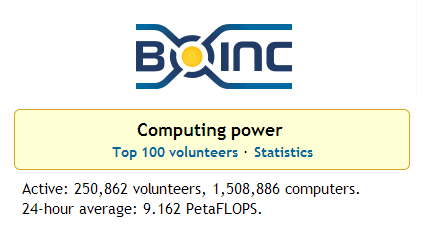
\includegraphics[width=200px]{boinc-26-12}
\caption{Zrzut ekranu ze strony internetowej https://boinc.berkeley.edu/, z dnia 26/12/2013 pokazuj�cy �redni� moc obliczeniow� systemu z ostatnich 24 godzin.}
\label{fig:boinc-26-12}
\end{figure}


\begin{figure}[h]
\centering
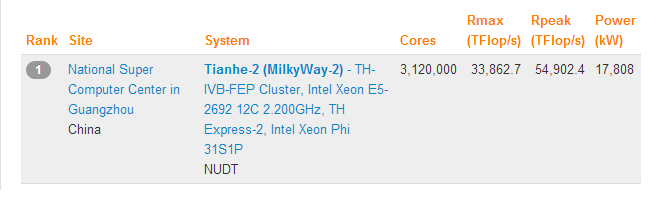
\includegraphics[width=300px]{top500-november2013}
\caption{Zrzut ekranu ze strony http://www.top500.org/lists/2013/11/ pokazuj�cu pierwsze miejsce na li�cie TOP500 z listopada 2013 roku.}
\label{fig:top500-november2013}
\end{figure}


Ochotnicy to osoby prywatne albo instytucje takie jak szko�y czy uniwersytety. Ochotnicy przewa�nie pozostaj� anonimowi, cho� w niekt�rych projektach wymagane jest dostarczenie podstawowych danych kontaktowych jak np. adresu email. Czasem zdarza si�, �e ochotnicy z premedytacj� przek�amuj� wysy�ane do centralnego serwera wyniki swoich oblicze�. Z uwagi na anonimowo�� ochotnik�w, utrudnione jest w takich przypadkach ich dyscyplinowanie czy te� wy��czenie z projektu. Ochotnicy nie s� wynagradzani finansowo za uczestnictwo w projekcie. 

Organizacja czy osoba chc�ca wykorzysta� model Volunteer computing do swoich projekt�w, musi by� jednostk� zaufan� dla ochotnik�w realizuj�cych obliczenia. Wynika to z prostego faktu, �e ochotnicy decyduj� si�, wed�ug standardowego modelu obliczeniowego, na zainstalowanie aplikacji dostarczanej przez dostarczyciela zada� obliczeniowych. Osoba instaluj�ca aplikacj� musi ufa�, �e nie uszkodzi ona jej komputera, ani te� nie b�dzie wykorzystywa� jej zasob�w w spos�b niezgodny z zapewnieniami zleceniodawcy oblicze�. Ma te� prawo oczekiwa�, �e aplikacja, zosta�a napisana przestrzegaj�c dobrych praktyk bezpiecze�stwa, gdy� jako, �e aplikacja ta ��czy si� z internetem i potencjalnie jest zainstalowana na du�ej ilo�ci maszyn, jest wi�c atrakcyjnym celem atak�w zmierzaj�cych do przej�cia tych maszyn przez haker�w, do niezgodnych z prawem cel�w. 

Przewa�nie model komunikacyjny systemu Volunteer Computing uwzgl�dnia tylko komunikacj� poszczeg�lnych klient�w z centralnym serwerem i nie zak�ada bezpo�redniej komunikacji mi�dzy klientami.
%TODO Ania wstaw prosz� odno�nik do VolunteerIntro  - ROmek chcia�

Volunteer Computing pierwotnie zak�ada�, �e obliczenia s� wykonywane na zwyk�ych komputerach osobistych (PC). Ilo�� komputer�w tego typu jest niepor�wnywalnie wi�ksza ni� ilo�� wyspecjalizowanych komputer�w o du�ej mocy obliczeniowej i jest szacowana na ponad miliard. Dodatkowo, z przyczyn ekonomicznych, na rozw�j tych maszyn producenci sprz�tu przeznaczaj� najwi�ksze fundusze, wi�c ich moc i zdolno�ci obliczeniowe stale rosn�. 

Wa�nym aspektem, kt�ry istotnie wp�ywa na stosowanie modelu w praktyce, jest koszt prowadzenia oblicze�. Model zak�ada, �e do��czanie si� do oblicze� jest dobrowolne i nie dostaje si� za uczestnictwo w projekcie wynagrodzenia. Dzi�ki temu, projekty, kt�re maj� poparcie i akceptacj� spo�eczn� mog� liczy� na darmowe moce obliczeniowe udost�pnione przez zwyk�ych ludzi.

Na ten model mo�na patrzy� tak�e w kategoriach edukacyjnych. Podczas gdy ochotnik przyst�puje do projektu i udost�pnia swoje moce obliczeniowe, mo�na wykorzysta� jego potencjalne zainteresowanie rozwi�zywanym problemem i za pomoc� przyst�pnych wizualizacji przedstawi� mu sedno rozwi�zywanego zadania, nakre�li� mu problem z r�nych perspektyw i pokaza� mu do czego potencjalnie zmierzaj� obliczenia. Po��czenie atrakcyjnej formy t�umaczenia rozwi�zywanych problem�w z potencja�em portali spo�eczno�ciowych i popularno�ci ciekawego materia�u mo�na uzyska� daleko id�cy efekt propagacji i pod��czaniu si� do oblicze� coraz wi�kszej ilo�ci os�b.

\section{Web Workers}
\label{webWorkers}

%TODO Ania wstaw prosz� odno�nik do pozycji WebWorkersSpec z biblio
Przeprowadzanie intensywnych oblicze� w przegl�darkach internetowych nie by�o mo�liwe do czasu wprowadzenia przez grup� WHATWG (Web Hypertext Application Technology Working Group) specyfikacji Web Worker. Ograniczenie wynika�o z faktu, �e j�zyk w kt�rym wykonywane s� skrypty poprzez silniki przegl�darki to Java Script. Java Script to �rodowisko jednow�tkowe, wi�c nic nie mo�e by� wykonywane r�wnolegle. Zlecaj�c wi�c skryptowi intensywne obliczenia, na ich ca�y czas UI strony by�by nieresponsywny, co jest nie do przyj�cia dla cz�owieka obs�uguj�cego stron� internetow�. Przegl�darki broni� u�ytkownika przed takim zachowaniem skrypt�w na stronie i czasami zdarza si� jeszcze zobaczy� okno z ostrze�eniem, �e skrypt przesta� odpowiada� i mo�liwo�ci� manualnego zatrzymania skryptu.

Web Workers definiuje API do tworzenia osobnych proces�w w tle. Worker'y wykorzystuj� do komunikacji z w�tkiem g��wnym klasyczny model przekazywania wiadomo�ci. Nowoczesne przegl�darki umo�liwiaj� przekazywanie zar�wno tekstu jak i obiekt�w zserializowanych w formacie JSON. Nale�y zwr�ci� uwag�, �e obiekty te nie s� wsp�dzielone, ale w pe�ni kopiowane. 

Web Worker'y nie maj� dost�pu do struktury DOM, obiektu \textit{window} ani \textit{document}. Zewn�trzne skrypty wykorzystywane przez worker'a musz� by� serwowane z tej samej domeny co kod worker'a.

Wed�ug specyfikacji, stworzonej przez WHATWG, Web Workery powinny by� u�ywane do zada� trwaj�cych d�u�szy czas, maj�cych du�y narzut startowy i spory narzut pami�ciowy. Nie jest wi�c odpowiednim tworzenie bardzo wielu worker'�w zajmuj�cych si� obliczeniami trwaj�cymi marginalny czas, gdy� sam narzut na stworzenie przez przegl�dark� osobnego procesu mo�e by� zbyt du�y, by uzasadni� jego u�ycie.


\section{Platformy do Volunteer Computing}
\label{sec:platformyDoVolunteerComputing}

W klasycznym modelu, architektura umo�liwiaj�ca prowadzenie oblicze� w modelu Volunteer Computing sk�ada�a si� z aplikacji klienckich, kt�re musz� by� pobrane oraz zainstalowane na  komputerze typu PC, oraz serwera, kt�ry zarz�dza wysy�aniem zada� i odbieraniem rozwi�za�. 

Konieczno�� pobierania i instalowania aplikacji na urz�dzeniu implikuje wym�g tworzenia i utrzymywania wersji aplikacji pod ka�dy znacz�cy system operacyjny. Proces wyboru odpowiedniej kompilacji programu klienckiego oraz jego instalacji jest pierwsz� barier� jak� napotyka przeci�tna osoba chc�ca mie� sw�j wk�ad do naukowego projektu.

Zleceniodawcy oblicze�, zauwa�yli, �e na �wiecie popularno�� zdobywaj� inne od komputer�w osobistych urz�dzenia, kt�re r�wnie� dysponuj� nie wykorzystywan� moc� obliczeniow�. Konsola Play Station 3 by�a pierwszym urz�dzeniem tego typu, w��czonym do projekt�w wykorzystuj�cych Volunteer Computing. W sierpniu 2013 udost�pniono natomiast aplikacj� do naukowych projekt�w, dzi�ki kt�rej mo�na kontrybuowa� po�wi�caj�c zasoby obliczeniowe swojego urz�dzenia z systemem Android.

W ostatnich latach, mo�na zaobserwowa� trend przenoszenia oprogramowania, kt�re dotychczas zainstalowane by�o na komputerach jako natywna aplikacja, w model SAAS (Software As A Service). Programy pocztowe, funkcjonalne systemy CRM, czy odtwarzacze muzyczne coraz cz�ciej dost�pne s� za po�rednictwem przegl�darek internetowych. Taka zmiana mo�liwa by�a dzi�ki rozwojowi silnik�w Java Script we wsp�czesnych przegl�darkach, oraz implementacja w przegl�darkach zaawansowanych element�w ze specyfikacji HTML5 oraz Web Workers.

W tym rozdziale, zaprezentujemy przekr�j obecnie najbardziej znacz�cych projekt�w korzystaj�cych z modelu Voluneteer Computing oraz platform, kt�re te projekty wykorzystuj�.

\subsection{Great Internet Mersenne Prime Searchy}
\label{sec:gimps}
Pierwszym projektem wykorzystuj�cym Volunteer Computing jest rozpocz�ty na pocz�tku 1996 roku a trwaj�cy do dzi� \textit{GIMPS} (Great Internet Mersenne Prime Search), kt�rego celem jest znalezienie jak najwi�kszej ilo�ci specyficznych liczb pierwszych - tzn. Liczb Pierwszych Marsenne'a. Do tej pory kolaboracyjne wysi�ki doprowadzi�y do odnalezienia czternastu takich liczb. Moc systemu da�aby teoretycznie, wg. danych na listopad 2012 roku - 330-te miejsce w rankingu TOP500 - rankingu najmocniejszych komputer�w na �wiecie. 

System sk�ada si� z aplikacji klienckich stworzonych dla 9 platform i konfiguracji system�w. Tw�rcy zapewniaj�, �e kod programu jest wysoce zoptymalizowanym kodem asemblerowym Intela. Po uruchomieniu, program nawi�zuje kontakt z serwerem nazwanym \textit{PrimeNet}, aby otrzyma� cz�� pracy.

\textit{GIMPS} jest ciekawym projektem, kt�ry ma swoje sukcesy i skal�, co potwierdzaj� publikowane regularnie informacje o nowych znaleziskach oraz wielko�ci sieci komputer�w bior�cych udzia� w obliczeniach. Interfejs i wygoda u�ytkowania (ang. \textit{User Experience}), kt�re oferuje platforma s� jednak bardzo s�abe i archaiczne i zupe�nie nieprzystosowane do u�ytkownik�w wsp�czesnego internetu.  

\subsection{Distributed.net}
\label{sec:DistributedNet}
Kolejn� znacz�c� platform� do Volunteer Computing jest stworzony w 1997 roku \textit{distributed.net}. Platforma to powsta�a oryginalnie w celu brania udzia�u w konkursach organizowanych przez RSA Laboratory, tzw. RSA Secret-Key Challenge. Konkursy te polega�y na uhonorowaniu pierwszej osoby, kt�ra znalaz�a klucz u�yty do szyfrowania tekstu oraz odszyfrowa�a za jego pomoc� tekst zaszyfrowany jednym ze znanych algorytm�w szyfruj�cych. Konkursy mia�y na celu zademonstrowanie stopnia bezpiecze�stwa algorytmu szyfruj�cego u�ywaj�cego kluczy o r�nej d�ugo�ci. Nagrod� by�o 10000 dolar�w. Sie� ochotnik�w podpi�tych do systemu \textit{distributed.net} z�ama�a 56 bitowy klucz u�yty przez szyfr blokowy RC5 do zaszyfrowania zdania: \textit{``The unknown message is: It's time to move to a longer key length''}. Metod� przyj�t� do z�amania tego szyfru by� najprostszy algorytm typu \textit{brute-force}, kt�ra to dzi�ki metodologii Volunteer Computing przynios�a pozytywne skutki po 250 dniach poszukiwa� ca�ej przestrzeni rozwi�za�.

\begin{figure}[h]
\centering
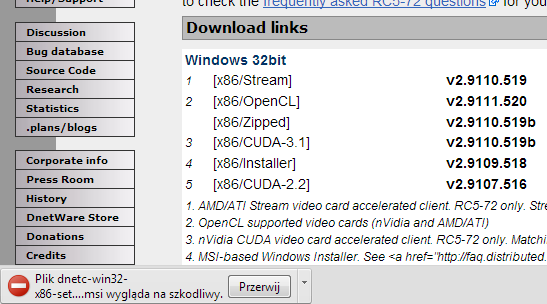
\includegraphics[width=0.5\textwidth]{distributedNet}
\caption{Pobranie aplikacji klienckiej powoduje wygenerowanie ostrze�enia dotycz�cego bezpiecze�stwa.}
\label{fig:distributedNet}
\end{figure}

Program \textit{distributed.net} trwa dalej mimo, �e RSA Laboratory wycofa�o si� ju� z fundowania nagr�d za �amanie kolejnych coraz to d�u�szych kluczy. Osoba chc�ca do��czy� do ochotnik�w nie ma jednak bardzo �atwego zadania i do��czanie do programu nie nale�y do przyjemnych. Nale�y wej�� na stron� \textit{distributed.net} i wybra� odpowiedni dla swojego systemu operacyjnego program kliencki. Wyb�r jest spory i mo�e przysporzy� problem�w mniej obeznanym w komputerach osobom, gdy� wyr�nione s� nie tylko nazwy system�w, ale i architektury (np. Windows x86/CUDA-2.2, x86/CUDA-3.1). Po zdecydowaniu si� ju� na kt�ry� z program�w i po zako�czeniu pobierania, mo�e  dosta� gro�nie wygl�daj�cy komunikat w kt�rym jego system operacyjny ostrze�e go �e program jest potencjalnie szkodliwy dla komputera, jak przedstawiono na rycinie \ref{fig:distributedNet} na stronie ~\pageref{fig:distributedNet}.

Ufaj�c dostawcy, po zdecydowaniu si� na zainstalowanie programu, otwiera si� bardzo ma�o przyjazny interfejs konsolowy, kt�ry wida� na rycinie \ref{fig:distributedNetConsole} na stronie ~\pageref{fig:distributedNetConsole}.

\begin{figure}[h]
\centering
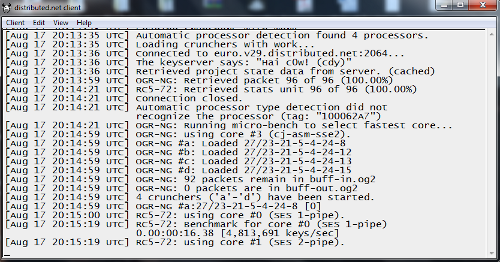
\includegraphics[width=0.5\textwidth]{distributedNetConsole}
\caption{Ma�o przyjazny interfejs konsolowy programu \textit{distributed.net}}
\label{fig:distributedNetConsole}
\end{figure}

Nasz wniosek jest taki, �e przestarza�e i nieatrakcyjne systemy do Volunteer Computing nie maj� racji bytu w dzisiejszym �wiecie i pr�dzej czy p�niej wygin� na rzecz rozwi�za� bardziej przyjaznych u�ytkownikowi.

\subsection{Berkeley Open Infrastructure for Network Computing}
\label{sec:BOINC}
Do stworzenia platformy BOINC (Berkeley Open Infrastructure for Network Computing), obecnie najbardziej znacz�cego open-source'owego middleware'u do oblicze� typu volunteer i grid computing, przyczyni� si� projekt SETI@home.

SETI@home to program rozpocz�ty w maju 1999 roku na uniwersytecie Berkeley, maj�cy na celu analiz� kosmicznego szumu radiowego i odnalezienie w nim sygna��w pochodz�cych od pozaziemskich cywilizacji. Przed migracj� do BOINC, projekt obs�ugiwa� system posiadaj�cy wiele luk bezpiecze�stwa. Kwestie, na kt�re na pocz�tku nie by�o nacisku, czyli wiarygodno�� zwracanych przez 'wolontariuszy' wynik�w, wraz z rozwojem projektu zacz�y odgrywa� coraz wi�ksze znaczenie, gdy� zauwa�ono, �e niekt�re rozwi�zanie by�y w ca�o�ci fa�szowane. 

Obecnie platforma BOINC umo�liwia weryfikacj� wynik�w. Opiera si� ona przede wszystkim na wysy�aniu tych samych zada� do wielu klient�w i por�wnywaniu wynik�w. W programie jest obecnie ponad 40 projekt�w. Instaluj�c klienta na swojej maszynie mo�na bra� udzia� w wybranych przez siebie projektach. 

Serwer BOINC mo�e by� uruchomiony na jednej lub wielu maszynach z systemem operacyjnym Linux, a oparty jest na technologiach Apache, PHP i MySQL.

Struktura klienta sk�ada si� z 

\begin{itemize}
\item programu \textit{boinc}, kt�ry zajmuje si� komunikacj� z serwerem oraz zarz�dzaniem aplikacjami naukowymi, kt�re wykonuj� ju� konkretne obliczenia
\item jednej lub wielu aplikacji naukowych. Aplikacja naukowa zwi�zana jest z konkretnym projektem, w kt�rym klient bierze udzia� i zajmuje si� obliczeniami dla dostarczonych jej cz�ci oblicze�. Uaktualnianiem aplikacji zajmuje si� \textit{boinc}
\item programu \textit{boincmgr} - GUI, kt�re komunikuje si� z \textit{boinc} przy u�yciu zdalnego wywo�ania procedur. GUI napisane jest w cross-platformowym toolkicie \textit{WxWidgets}. Poprzez GUI u�ytkownik mo�e wybra� nowe aplikacje naukowe, monitorowa� post�p prowadzonych przez siebie oblicze� oraz przegl�da� logi systemu BOINC
\item BOINC'owego wygaszacza ekranu. Jest to framework dzi�ki kt�remu aplikacje naukowe mog� wy�wietla� w atrakcyjny graficznie spos�b np. animacje czy te� wykresy wyja�niaj�ce prowadzone obliczenia
\end{itemize}

Obecnie prawie trzy miliony ludzi udost�pnia zasoby swoich osobistych komputer�w do oblicze� zwi�zanych tyko z projektem \textit{SETI@home}. Opiekunom projektu BOINC zale�y na rozwoju kultury udost�pniania swoich zasob�w na rzecz naukowych oblicze�. Interfejs systemu jest przyjazny, a sam system �atwy w instalacji.

\subsection{Urz�dzenia mobilne w rozproszonych obliczeniach naukowych}
\label{sec:mobilne}
Przez dziesi�ciolecia miliony ludzi udost�pnia�y zasoby swoich maszyn, aby wspom�c nauk�. Jednak komputery typu PC s� coraz mniej popularne, a ich sprzeda� spada o prawie 8 procent rocznie. Prognozy jasno wskazuj� na to, �e ten trend si� utrzyma. Z drugiej strony, bardzo dynamicznie rozwija si� rynek urz�dze� mobilnych, w tym smartphon�w. Wed�ug serwisu Bloomberg, do ko�ca roku 2013, na rynek zostanie dostarczonych 919 milion�w nowych urz�dze�, co jest 27 procentowym wzrostem w stosunku do roku 2012. %TODO  ANia latexowe odniesienie do pozycji BOINCAndroid z bibliografi

Do niedawna, telefony tego typu nie mia�y wystarczaj�cych zasob�w, by prowadzi� naukowe obliczenia. Obecnie maj� nawet cztery rdzenie i mog� wykonywa� p�tora miliarda operacji numerycznych na sekund�, co odpowiada oko�o jednej pi�tej tego co potrafi� wsp�czesne komputery osobiste. David Anderson, naukowiec z Berkeley, kt�ry wsp�tworzy mobiln� aplikacj�, kt�ra jest furtk� do naukowych oblicze� na smartphonach, twierdzi, �e jako, �e hardware mobilnych urz�dze� jest obecnie najbardziej rozwijan� ga��zi� urz�dze� elektronicznych, ju� wkr�tce, moc obliczeniowa tych urz�dze� mo�e wyr�wna� obecne osi�gi komputer�w osobistych. Mi�dzy innymi z tego powodu warto zacz�� uwzgl�dnia� urz�dzenia mobilne w roli potencjalnego wykonawcy intensywnych oblicze�.

Ciekawym konceptem jest obliczeniowa sie� stworzona z ogromnej liczby urz�dze�, kt�ra mog�aby rywalizowa� z takimi dostawcami us�ug jak Amazon Web Services. W tym momencie warto�� rynku komercyjnych oblicze� w chmurze osi�ga 131 miliard�w dolar�w. Sie� stworzona z telefon�w mo�e by� tanim odpowiednikiem i umo�liwi� na przyk�ad firmie farmaceutycznej p�aci� po kilkadziesi�t cent�w miesi�cznie za udost�pnienie swojego urz�dzenia np. przez noc do potrzebnych jej oblicze�. Wizj� t� roztacza Bernie Meyerson, wiceprezydent innowacji w firmie IBM. %TODO Ania - te wsyztskie dane sa z tego artyku�u z Bloomberga BOINCAndorid w bibliografi. Oznacz to prosz� tak �eby byKo dobrze

W sierpniu 2013 w g��wnym sklepie z aplikacjami na system Android - Google Play, pojawi�a si� oficjalna aplikacja stworzona przez zesp� BOINC z Berkeley. Aplikacja umo�liwia posiadaczowi smartphona w bardzo przyjazny spos�b na do��czenie do oblicze�. 
Rozwa�anie u�ycia urz�dze� mobilnych do oblicze� wywo�uje pytanie o zu�ycie baterii. Aplikacja zaprojektowana jest tak, by da� u�ytkownikowi pe�n� kontrol� nad tym jakie warunki musz� zaj��, aby prowadzone by�y obliczenia (implikuj�ce szybsze zu�ycie baterii). Warunkami tymi mo�e by� np. pod��czenie do �r�d�a zasilania oraz poziom zu�ycia baterii powy�ej zadanego progu.

\begin{figure}[h]
\centering
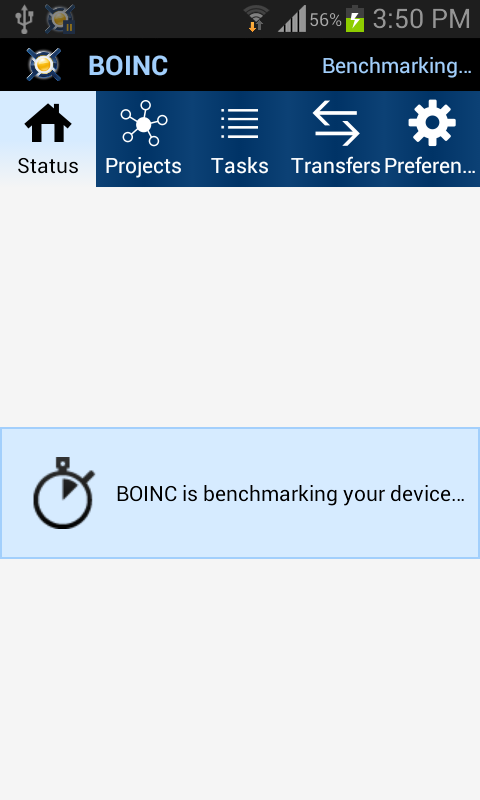
\includegraphics[height=200px]{boinc-app-benchmark}
\caption{Proces benchmarkowania urz�dzenia, po pierwszym uruchomieniu aplikacji BOINC na system Android}
\label{fig:boinc-app-benchmark}
\end{figure}

\begin{figure}[h]
\centering
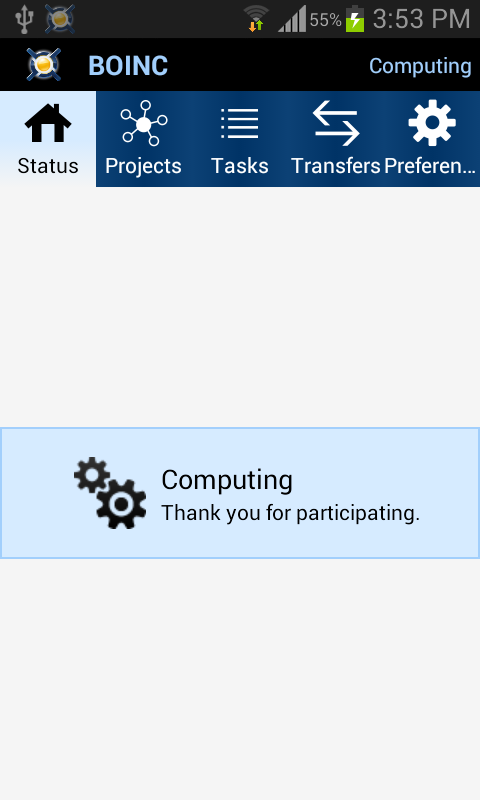
\includegraphics[height=200px]{boinc-app}
\caption{Aplikacja BOINC w trakcie oblicze� dokonywanych na platformie z systemem Android}
\label{fig:boinc-app}
\end{figure}

\subsection{Folding@home}
\label{sec:folfingathome}
Projekt wywodz�cy si� z Ameryka�skiego Uniwersytetu Stanford by� pierwszym, kt�ry zauwa�y�, �e potencja� Volunteer Computing nie zamyka si� tylko na komputery osobiste i wykorzystanie jednostek CPU, ale tak�e coraz bardziej rozwijanych jednostek GPU, procesor�w na PlayStation 3. Jako pierwszy du�y projekt wykorzysta� te� model Message Passing Interface. Pojedynczy klienci dostaj� z serwera cz�� symulacji i po jej wykonaniu odsy�aj� j� z powrotem do serwera, w kt�rym cz�ci s� ��czone i stwarzaj� ca�o�ciow� symulacj�. Co ciekawe, ochotnicy bior�cy udzia� w symulacjach, mog� �ledzi� sw�j wk�ad w projekt Folding@home poprzez stron� internetow�. Obserwujemy, �e techniki rywalizacyjne zacz�y by� coraz szerzej wprowadzane do projekt�w Volunteer Computing w celu utrzymania zainteresowania ochotnik�w w braniu udzia�u w projekcie.

\begin{figure}[h]
\centering
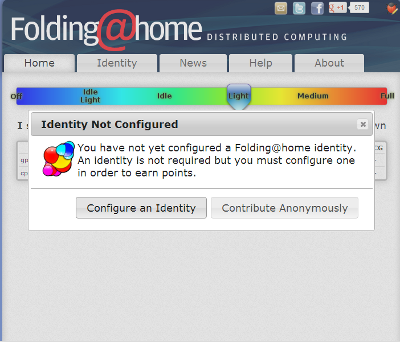
\includegraphics[width=0.5\textwidth]{foldingStart}
\caption{Przyjazny u�ytkownikowi ekran powitalny interfejsu aplikacji \textit{Folding@home}}
\label{fig:foldingStart}
\end{figure}

\begin{figure}[h]
\centering
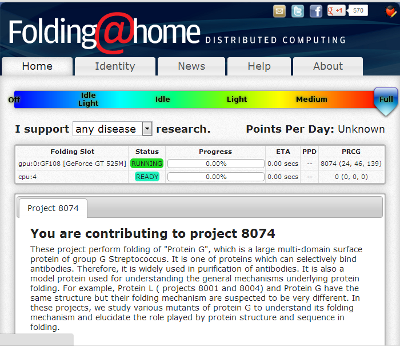
\includegraphics[width=0.5\textwidth]{foldingMonitor}
\caption{Monitorowanie post�pu oblicze� poprzez interfejs aplikacji\textit{Folding@home}}
\label{fig:foldingMonitor}
\end{figure}

Folding@home jest jednym z najwi�kszych system�w komputerowych na �wiecie. Jego szybko�� szacuje si� na oko�o 14 petaflops'�w na sekund�, wi�cej ni� wszystkich projekt�w, kt�re s� przetwarzane na wywodz�cej si� z Berkeley platformie BOINC. W 2007 zosta� wpisany do ksi�gi rekord�w Guinessa jako system rozproszonych oblicze� o najwi�kszej mocy obliczeniowej. Stan na Czerwiec 2013 wskazuje prawie p� miliona aktywnych CPU oraz prawie 25 tysi�cy aktywnych GPU.

Folding@home wprowadza elementy rywalizacyjne poprzez wprowadzenie systemu punktowego. Osoby udost�pniaj�ce swoje zasoby dostaj� punkty za ka�de wykonane zadanie, dodatkowe punkty mo�na zdobywa� za szybkie wykonanie pewnych zada�, kt�re s� szczeg�lnie wymagaj�ce obliczeniowo albo maj� wi�kszy priorytet ze wzgl�du na warto�� naukow�. Gromadzi� wi�cej punk�w mo�na dzi�ki w��czeniu do programu, pod jednym loginem, wielu swoich maszyn. Og�lnym za�o�eniem systemu punktowego jest motywowanie ochotnik�w do coraz wi�kszego zaanga�owania i w��czania znajomych do wsp�lnej zabawy ��czonej z rywalizacj�. Statystyki, zar�wno poszczeg�lnych dru�yn, jak i indywidualnych os�b s� widoczne na stronie g��wnej projektu.

Oprogramowanie Folding@Home jest przyjazne. �ci�gni�cie i instalacja nie powoduje �adnych niepokoj�cych ostrze�e� ze strony systemu operacyjnego. Interfejs kliencki jest interfejsem webowym, ��cz�cym si� z nadaj�c� na lokalnej maszynie aplikacj� klienck� wykonuj�c� obliczenia. Tw�rcy platformy staraj� si� u�atwi� rozprzestrzenianie si� informacji o mo�liwo�ci kontrybuowania do naukowego projektu daj�c mo�liwo�� udost�pniania informacji o programie poprzez portale spo�eczno�ciowe takie jak Facebook czy Twitter.


\begin{figure}[h]
\centering
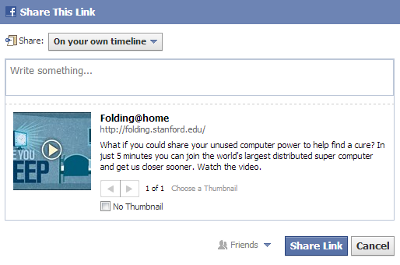
\includegraphics[width=0.4\textwidth]{foldingShare}
\caption{Zach�canie do udost�pniania informacji o programie \textit{Folding@home} w sieciach spo�eczno�ciowych}
\label{fig:foldingShare}
\end{figure}



\chapter{Proponowane rozwi�zanie}
\label{cha:rozwiazanie}

W rozdziale tym przedstawiono informacje dotycz�ce zastosowanego rozwi�zania. Opisane zosta�y przyj�te za�o�enia dotycz�ce modelu, matematyczny opis tego modelu oraz szczeg�y zastosowanego sposobu optymalizacji. Na ko�cu rozdzia�u przedstawiona zosta�a architektura rozwi�zania wraz z opisem powsta�ej aplikacji ko�cowej.

%---------------------------------------------------------------------------

\section{Model narciarza i �rodowiska}
\label{sec:model}

W zaproponowanym rozwi�zaniu zosta�y podj�te pewne decyzje odno�nie reprezentacji �rodowiska oraz narciarza.

Zosta�o przyj�te, �e stok traktowany jest jako p�aszczyzna, kt�ra jest nachylona do powierzchni ziemi pod k�tem pod okre�lonym przez sta�� $\alpha$. Za�o�enie co do p�askiej powierzchni stoku jest tylko ograniczeniem przyj�tym do test�w. Umo�liwia to �atwiejsz� analiz� wynik�w, niezaburzonych zmianami nachylenia terenu. Jednak stworzony program mo�e zosta� w prosty spos�b zmodyfikowany tak, aby zamodelowa� r�wnie� bardziej skomplikowan� powierzchni�.

Narciarz traktowany jest jako punkt materialny o masie m.
%---------------------------------------------------------------------------

\section{Opis matematyczny modelu}
\label{sec:matematycznyModel}

Oznaczenia:
\begin{itemize}
\item m - masa
\item g - przyspieszenie ziemskie
\item $\alpha$ - k�t nachylenia stoku
\end{itemize}

Si�a grawitacji dzia�aj�ca na obiekt o masie m:\\
\begin{equation}
Q = mg
\end{equation}

Si�a ta mo�e zosta� roz�o�ona na dwie sk�adowe wzgl�dem powierzchni stoku:
\begin{itemize}
\item r�wnoleg��, wynosz�c� $Q_a$,
\item prostopad�� $F_n$.
\end{itemize}
Narciarz poruszaj�cy si� w d� stoku jest modelowany jako punkt materialny poruszaj�cego si� po r�wni pochy�ej. Rozk�ad si� w takim przypadku rozrysowany jest na rysunku \ref{fig:inclinedPlane}.\\

\begin{figure}[h]
\centering
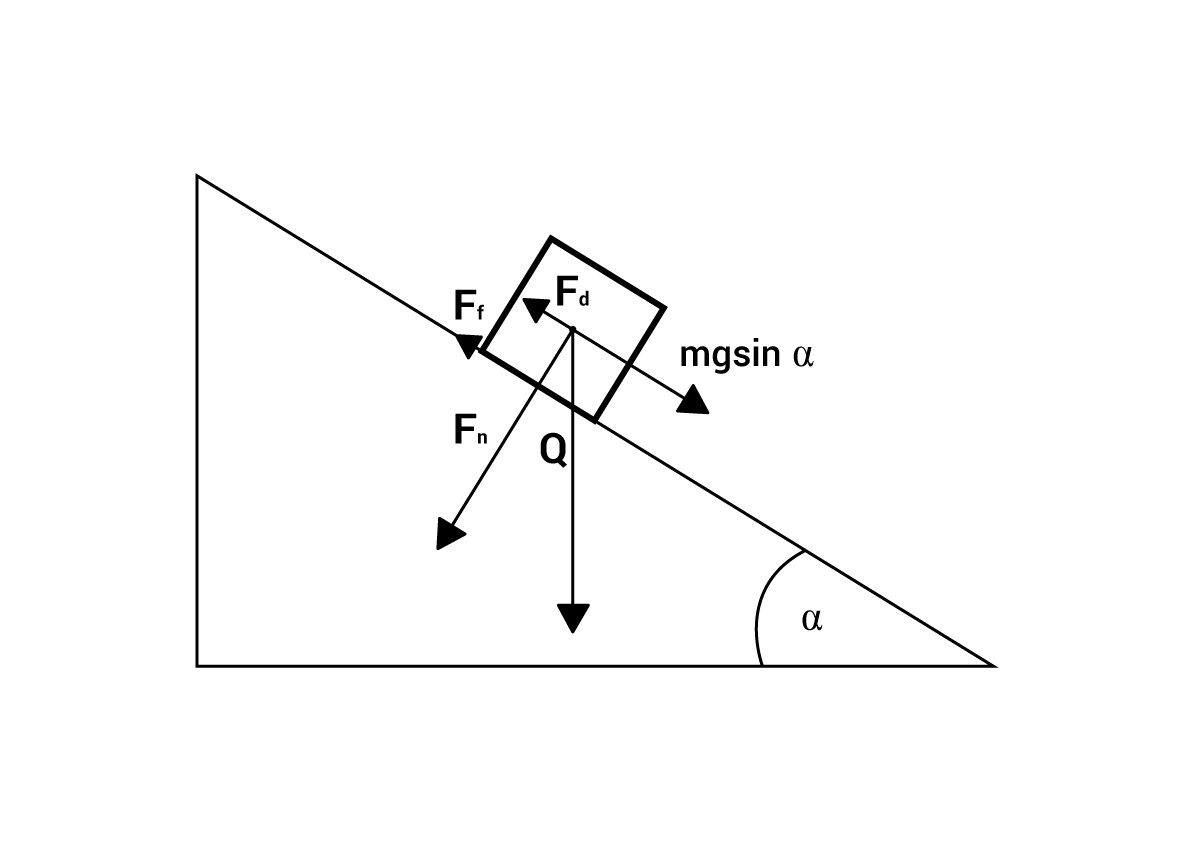
\includegraphics[scale=0.4]{model/inclinedPlane}
\caption{Rozk�ad si� dzia�aj�cych na narciarza przemieszczaj�cego si� na r�wni pochy�ej}
\label{fig:inclinedPlane}
\end{figure}

Sk�adowa si�y grawitacji r�wnoleg�a do powierzchni stoku jest r�wna:\\
\begin{equation}
\label{eq:Qa}
Q_a = mg\sin\alpha
\end{equation}

Si�a $Q_a$ jest si�� �ci�gaj�c� narciarza w d� stoku.

Sk�adowa si�y grawitacji prostopad�a do powierzchni stoku, czyli nacisk jaki narciarz wywiera swoj� mas� na powierzchni� stoku, jest r�wna:\\
\begin{equation}
\label{eq:Fn}
F_n = mg\cos\alpha
\end{equation}

Warto�� tej si�y wp�ywa na si�� tarcia dzia�aj�cej na narciarza:\\
\begin{equation}
\label{eq:Ff}
F_f = \mu F_n = \mu mg\cos\alpha
\end{equation}

Opr�cz si�y tarcia uwzgl�dniamy r�wnie� si�� oporu powietrza. Zale�y ona od pr�dko�ci poruszania si� obiektu. Pr�dko�� b�dziemy wyra�a� jako pierwsz� pochodn� po�o�enia, oznaczan� przez $ \dot{x} $:\\
\begin{equation}
\label{eq:Fd}
F_d = k\dot{x}^2
\end{equation}


\begin{equation}
k = \frac{1}{2} C \rho A
\end{equation}

gdzie:\\
$ C $ - wsp�czynnik oporu\\
$ \rho $ - g�sto�� powietrza\\
$ A $ - powierzchnia narciarza prostopad�a do kierunku ruchu

Wi�cej o sile oporu powietrza jest opisane w sekcji \ref{sec:oporPowietrza} na stronie \pageref{sec:oporPowietrza}.

%---------------------------------------------------------------------------

\section{Numeryczne rozwi�zanie problemu}
\label{sec:numeryczneRozwiazanie}

Z drugiej zasady dynamiki Newton'a wiemy, �e:

\begin{equation}
m\overrightarrow{a} = \sum\limits_i{\overrightarrow{F_i}}
\end{equation}

Rozpatruj�c wszystkie si�y dzia�aj�ce na narciarza r�wnoleg�e do powierzchni stoku, a wi�c powoduj�ce jego ruch w d�, otrzymujemy nast�puj�ce r�wnanie ruchu:

\begin{equation}
m\overrightarrow{a} = \overrightarrow{Q_a} + \overrightarrow{F_f} + \overrightarrow{F_d}
\end{equation}

A zatem, uwzgl�dniaj�c kierunek si� otrzymujemy:

\begin{equation}
ma = Q_a - F_f - F_d
\end{equation}

Wypadkowa si�a dzia�aj�ca na narciarza jest sum� si�: �ci�gaj�cej oraz opor�w (tarcia i oporu powietrza).

Korzystaj�c z wcze�niejszych r�wna� \ref{eq:Qa}, \ref{eq:Ff} i \ref{eq:Fd} opisuj�cych si�y $ Q_a $, $F_f$ oraz $ F_d $ otrzymujemy:

\begin{equation}
ma = mg\sin\alpha - \mu mg\cos\alpha - k\dot{x}^2
\end{equation}

Wyra�my teraz przyspieszenie jako drug� pochodn� przemieszczenia:

\begin{equation}
a = \ddot{x} 
\end{equation}

Podstawiaj�c do r�wnania:

\begin{equation}
m\ddot{x}=mg\sin\alpha-\mu mg\cos\alpha - k\dot{x}^2
\end{equation}

Zatem po podzieleniu przez m:

\begin{equation}
\label{eq:rownRuchu}
\ddot{x}=g\sin\alpha-\mu g\cos\alpha - \frac{k}{m}\dot{x}^2
\end{equation}

Jest to r�wnanie r�niczkowe zwyczajne drugiego rz�du. Aby rozwi�za� to r�wnanie numerycznie, przedstawimy to r�wnanie jako uk�ad r�wna� r�niczkowych zwyczajnych rz�du pierwszego. W tym celu wprowadzamy now� zmienn� v (odpowiadaj�c� pr�dko�ci) b�d�c� pierwsz� pochodn� przemieszczenia, a drug� pochodn� zast�pujemy pierwsz� pochodn� pr�dko�ci:

\begin{equation}
\left\{ \begin{array}{ll}
v = \dot{x}	\\
\ddot{x} = \dot{v}
\end{array} \right. 
\end{equation}

Zatem wykorzystuj�c powy�sze r�wnania otrzymujemy nast�puj�cy uk�ad r�wna�:\\
\begin{equation}
\label{eq:ur2d}
\left\{ \begin{array}{ll}
\dot{v} = gsin\alpha-\mu gcos\alpha-\frac{k}{m}v^{2} \\
v = \dot{x}
\end{array} \right. 
\end{equation}


W wielu j�zykach programowania dost�pne s� funkcje biblioteczne, kt�re potrafi� znale�� rozwi�zanie uk�adu r�wna� r�niczkowych zwyczajnych pierwszego rz�du, takich jak nasz uk�ad \ref{eq:ur2d}. W celu jego rozwi�zania zosta�a wykorzystana funkcja dopri (ang. \textit{Numerical integration of ODE using Dormand-Prince RK method}) z biblioteki Numeric Javascript.

\subsection{Rozwi�zanie na p�aszczy�nie stoku}
\label{subsec:3d}
Powy�szy uk�ad r�wna� (\ref{eq:ur2d}) opisuje poruszanie si� punktu materialnego po r�wni pochy�ej. Jednak w przypadku narciarza przemieszczaj�cego si� po stoku musimy uwzgl�dni� r�wnie� mo�liwo�� poruszania si� w poprzek stoku, a nie tylko w d�.\\
Za��my, �e narciarz porusza si� po torze b�d�cym �aman�. W dalszej cz�ci pracy zostanie pokazane, �e takie ograniczenie mo�e by� dobrym sposobem na przybli�enie rzeczywistego toru jazdy, kt�re jednocze�nie znacznie u�atwia sterowanie ruchem narciarza. \\

Rozpatrzmy teraz jak b�dzie wygl�da� uk�ad si� dzia�aj�cych na narciarza (\ref{fig:stok3d}):\\

\begin{figure}[H]
\centering
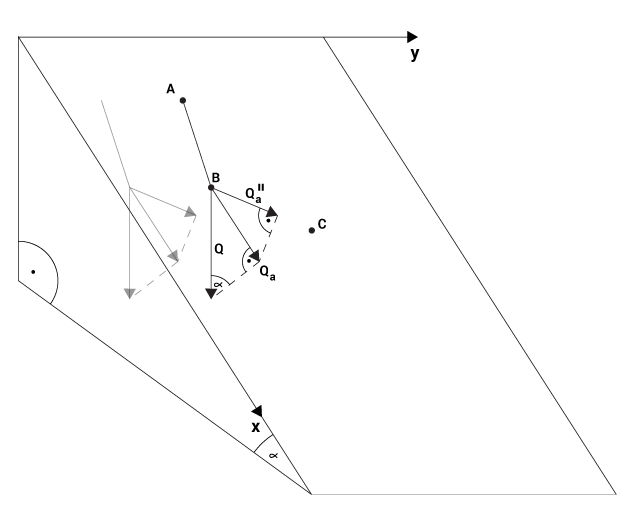
\includegraphics[scale=1]{model/stok3d}
\caption{Rozk�ad wybranych si� dzia�aj�cych na narciarza przemieszczaj�cego si� na p�aszczy�nie stoku}
\label{fig:stok3d}
\end{figure}

Na p�aszczy�nie stoku zosta�y oznaczone trzy punkty - $A$, $B$ i $C$, przez kt�re kolejno przeje�d�a narciarz. Zak�adaj�c, �e narciarz znajduje si� w punkcie $B$, oznaczona zosta�a si�a grawitacji $Q$, dzia�aj�ca na niego i skierowana pionowo (w stosunku do powierzchni ziemi). Sk�adowa tej si�y - $Q_a$, jest rzutem na powierzchni� stoku i jest r�wna (jak w przypadku r�wnania \ref{eq:Qa}):

\begin{equation}
Q_a = mg\sin\alpha
\end{equation}

$\alpha$ jest k�tem nachylenia p�aszczyzny stoku. Po zrzutowaniu si�y $Q_a$ na odcinek $BC$ otrzymujemy si�� $Q_a^\|$ - jej kierunek jest zgodny z kierunkiem poruszania si� narciarza. Pozosta�e sk�adowe si� $Q$ oraz $Q_a$ s� r�wnowa�one przez si�� reakcji pod�o�a wywieran� na narciarza.

\begin{figure}[H]
\centering
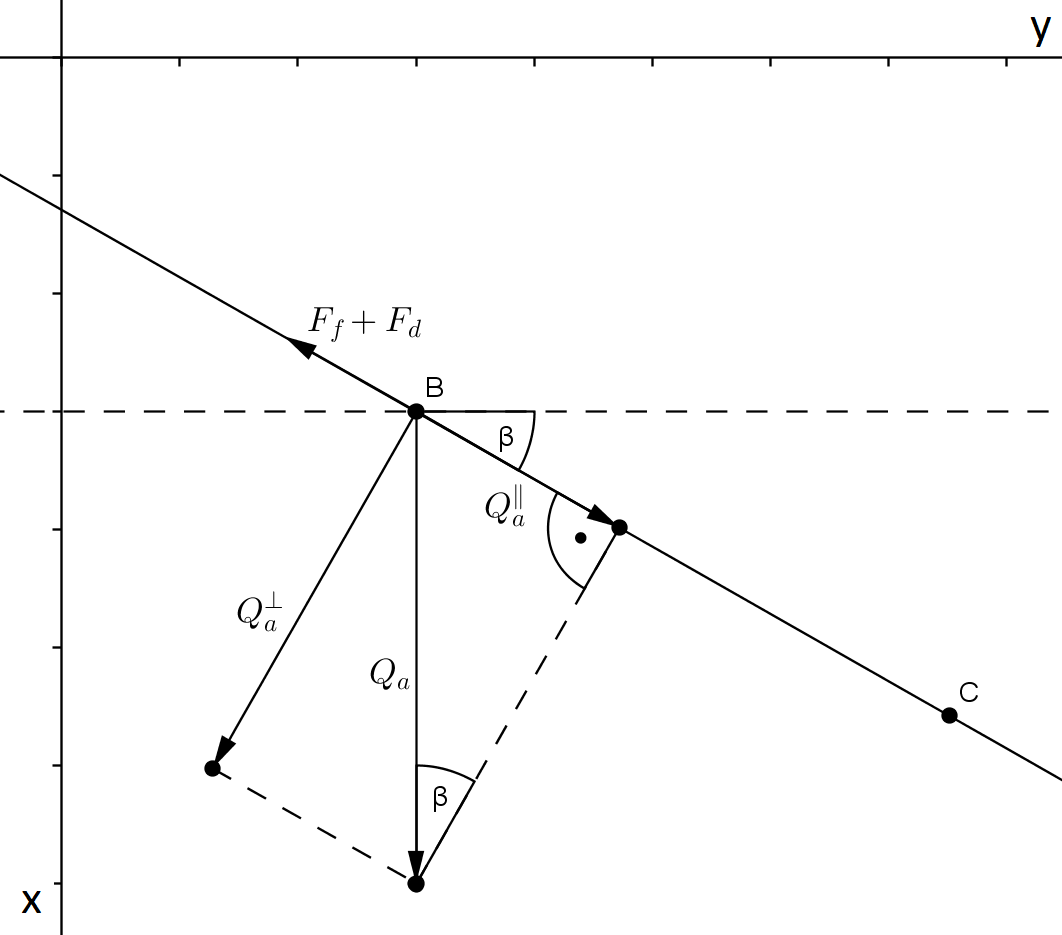
\includegraphics[scale=0.5]{model/stok2d}
\caption{Rozk�ad wybranych si� dzia�aj�cych na narciarza przemieszczaj�cego si� na p�aszczy�nie stoku}
\label{fig:stok2d}
\end{figure}

Na rysunku \ref{fig:stok2d} przedstawiona zosta�a p�aszczyzna stoku z punktami $B$ i $C$ oraz si�ami $Q_a$ oraz jej sk�adowymi $Q_a^\|$ oraz $Q_a^\bot$. K�t $\beta$ jest k�tem pomi�dzy wektorem przemieszczenia a poziom� lini� na p�aszczy�nie stoku. Warto�� si�y �ci�gaj�cej wynosi w tym przypadku:

\begin{equation}
Q_a^\| = mg\sin\alpha \sin\beta
\end{equation}

Zaznaczone zosta�a r�wnie� si�a stanowi�ca sum� si� opor�w $F_f + F_d$. Zatem nasze r�wnanie ruchu \ref{eq:rownRuchu} b�dzie wygl�da�o nast�puj�co:

\begin{equation}
\ddot{x} = g\sin\alpha \sin\beta - \frac{F_f + F_d}{m}
\end{equation}

Wykorzystuj�c wzory na si�y opor�w (\ref{eq:Ff} oraz \ref{eq:Fd}) otrzymamy:

\begin{equation}
\ddot{x} = g\sin\alpha \sin\beta - \frac{\mu F_n  + k\dot{x}^2}{m}
\end{equation}

gdzie $F_n$ to si�a nacisku narciarza, kt�ra pozostaje taka sama jak w przypadku r�wni pochy�ej (\ref{eq:Fn}):

\begin{equation}
F_n = mg\cos\alpha
\end{equation}

Zatem:

\begin{equation}
\ddot{x} = g\sin\alpha \sin\beta - (\mu g\cos\alpha  + \frac{k}{m}\dot{x}^2)
\end{equation}

W naszym rozwi�zaniu zastosowany zosta� zaznaczony na rysunku uk�ad wsp�rz�dnych XY. Powy�sze r�wnanie zapiszmy teraz uwzgl�dniaj�c przemieszczanie si� narciarza w oznaczonych kierunkach - wzd�u� i wszerz stoku. Otrzymamy wtedy nast�puj�ce r�wnania:

\begin{equation}
\label{eq:ur2rzedu}
\left\{ \begin{array}{ll}
\ddot{x_x} = (g\sin\alpha\sin\beta - (\mu g\cos\alpha + \frac{k}{m}\dot{x}^2))\sin\beta\\
\ddot{x_y} = (g\sin\alpha\sin\beta - (\mu g\cos\alpha + \frac{k}{m}\dot{x}^2))\cos\beta
\end{array} \right.
\end{equation}

Po wprowadzeniu jak poprzednio dodatkowych zmiennych, aby zredukowa� r�wnania do r�wna� r�niczkowych zwyczajnych pierwszego rz�du, wprowadzamy dodatkowe zmienne, w tym wypadku pr�dko�ci $v_x$ i $v_y$ oraz pami�tamy o zale�no�ci mi�dzy nimi a pochodn� przemieszczenia:

\begin{equation}
\left\{ \begin{array}{ll}
v_x = \dot{x_x}\\
v_y = \dot{x_y}\\
\dot{x} = \sqrt{v_x^2 +v_y^2}
\end{array} \right.
\end{equation}

Dodatkowo mo�na zauwa�y�, �e je�li $v_x$ stanowi pierwsz� pochodn� $ x_x $ to prawdziwe s� tak�e poni�sze r�wnania:
 
\begin{equation}
\left\{ \begin{array}{ll}
\dot{v_x} = \ddot{x_x}\\
\dot{v_y} = \ddot{x_y}\\
\end{array} \right.
\end{equation}

Wprowadzaj�c te informacje do uk�adu r�wna� \ref{eq:ur2rzedu}, otrzymujemy:

\begin{equation}
\left\{ \begin{array}{ll}
v_x = \dot{x_x}\\
v_y = \dot{x_y}\\
\dot{v_x} = (g\sin\alpha\sin\beta - (\mu g\cos\alpha + \frac{k}{m}\dot{x}^2))\sin\beta\\
\dot{v_y} = (g\sin\alpha\sin\beta - (\mu g\cos\alpha + \frac{k}{m}\dot{x}^2))\cos\beta
\end{array} \right. 
\end{equation}\\

Taki uk�ad r�wna� r�niczkowych mo�na rozwi�za� wspomnian� wcze�niej funkcj� \textit{dopri}. 

%---------------------------------------------------------------------------

\section{Optymalizacja toru przejazdu}
\label{sec:optymalizacja}
Aby znale�� rozwi�zanie problemu optymalizacji, nale�y przyj�� jaki� spos�b reprezentacji ka�dego z rozwi�za�. W rzeczywisto�ci tor przejazdu narciarza to �lad, kt�ry pozostawiaj� narty na �niegu w trakcie przemieszczania si� po stoku. Jak opisano w podrozdziale \ref{subsec:3d}, w celu uproszczenia sposobu przemieszczania si� narciarza, zdecydowano, �e b�dzie si� on porusza� po �amanej. Zatem do reprezentacji rozwi�zania mo�na przyj�� zbi�r punkt�w, przez kt�re kolejno przeje�d�a narciarz, poruszaj�c si� mi�dzy tymi punktami wy��cznie po linii prostej.

\begin{figure}[h]
\centering
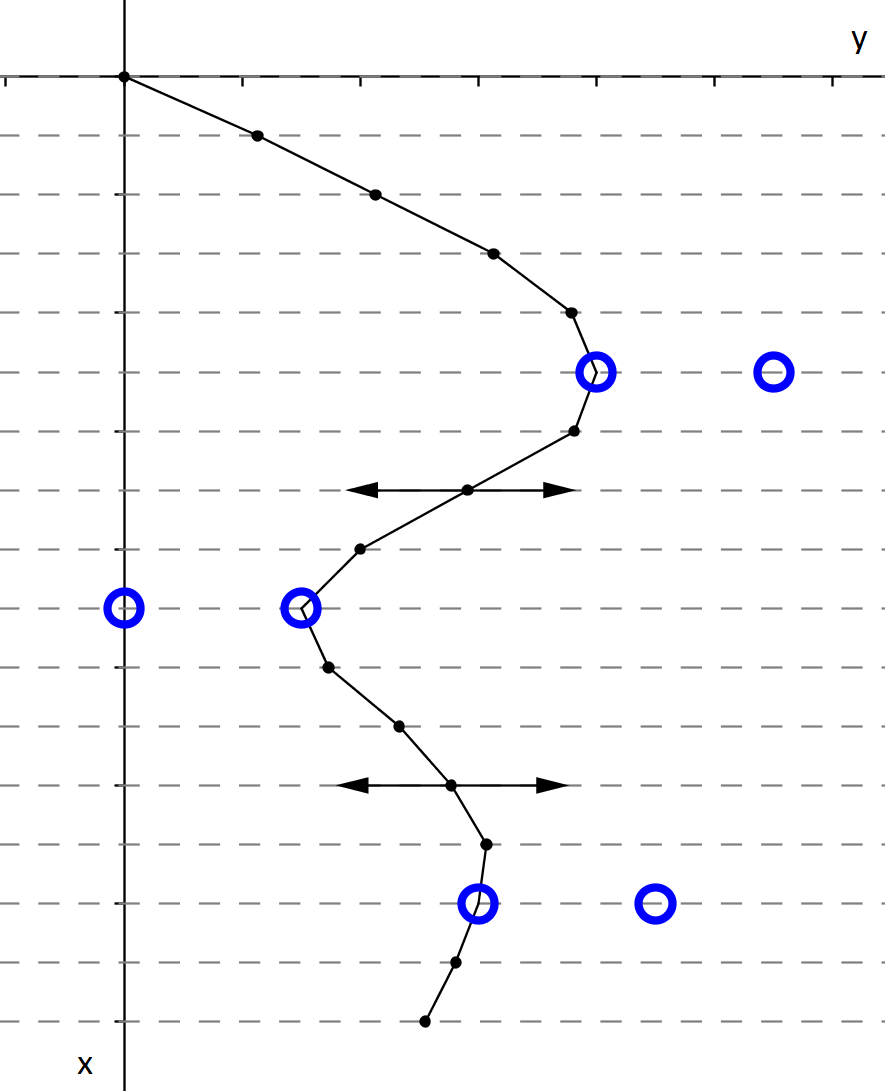
\includegraphics[scale=0.5]{model/lamana}
\caption{Spos�b reprezentacji rozwi�za� problemu}
\label{fig:lamana}
\end{figure}

W zaproponowanym rozwi�zaniu narzucamy z g�ry, co ile metr�w w pionie stoku ma znajdowa� si� punkt, przez kt�ry b�dzie musia� przejecha� narciarz. Mo�na wyobrazi� to sobie jako zbi�r poziomych linii, z kt�rej ka�da wyznacza mo�liwe po�o�enie pojedynczego punktu. Na rysunku \ref{fig:lamana} zosta�y przedstawione te linie oraz bramki (kolor niebieski). Strza�ki pokazuj� jak mo�na przesuwa� ka�dy z tych punkt�w w celu zmiany trasy przejazdu i otrzymania nowego rozwi�zania. Zosta�o narzucone, �e narciarz musi przejecha� jak najbli�ej ka�dej wewn�trznej cz�ci bramki, co oznacza do�o�enie punkt�w w tym miejscu. Ogranicza to znacznie liczb� rozwi�za�, kt�re nale�y sprawdzi� i dzi�ki temu przyspiesza dzia�anie algorytmu. Takie za�o�enie bazuje r�wnie� na do�wiadczeniu narciarzy z jazdy po slalomach, gdy� w wi�kszo�ci przypadk�w przeje�d�anie tu� przy bramkach jest najkorzystniejsze. Zdarza si� oczywi�cie, �e np. dla tzw. bramek otwartych opisanych w rozdziale \ref{sec:alpineSkiing} cz�sto lepiej wybra� troch� inn� tras�. W tych przypadkach konieczne jest zrezygnowanie z takiego ograniczenia, jednak nale�y liczy� si� z tym, �e czas poszukiwania najlepszego rozwi�zania wyd�u�y si�, zw�aszcza je�li takich miejsc jest wi�cej.

Zatem pozostaje okre�li�, w jaki spos�b mo�emy stwierdzi�, �e dane rozwi�zanie jest najlepsze. W tym przypadku chcemy, aby narciarz w jak najkr�tszym czasie dotar� do mety prawid�owo przeje�d�aj�c przez wszystkie bramki. Maj�c dane rozwi�zanie w postaci punkt�w wyznaczaj�cych �aman�, obliczamy ile czasu zajmie narciarzowi przejechanie po tej trasie. Im mniejsza warto�� tym rozwi�zanie jest lepsze. Zatem funkcja celu dla tego problemu maj�c na wej�ciu ci�g punkt�w wyznaczaj�cych tras� przejazdu, zwraca czas potrzebny na jej pokonanie.

\subsection{Algorytm ewolucyjny}
\label{sec:ewolucyjnyRozw}
Opisana w poprzednim podrozdziale reprezentacja rozwi�zania to w zastosowanym algorytmie ewolucyjnym pojedynczy osobnik, a punkty sk�adaj�ce si� na to rozwi�zanie, a �ci�lej, ich po�o�enie w pozycji poziomej, okre�laj� genotyp ka�dego osobnika. Poniewa� korzystamy ze strategii ewolucyjnych, nie wprowadzamy tu kodowania binarnego, pozycja ka�dego punktu jest zapami�tywana jako warto�� rzeczywista.

Dodatkowo do genotypu wchodzi tak�e zestaw parametr�w $\sigma$, kt�re w strategiach ewolucyjnych u�ywane s� podczas mutacji, tak jak opisano to w rozdziale \ref{sec:ewolucyjny} w cz�ci ``Typy algorytm�w ewolucyjnych'' w opisie strategii ewolucyjnych. Ka�demu punktowi przypisana jest osobna warto�� $\sigma$ - reprezentuj�ca odchylenie standardowe warto�ci $y$ tego punktu.

Zastosowany algorytm wykorzystuje strategi� ($\mu$ + $\lambda$) opisan� w rozdziale \ref{sec:ewolucyjny}. Jako pocz�tkow� populacj� wybieramy losowe osobniki - warto�ci $y$ punkt�w s� ograniczone jedynie przez warto�ci $y$ po�o�enia dw�ch najbli�szych bramek. Jest to kierowane konieczno�ci� zadbania o szybsze znalezienie rozwi�zania - zbyt du�e odleg�o�ci mo�na z g�ry odrzuci� opieraj�c si� na do�wiadczeniach z rzeczywistej jazdy narciarza po slalomie. Wielko�� populacji bazowej $\mu$ jest jednym z parametr�w programu, warto�� ta wynosi w testach 30 - 60. Warto�� parametru $\lambda$ tak�e jest parametrem, w testach u�yto wielko�ci 100 - 200. Warto�ci te por�wnywalne s� z sugerowanymi w literaturze. \cite{arabas}

Szkielet algorytmu zgodny jest z zastosowan� strategi� - po wylosowaniu z istniej�cej populacji populacji tymczasowej o wielko�ci $\lambda$, dokonuje si� na jej osobnikach operacji genetycznych, najpierw krzy�owania, a nast�pnie mutacji na osobnikach otrzymanych z krzy�owania. Kolejnym krokiem jest ocenienie nowych osobnik�w i wybranie spo�r�d nich oraz populacji pocz�tkowej osobnik�w o najlepszym przystosowaniu i to one stanowi� now� populacj� bazow�.

\subsubsection{Krzy�owanie}
Aby dokona� krzy�owania potrzebne s� pary rodzic�w dla ka�dego nowego osobnika. Aby utrzyma� wielko�� populacji tymczasowej, losujemy (ze zwracaniem) $\lambda$ par spo�r�d populacji tymczasowej. Krzy�owanie rodzic�w sprowadza si� do obliczenia �redniej warto�ci $y$ po�o�enia odpowiadaj�cych sobie punkt�w oraz parametr�w $\sigma$.

\subsubsection{Mutacja}
Po krzy�owaniu mamy znowu w populacji tymczasowej $\lambda$ osobnik�w. Mutacja osobnik�w przeprowadzana jest zgodnie ze strategi� - wykorzystywane s� warto�ci odchyle� standardowych odpowiadaj�cych kolejnym punktom. Jedynie punkty, kt�re s� przy bramkach nie podlegaj� mutacji. Wynika to z wcze�niejszego za�o�enia, �e i tak te punkty nale�� do rozwi�zania najlepszego.

\subsubsection{Warunek zako�czenia}
Wyb�r warunku zako�czenia algorytmu zawsze sprawia wiele problem�w. Nie jest �atwo zdecydowa� na jakiej podstawie zatrzymywa� jego dzia�anie. Cz�sto korzysta si� z informacji o rozrzucie przystosowania w populacji - obliczamy go na podstawie r�nicy pomi�dzy najlepszym i najgorszym osobnikiem. Je�li rozrzut ten jest niewielki mo�e oznacza� stagnacj� algorytmu. Niekoniecznie �wiadczy to o znalezieniu dobrego rozwi�zania, ale w po��czeniu z dodatkowymi mechanizmami mo�e by� skuteczn� metod� podj�cia decyzji o zako�czeniu optymalizacji.

W rozwi�zaniu brany jest zatem r�wnie� pod uwag� taki wska�nik jak poprawa najlepszego obecnego rozwi�zania. Je�li przez okre�lon� liczb� iteracji, najcz�ciej kilka lub kilkana�cie, najlepsze rozwi�zanie nie poprawia si� w og�le, a populacja jest bardzo ma�o zr�nicowana to jest to znak, �e znalezione rozwi�zanie powinno by� wystarczaj�co bliskie najlepszego. Oczywi�cie steruj�c liczb� iteracji, przez kt�re sprawdzamy zmiany, oraz wielko�ci� rozrzutu populacji mo�emy znajdowa� lepsze lub gorsze rozwi�zania kosztem wyd�u�enia lub skr�cenia czasu oblicze�.

\subsection{Hill climbing}
Problem optymalizacji trasy narciarza mo�na rozwi�zywa� stosuj�c algorytm ewolucyjny, jednak problemem mo�e by� d�ugi czas wykonywania si� programu. S�aba poprawa wynik�w mo�e wyst�powa� zw�aszcza w ko�cowej fazie dzia�ania. Widoczne s� wtedy niepotrzebne pr�by przeszukiwania zbyt odleg�ych rozwi�za�, a jednak wci�� znalezione rozwi�zanie nie jest jeszcze tak dobre, jak mo�na by tego oczekiwa�. Wiedz�c, �e rozwi�zanie jest ju� dosy� bliskie najlepszemu mo�na z du�ym prawdopodobie�stwem za�o�y�, �e wystarczy znale�� rozwi�zanie lokalnie optymalne, aby by�o ono satysfakcjonuj�ce. Oczywi�cie nie mamy pewno�ci, �e b�dzie to rozwi�zanie globalnie optymalne, ale najcz�ciej takiej pewno�ci mie� nie mo�emy. Problemem mo�e wci�� by� jednak decyzja kiedy nale�y przej�� na algorytm lokalnej optymalizacji.

Zastosowanie algorytmu lokalnej optymalizacji powinno pom�c w ko�cowej fazie poszukiwa�. Z tego powodu u�yty zosta� algorytm Hill climbing opisany w rozdziale \ref{sec:hill}. W ka�dym kroku algorytmu sprawdzane jest czy zmiana pojedynczej zmiennej - w tym wypadku poziomej pozycji punktu przejazdu, daje popraw� wyniku. Je�li zmiany te nie przynosz� znacz�cych rezultat�w, s� mniejsze ni� narzucony parametr $\epsilon$, algorytm zatrzymuje swoje dzia�anie. Warto�� $\epsilon$ wynosi przewa�nie w testach 0.00001. W przypadku parametr�w typowych dla tego algorytmu postanowiono wybra� warto�ci: dla przyspieszenia standardowa - 1.2, natomiast dla kroku, mniejsz� ni� zwykle, bo wynosz�c� 0.5 (odpowiada to wielko�ci 0.5 metra). Zmiana ta wynika z za�o�enia, �e aby znale�� rozwi�zanie jak najlepsze, nie trzeba zmienia� warto�ci $y$ �adnego z punkt�w o wi�cej ni� wybrane 0.5 m.

%---------------------------------------------------------------------------

\section{Modelowanie karania}
\label{sec:karanie}

W celu jak najdok�adniejszego zamodelowania zmian pr�dko�ci podczas poruszania si� po �amanej, testowany by� szereg modeli. Konieczno�� wprowadzenia takich mechanizm�w staje si� oczywista, gdy u�wiadomimy sobie, �e im mniejszy jest k�t pomi�dzy kolejnymi odcinkami pokonywanej �amanej, tym bardziej jest to kosztowne w realnej sytuacji pod wzgl�dem utraty pr�dko�ci. Dla zobrazowania sytuacji, rozwa�my przej�cie ze stanu jazdy w linii spadku stoku do jazdy prostopad�ej do linii spadku stoku. Aby tego dokona� narciarz musi przyhamowa� do zera. Z kolei im k�t jest bardziej zbli�ony do 180 stopni tym mniejszy jest efekt przyhamowania, gdy� w realnym przypadku, zmiana kierunku jazdy jest wykonywana w p�ynnym �uku.

\begin{figure}[h]
\centering
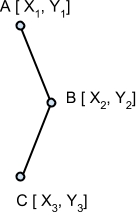
\includegraphics[height=100px]{punish}
\caption{Fragment �amanej jako toru przejazdu}
\label{fig:punish}
\end{figure}

\subsection{Strategia sumowania pochodnych}
\label{sec:strategiaPochodnych}

Pierwsza strategia opiera si� na obliczaniu kolejno przybli�enia drugich pochodnych funkcji za pomoc� iloraz�w r�nicowych w ka�dym kolejnym punkcie trasy a nast�pnie zsumowaniu ich bezwzgl�dnych warto�ci. 

\begin{equation}
\ddot{d_i} = \frac{x_1 + x_3 - 2x_2}{(y_3 -y_2) (y_2-y_1) }
\end{equation}

\begin{equation}
k =  \sum\limits_{i=1}^{n-1} |\ddot{d_i}|^{3} 
\end{equation}

Powsta�� liczb� $k$ mo�na traktowa� jako wsp�czynnik, kt�rego ma�a bezwzgl�dna warto�� oznacza bardzo �agodne k�ty przej�cia na ca�ej trasie natomiast im wi�ksz� ,,kanciasto��'' trasy tym wi�ksza warto�� tego wsp�czynnika. Dodatkowo, przed zsumowaniem, warto�� bezwzgl�dna przybli�onej drugiej pochodnej jest podnoszona do trzeciej pot�gi. Wyliczony wsp�czynnik dla ka�dej z rozwa�anych w algorytmie tras jest mno�ony przez obliczony czas przejazdu tej trasy. Dopiero taka liczba jest traktowana jako warto�� funkcji celu algorytmu genetycznego. Minusem tej strategii jest przeskalowanie realnego czasu przejazdu narciarza po zadanym torze, a zatem brak mo�liwo�ci por�wnania go do wynik�w uzyskiwanych innymi metodami.

\subsection{Strategia proporcjonalnego zmniejszania warto�ci wektora pr�dko�ci}
\label{sec:strategiaZmniejszania}

W tej strategii, dla ka�dego wierzcho�ka �amanej, obliczamy indywidualny wsp�czynnik kary $m$ z zakresu od 0 do 1. D�ugo�� wektora pr�dko�ci w ka�dym kolejnym punkcie b�dzie mno�ona przez wsp�czynnik dla tego punktu. Modelowane b�dzie zatem przyhamowywanie - tym wi�ksze, im wi�kszy jest k�t pomi�dzy kolejnymi punktami �amanej. Wsp�czynnik w danym punkcie zale�y od k�ta ABC z rysunku \ref{fig:punish} pomi�dzy poprzednim a nast�puj�cym punktem. Zaproponowana zosta�a nast�puj�ca funkcja, zmierzaj�ca do zera dla k�ta 90 stopni i mniejszego, i zmierzaj�ca do jedynki dla 180 stopni.


\begin{equation}
m\left(\alpha\right) = \left \{ {{0.01, \alpha \in \left( 0, 90\right)} \atop {1- \left(  \frac{\alpha}{180} - 1.5  \right)^{6}, \alpha \in \left[ 90, 180\right) }} \right.
\end{equation} 
  
 
\begin{figure}[h]
\centering
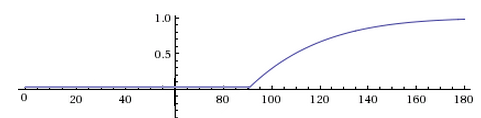
\includegraphics[height=70px]{punish-fun-1} 
\caption{Wykres funkcji}
\label{fig:punish} 
\end{figure}

\subsection{Strategia karania za ka�d� zmian� kraw�dzi}
\label{sec:strategiaKrawedzi}

Ostatnia strategia przyjmuje, �e nie ma potrzeby wykonywa� dodatkowych skr�t�w pomi�dzy bramkami. Cho� teoretycznie jest mo�liwe, by taki dodatkowy skr�t pozwala� uzyska� lepszy czas, to jednak jest to niespotykane podczas rzeczywistej jazdy po slalomach. Dlatego w strategii tej zlicza si� liczb� zmian kierunku jazdy na testowanym torze i por�wnuje j� z ilo�ci� bramek wymuszaj�cych skr�t na trasie. Otrzymujemy zatem liczb� nadmiarowych zmian kraw�dzi, kt�re w ka�dym przypadku powoduj� gorszy czas przejazdu ni� gdyby ich nie by�o. Aby to zatem zamodelowa�, w tej strategii dodajemy do wyliczonego czasu przejazdu sta�� liczb� sekund kary za ka�d� niepotrzebn� zmian� kraw�dzi i to traktujemy jako warto�� funkcji celu algorytmu ewolucyjnego.

%---------------------------------------------------------------------------

\section{Architektura systemu}
\label{sec:architektura}

Wyb�r docelowej architektury dla naszego systemu zosta� poprzedzony eksperymentowaniem z dwoma r�nymi, zgo�a odmiennymi podej�ciami. Dzi�ki temu, zosta�y przeanalizowane mocne i s�abe punkty ka�dej z nich, a ostatecznie wybrane rozwi�zanie spe�nia wszystkie potrzeby.

\subsection{Architektura prototypowa}

Pierwszym wybranym przez nas �rodowiskiem tworzenia systemu by� j�zyk Python i dost�pne dla niego modu�y: VPython umo�liwiaj�cy wizualizacj� w 2D i 3D oraz biblioteki numeryczne NumPy i SciPy wykorzystywane do rozwi�zywania r�wna� r�niczkowych. 

Dobrze znany nam j�zyk pozwoli� nam na szybkie prototypowanie i testowanie pierwszego fizycznego modelu narciarza. Wizualizacja by�a prosta w implementacji, a biblioteki numeryczne wystarczaj�co dobrze udokumentowane i powszechnie u�ywane, co zapewnia�o ich stabilno�� i jako��. Szybko ujawni�y si� jednak wady wybranego �rodowiska - uruchomienie naszego programu wymaga�o od u�ytkownika instalacji z�o�onego �rodowiska do obs�ugi j�zyka Python oraz graficznych i numerycznych bibliotek, co by�o istotn� barier�. Stanowi�o to powa�ny problem, bior�c pod uwag� potencjaln� mo�liwo�� rozpraszania oblicze�. Zda�y�my sobie spraw�, �e rozwi�zywany przez nas problem i otrzymywane przez nas wyniki s� atrakcyjne wizualnie i ludzie zwi�zani z narciarstwem z ch�ci� mog� wzi�� udzia� w obliczeniach i udost�pni� nam zasoby obliczeniowe swoich komputer�w. Wiedzia�y�my, �e warunkiem koniecznym by zrealizowa� t� wizj� jest �atwo�� w do��czaniu do oblicze�, wizualizacji wynik�w i bezproblemowa konfiguracja. Bior�c to pod uwag�, zdecydowa�y�my, �e potrzebujemy innego �rodowiska.

\subsection{Architektura docelowa}

Potrzeba �atwo�ci do��czania do oblicze� sk�oni�a nas do stworzenia systemu, w kt�rym klientami obliczeniowymi s� przegl�darki internetowe. Klienci chc�cy pod��czy� si� do oblicze� wchodz� na dobrze znany adres internetowy sk�d serwowana jest strona g��wna i skrypty, kt�re dokonuj� oblicze�. Na ��danie klienta, dostaje on ze zdalnego serwisu egzemplarz problemu, kt�ry jest nast�pnie lokalnie przetwarzany i wizualizowany klientowi na bie��co. Po sko�czonym obliczeniu, rozwi�zanie jest umieszczane na serwerze, a klient mo�e przej�� do obliczania kolejnego lub jeszcze raz tego samego problemu.

Architektura naszego systemu sk�ada si� z dw�ch g��wnych, niezale�nych cz�ci sk�adowych. Pierwsz� z cz�ci jest aplikacja kliencka przeprowadzaj�ca obliczenia i wizualizacj� oraz komunikuj�ca si� z serwerem zarz�dzaj�cym obliczeniami. Drugim jest aplikacja \textit{lekkiego} serwera http, jako warstwa wystawiaj�ca REST API. Warstw� persystentn� jest dokumentowa, nierelacyjna baza danych CouchDB. Schemat architektury prezentuje rysunek \ref{fig:architektureSimple}.

\begin{figure}[H]
\centering
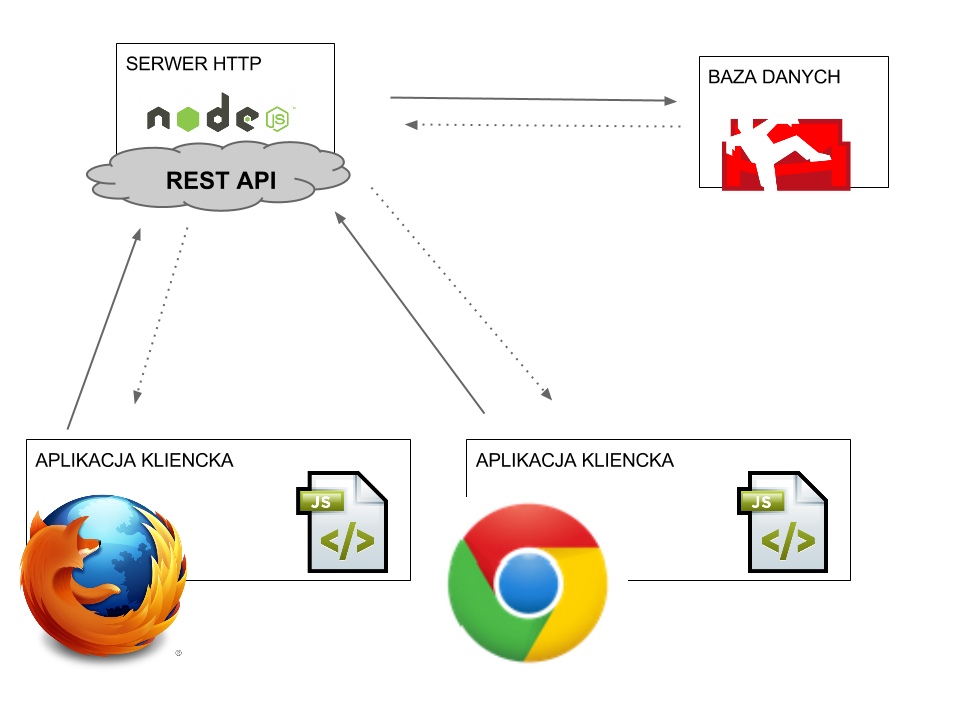
\includegraphics[width=360px]{architekture-simple}
\caption{Uproszczony schemat architektury docelowej}
\label{fig:architektureSimple}
\end{figure}


\subsection{Aplikacja kliencka}

Aplikacja kliencka to aplikacja webowa stworzona przy u�yciu frameworku Chaplin, wprowadzaj�cego dobre praktyki w strukturyzowaniu aplikacji Java Script'owych wykorzystuj�cych bibliotek� Backbone.js. Aplikacja w ca�o�ci napisana jest w j�zyku Coffee Script. Jest to j�zyk programowania ze sk�adni� podobn� do sk�adni Python'a, kompiluj�cy si� do Java Script'u. Powsta�y po kompilacji kod Java Script jest czytelny i przyjazny do debugowania. Programuj�c w Coffee Script mo�na u�ywa� wszystkich bibliotek i modu��w napisanych w Java Script, co daje wiele mo�liwo�ci z powodu szerokiego zakresu dost�pnych bibliotek w tym j�zyku. Zdecydowa�y�my si� u�ywa� tego j�zyka przede wszystkim z uwagi na sk�adni� przypominaj�c� dobrze znany nam j�zyk Python, wi�ksz� przejrzysto�� i czytelno�� kodu ni� Java Script, jednocze�nie zachowuj�c szerokie mo�liwo�ci tego j�zyka.

Aplikacja ma zasadniczo trzy warstwy:
\begin{itemize}
\item warstw� prezentacyjn� i wizualizacyjn� dla rozwi�zywanego problemu,
\item warstw� komunikacji z serwerem,
\item warstw� obliczeniow�.
\end{itemize}

\begin{figure}[h]
\centering
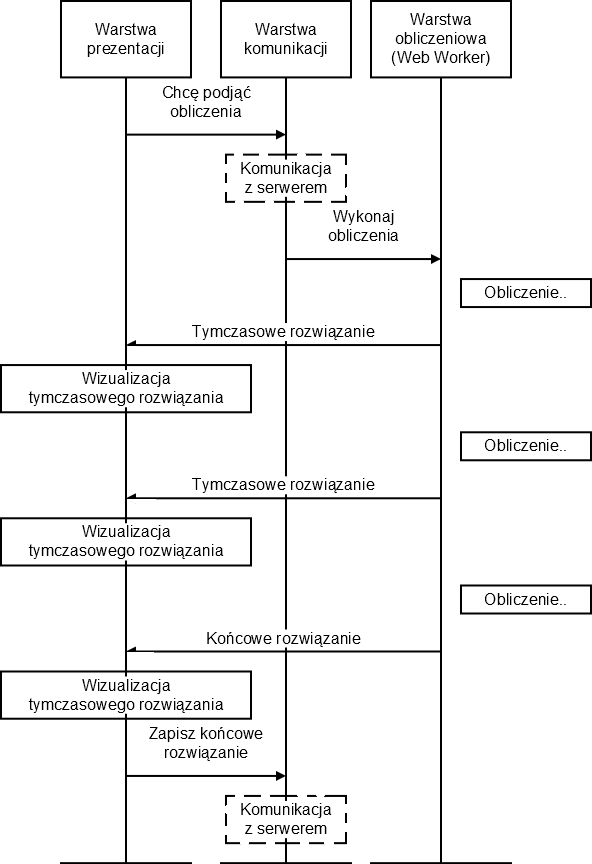
\includegraphics[width=360px]{diagramClientLayers}
\caption{Uproszczony diagram sekwencji pomi�dzy poszczeg�lnymi warstwami aplikacji klienckiej. Warstwa obliczeniowa przekazuje do warstwy prezentacji wiele tymczasowych rozwi�za� oraz, po zako�czeniu pe�nego cyklu oblicze�, finalne, najlepsze rozwi�zanie, kt�re nast�pnie przekazywane jest na serwer.}
\label{diagramClientLayers}
\end{figure}

Komunikacje pomi�dzy poszczeg�lnymi warstwami aplikacji klienckiej w postaci diagramu sekwencji przedstawia Diagram \ref{diagramClientLayers} na stronie \pageref{diagramClientLayers}.

\subsubsection{Warstwa prezentacji}

Wizualizacja zaimplementowana jest na elemencie Canvas ze specyfikacji HTML5. Wykresy wizualizuj�ce przebieg oblicze� stworzone s� przy u�yciu biblioteki Highcharts. Warstwa spe�nia nast�puj�ce funkcje:
\begin{itemize}
\item wyja�nienie u�ytkownikowi jaki problem jest rozwi�zywany oraz jak mo�e pom�c,
\item umo�liwienie rozpocz�cia wzi�cia udzia�u w obliczeniu,
\item prezentowanie trasy narciarskiej (uk�adu bramek), pobranej z serwera do oblicze�,
\item wizualizacja na bie��co wynik�w oblicze� w postaci rozwa�anego jako najlepszy toru przejazdu,
\item wizualizacja statystyk algorytmu obliczaj�cego w postaci wykres�w.
\end{itemize}

\subsubsection{Warstwa komunikacyjna}

Komunikacja z serwerem odbywa si� poprzez REST-owe API, wykorzystuj�ce JSON-owy format do wymiany danych. Warstwa spe�nia nast�puj�ce funkcje:
\begin{itemize}
\item pobieranie instancji problemu do obliczenia,
\item wysy�anie na serwer rozwi�zania zadanego problemu,
\item pobierania z serwera informacji o obecnie najlepszym rozwi�zaniu tego problemu.
\end{itemize}

\subsubsection{Warstwa obliczeniowa}

Zastosowanie w naszej architekturze Web Worker'�w do wykonywania oblicze� jest dobrze uzasadnione, bior�c pod uwag� ich specyfikacj�, opisan� szerzej w rozdziale \ref{webWorkers}. Obliczenia trasy przejazdu nawet dla toru z kilkoma bramkami zajmuje co najmniej kilka sekund. Worker na bie��co, w trakcie trwania oblicze�, przekazuje do g��wnego procesu obs�uguj�cego UI strony, kolejne rozwa�ane trasy. Proces UI rysuje na elemencie Canvas na bie��co otrzymywan� tras�.

\subsection{Aplikacja serwerowa}

Aplikacja jest lekkim serwerem Http napisanym w �rodowisku Node.js. U�ytym j�zykiem programowania, podobnie jak w aplikacji klienckiej, jest Coffee Script. Serwer wystawia REST-owe API, u�ywaj�c do wymiany danych JSON-owego formatu serializacji. Serwer komunikuje si� z dokumentow� baz� danych CouchDB. Podstawowymi funkcjami serwera s�:

\begin{itemize}
\item umo�liwienie dodania instancji problemu obliczeniowego do bazy danych,
\item zwracanie na ��danie problemu obliczeniowego do rozwi�zania,
\item zwracania informacji o obecnych dost�pnych rozwi�zaniach ka�dego z problem�w obliczeniowych.
\end{itemize} 

\begin{figure}[h]
\centering
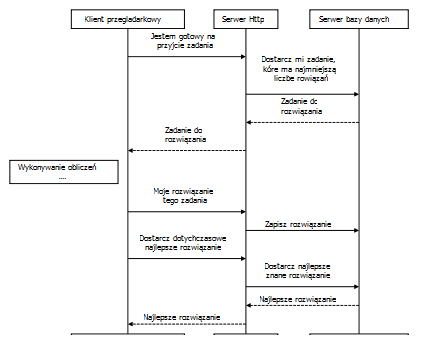
\includegraphics[width=360px]{diagramClientServerDb}
\caption{Uproszczony diagram sekwencji pomi�dzy poszczeg�lnymi komponentami systemu oraz warstw� persystencji}
\label{diagramClientServerDb}
\end{figure}

Diagram \ref{diagramClientServerDb} na stronie \pageref{diagramClientServerDb} pokazuje sekwencj� komunikacji pomi�dzy komponentami systemu oraz warstw� persystencji.

\subsection{Interfejs systemu udost�pniony u�ytkownikowi}

Efektem widocznym dla ko�cowego u�ytkownika powsta�ej na potrzeby tej pracy aplikacji jest strona www, dost�pna pod adresem URL - \textit{http://giant-client.herokuapp.com/}. Na stronie, poza kr�tkim wyt�umaczeniem celu projektu i sposobu w jaki ka�dy odwiedzaj�cy mo�e pom�c w obliczeniach, znajduje si� jedno wyra�ne tzw. ``call to action'' - du�y przycisk zach�caj�cy do rozpocz�cia oblicze�.

\begin{figure}[h]
\centering
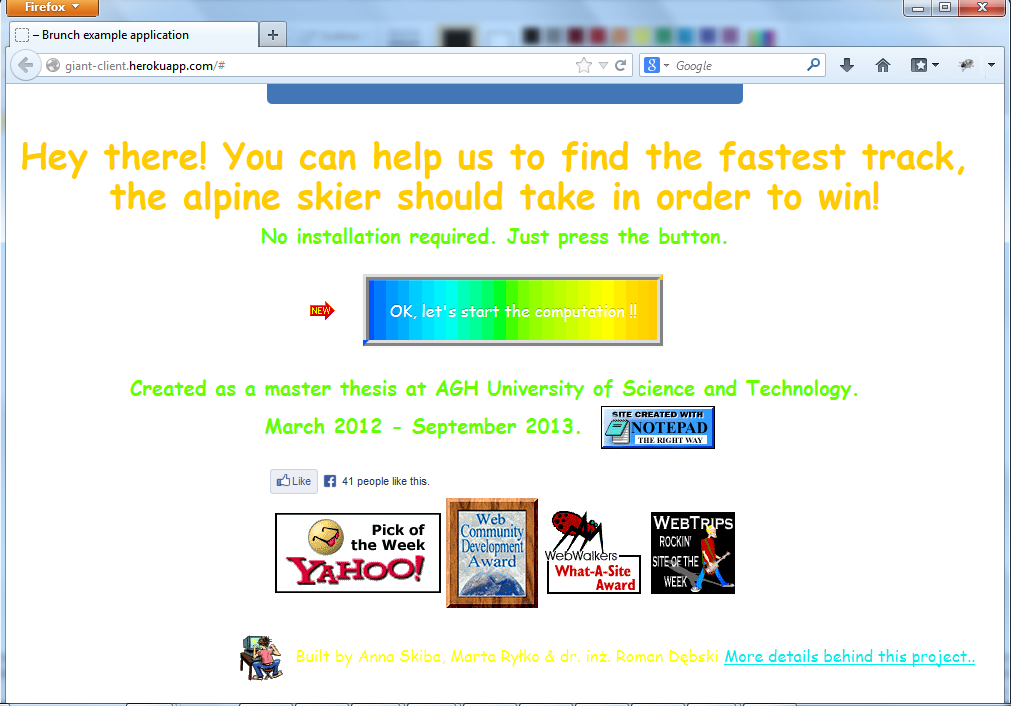
\includegraphics[width=400px]{interfejs-1}
\caption{Strona g��wna zach�caj�c� do uruchomienia oblicze�}
\label{fig:interfejs-1}
\end{figure}

Po uruchomieniu oblicze� osoba odwiedzaj�ca stron� dostaje na bie��co informacje zwrotne dotycz�ce efekt�w jej wsp�pracy. Na stronie:

\begin{itemize}
\item rysowana jest ca�y czas aktualnie rozwa�ana jako najlepsza trasa przejazdu,
\item wy�wietla si� obliczony czas przejazdu po aktualnie rozwa�anym torze przejazdu,
\item wy�wietla si� najlepszy, dotychczas znaleziony, czas przejazdu dla aktualnie rozwa�anej konfiguracji trasy,
\item rysowane s� wykresy przedstawiaj�ce statystyki algorytmu ewolucyjnego (aktualny Fitness populacji - najlepszy, najgorszy oraz �rednia dla wszystkich osobnik�w).
\end{itemize}

\begin{figure}[h]
\centering
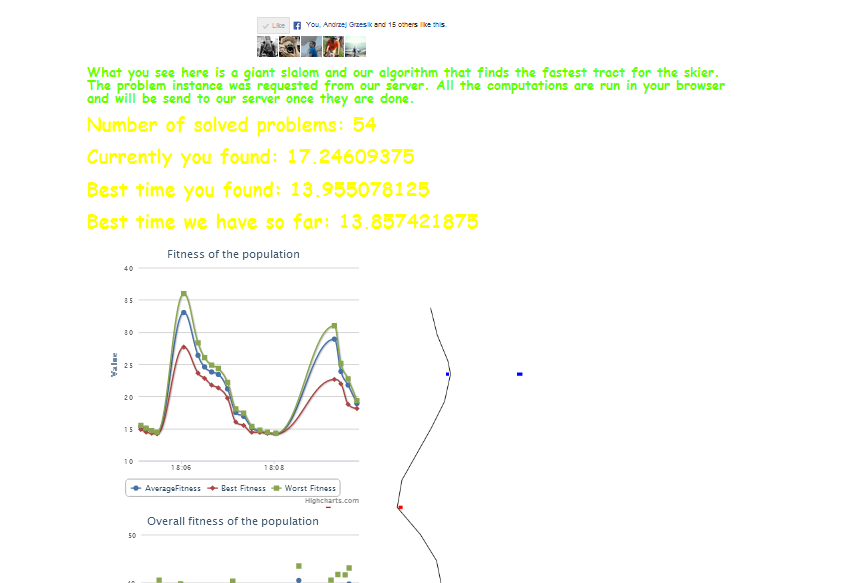
\includegraphics[width=500px]{interfejs-2}
\caption{Aplikacja w trakcie prowadzenia oblicze�}
\label{fig:interfejs-2}
\end{figure}

\chapter{Wyniki}
\label{cha:wyniki}

W rozdziale tym przedstawiono informacje na temat wynik�w przeprowadzonych eksperyment�w. Najpierw przedstawione zosta�y testy zar�wno teoretyczne, jak i w praktyce pokazuj�ce poprawno�� zastosowanego modelu. Nast�pnie pokazane zosta�y wyniki optymalizacji algorytmu ewolucyjnego, lokalnej optymalizacji oraz mechanizmu karania dla r�nych parametr�w. Na koniec om�wione zosta�y wyniki dotycz�ce zastosowanego rozwi�zania architektonicznego oraz skuteczno�ci Volunteer Computing.

Je�eli nie jest wskazane inaczej, w eksperymencie przyjmowane s� nast�puj�ce warto�ci sta�e:
\begin{itemize}
\item $\mu = 0.05$ - wsp�czynnik tarcia, typowa warto�� dla nasmarowanych nart
\item $\rho = 1.17 \frac{kg}{m^3}$ - przybli�ona warto�� g�sto�ci powietrza dla temperatury $0^\circ C$
i wilgotno�ci 20\% na wysoko�ci 800 m n.p.m
\item $C = 0.6$ - wsp�czynnik oporu powietrza, typowe warto�ci to 0.4 - 1
\item $A = 0.2 m^2$ - frontalna powierzchnia narciarza w projekcji prostopad�ej do wektora pr�dko�ci narciarza
\item $k_1 = 0.05 $ - wsp�czynnik oporu powietrza
\item $k_2 = \frac{1}{2}C \rho A$ - wsp�czynnik oporu powietrza
\end{itemize}
Opis powy�szych sta�ych mo�na znale�� w rozdzia�ach \ref{sec:fizycznyModel} oraz \ref{sec:ewolucyjny}.

W rozdziale zastosowano nast�puj�ce oznaczenia:
\begin{itemize}
\item ES - strategia ewolucyjna (w tym przypadku ($\mu$ + $\lambda$))
\item HC - Hill climbing
\item PF - funkcja kary
\end{itemize}

W eksperymentach wszystkie wsp�rz�dne punkt�w s� w uk�adzie kartezja�skim, dwuwymiarowym, zorientowanym na p�aszczy�nie stoku. O� x skierowana jest wzd�u� stoku, natomiast o� y w poprzek.
%---------------------------------------------------------------------------

%TODO biblio do artyku�u
\section{Weryfikacja modelu}
\label{sec:weryfikacja}

W tej sekcji chcia�y�my pokaza�, �e model, kt�ry zosta� przyj�ty jest prawid�owy. W poni�szych eksperymentach zostanie sprawdzone, czy zale�no�ci pomi�dzy zmian� poszczeg�lnych zmiennych modelu, takich jak masa, nachylenie stoku oraz opory ruchu, a otrzymywanym czasem przejazdu, s� zgodne z prawami fizyki. Kolejne eksperymenty zweryfikuj� r�wnie�, czy czas przejazdu po teoretycznie najszybszej trasie jest podobny do tego, kt�ry mo�na wyliczy� ze wzor�w przedstawionych w artyku�ach naukowych. Na koniec sprawdzimy czy mo�liwe jest przybli�anie jazdy narciarza jazd� po �amanej i jak g�sto b�d� musia�y by� rozmieszczane punkty przegi�cia, �eby nie straci� na dok�adno�ci wynik�w.

\subsection{Masa i nachylenie stoku}
Na pocz�tek zosta�y przeprowadzane proste eksperymenty, kt�re mia�y udowodni�, �e przyj�ty model jest prawid�owy. Dlatego dla cel�w pierwszego testu naj�atwiej by�o sprawdzi� jak zmienia si� czas przejazdu narciarza poruszaj�cego si� po prostej w d� stoku przy r�nych masach narciarza oraz zmianach nachylenia stoku, dodatkowo sprawdzaj�c jaki wp�yw na wyniki ma r�wnie� tarcie oraz op�r powietrza.

Przypomnijmy r�wnanie \ref{eq:rownRuchu}, kt�re opisuje model poruszania si� narciarza:

\begin{equation}
\label{eq:rownRuchu}
\ddot{x}=g\sin\alpha-\mu g\cos\alpha - \frac{k_2}{m}\dot{x}^2
\end{equation}

Zauwa�my, �e jego masa wp�ywa jedynie na warto�� przyspieszenia wynikaj�c� z si�y oporu powietrza. Natomiast k�t nachylenia $\alpha$ wp�ywa zar�wno na si�� �ci�gaj�c�, jak i na si�� tarcia. W opisanym eksperymencie zostanie pokazane, �e:
\begin{itemize}
\item im wi�kszy k�t nachylenia stoku tym szybciej porusza si� narciarz, bez wzgl�du na rodzaj uwzgl�dnionych si� oporu,
\item je�li uwzgl�dnimy tylko si�� �ci�gaj�c�, bez si� oporu, czas przejazdu narciarzy o r�nych masach na tej samej trasie jest identyczny,
\item taki sam wynik otrzymamy je�li uwzgl�dnimy dodatkowo si�� tarcia,
\item przy uwzgl�dnieniu si�y oporu powietrza otrzymujemy nast�puj�c� zale�no��: im wi�ksza jest masa narciarza, tym mniejsze jest op�nienie wynikaj�ce z si�y oporu powietrza, co skutkuje szybszym przejazdem narciarza (przy za�o�eniu, �e frontalna powierzchnia narciarza $A$ nie zmienia si�).
\end{itemize}

\subsubsection{Opis eksperymentu}
Eksperyment zosta� przeprowadzony na dw�ch modelach stok�w narciarskich. Oba maj� 600 m d�ugo�ci co odpowiada rzeczywistej d�ugo�ci stoku Harenda w Zakopanem. Stoki modelujemy jako r�wnie pochy�e o sta�ym nachyleniu. Aby zweryfikowa� dodatkowo prawid�owo�� modelu, w eksperymencie zosta�y wprowadzone rzeczywiste warto�ci nachyle� stok�w Harenda w Zakopanem oraz Kotelnica w Bia�ce Tatrza�skiej.
\begin{itemize}
\item Harenda - ok. $20^\circ$ (0.3367 radian�w)
\item Kotelnica - ok. $8^\circ$ (0.1470 radian�w)
\end{itemize}

Zosta�y przeprowadzone trzy pr�by, kt�rych wyniki mo�na zobaczy� odpowiednio na kolejnych wykresach \ref{fig:bezOporow}, \ref{fig:bezOporu}, \ref{fig:wszystkieOpory}. W pierwszej cz�ci eksperymentu uwzgl�dniamy tylko i wy��cznie si�� grawitacji, w drugiej dok�adamy wy��cznie si�� tarcia, natomiast w trzeciej uwzgl�dniamy wszystkie si�y oporu, a wi�c tak�e si�� oporu powietrza.

\newpage
\subsubsection{Rezultaty eksperymentu}

\begin{figure}[H]
\centering
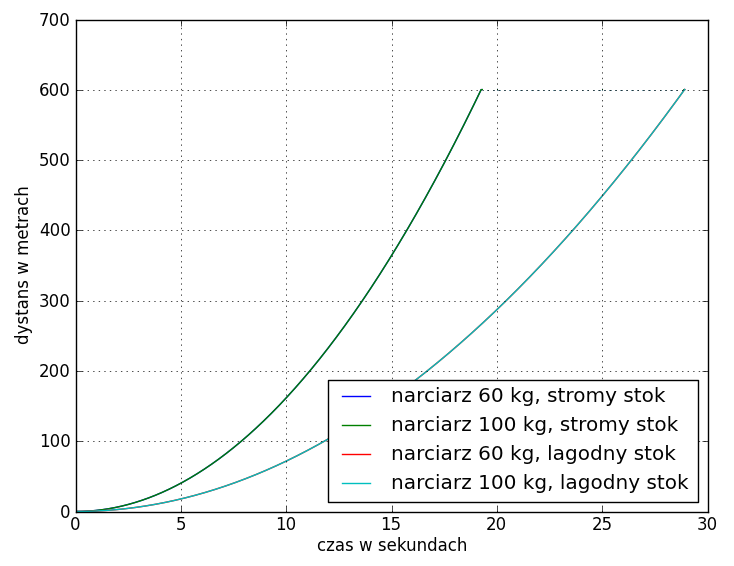
\includegraphics[scale=0.6]{experyment-masa-bez-oporow}
\caption{Por�wnanie czasu przejazdu narciarzy o r�nych masach, na stokach o r�nym nachyleniu bez uwzgl�dniania si� oporu. Linie wykres�w dla r�nych mas narciarzy i tego samego rodzaju stoku pokrywaj� si�.}
\label{fig:bezOporow}
\end{figure}

\begin{figure}[H]
\centering
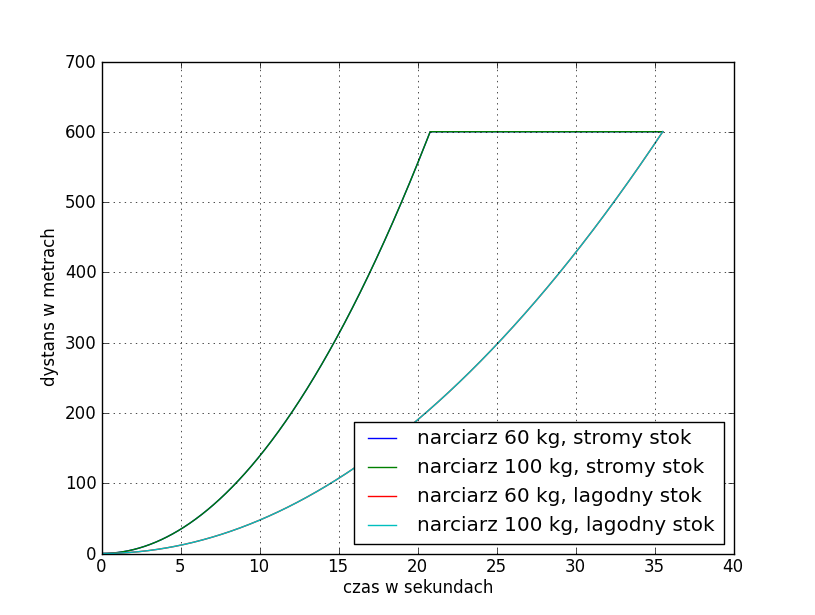
\includegraphics[scale=0.6]{experyment-masa-bez-oporu}
\caption{Por�wnanie czasu przejazdu narciarzy o r�nych masach, na stokach o r�nym nachyleniu z uwzgl�dnieniem si�y tarcia jako jedynej si�y oporu. Linie wykres�w dla r�nych mas narciarzy i tego samego rodzaju stoku pokrywaj� si�.}
\label{fig:bezOporu}
\end{figure}

\newpage
\begin{figure}[H]
\centering
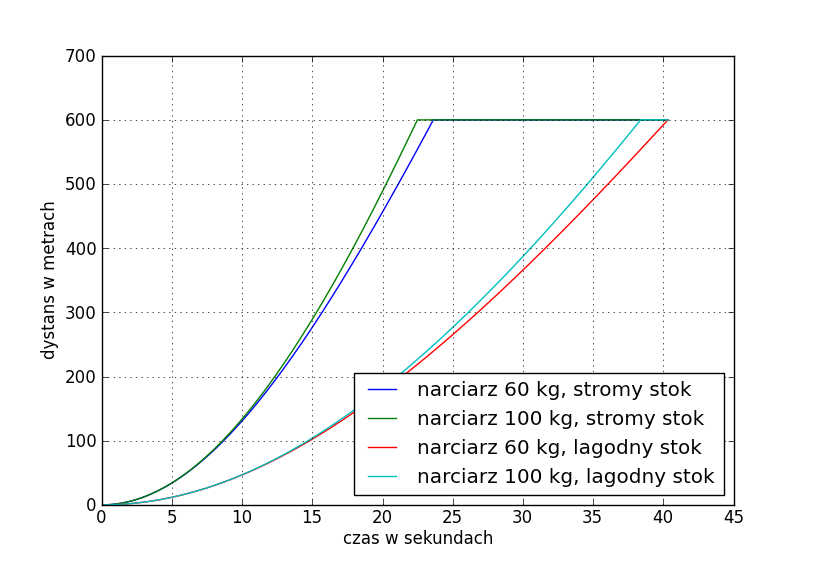
\includegraphics[scale=0.6]{experyment-masa}
\caption{Por�wnanie czasu przejazdu narciarzy o r�nych masach, na stokach o r�nym nachyleniu z uwzgl�dnieniem zar�wno si�y tarcia jak i oporu powietrza}
\label{fig:wszystkieOpory}
\end{figure}

Obserwujemy, �e w ka�dym z trzech przypadk�w na stromym stoku narciarze przeje�d�aj� ten sam dystans w kr�tszym czasie. W pierwszej i drugiej cz�ci eksperymentu nie ma znaczenia masa narciarza - czas przejazdu jest taki sam. Jednak na wykresie \ref{fig:bezOporow} czas przejazdu wynosi odpowiednio ok. 19 i 28 s., natomiast je�li uwzgl�dnimy si�� tarcia, czasy te wyd�u�aj� si� do ok. 21 i 35 s.\\
Analizuj�c wykres \ref{fig:wszystkieOpory} zauwa�amy, �e na bardziej stromym stoku r�nica w czasie przejazdu pomi�dzy ci�szym a l�ejszym narciarzem wynosi 1.14 s na korzy�� ci�szego, a na �agodniejszym 1.94 s r�wnie� na korzy�� ci�szego. Zmierzone czasy przejazdu slalomu w rzeczywisto�ci na stoku Harenda wynosz� ok. 40 s, a wi�c wydaje si� rozs�dne, �e przejazd na wprost mo�e zajmowa� ok. 22 s, kt�re zosta�y otrzymane w eksperymencie. W por�wnaniu z poprzednimi cz�ciami eksperymentu �atwo spostrzec, �e w ostatniej cz�ci czasy przejazdu s� d�u�sze - 22-23 oraz 38-40 s.

\subsection{Czas przejazdu w zale�no�ci od toru jazdy}
\label{sec:torJazdy}
Optymalizacja trasy narciarza polega na znalezieniu linii najszybszego przejazdu. Warto tu zauwa�y�, �e wbrew pozorom, nie zawsze jest to najkr�tsza linia - odcinek ��cz�cy punkt pocz�tkowy z ko�cowym. W poni�szym eksperymencie zostanie pokazane, jak zmienia si� czas przejazdu w zale�no�ci od linii poruszania si�.

Je�li rozwa�ymy przyk�ad bez bramek, gdzie najkr�tsza linia przejazdu nie powoduje jazdy w skos stoku, a jedynie w d�, to w takim przypadku, jest to jednocze�nie najszybsza trasa przejazdu. Jednak w pozosta�ych przypadkach, je�li rozwa�amy uk�ad bez dzia�ania opor�w, tory te b�d� r�ne.

\begin{figure}[H]
\centering
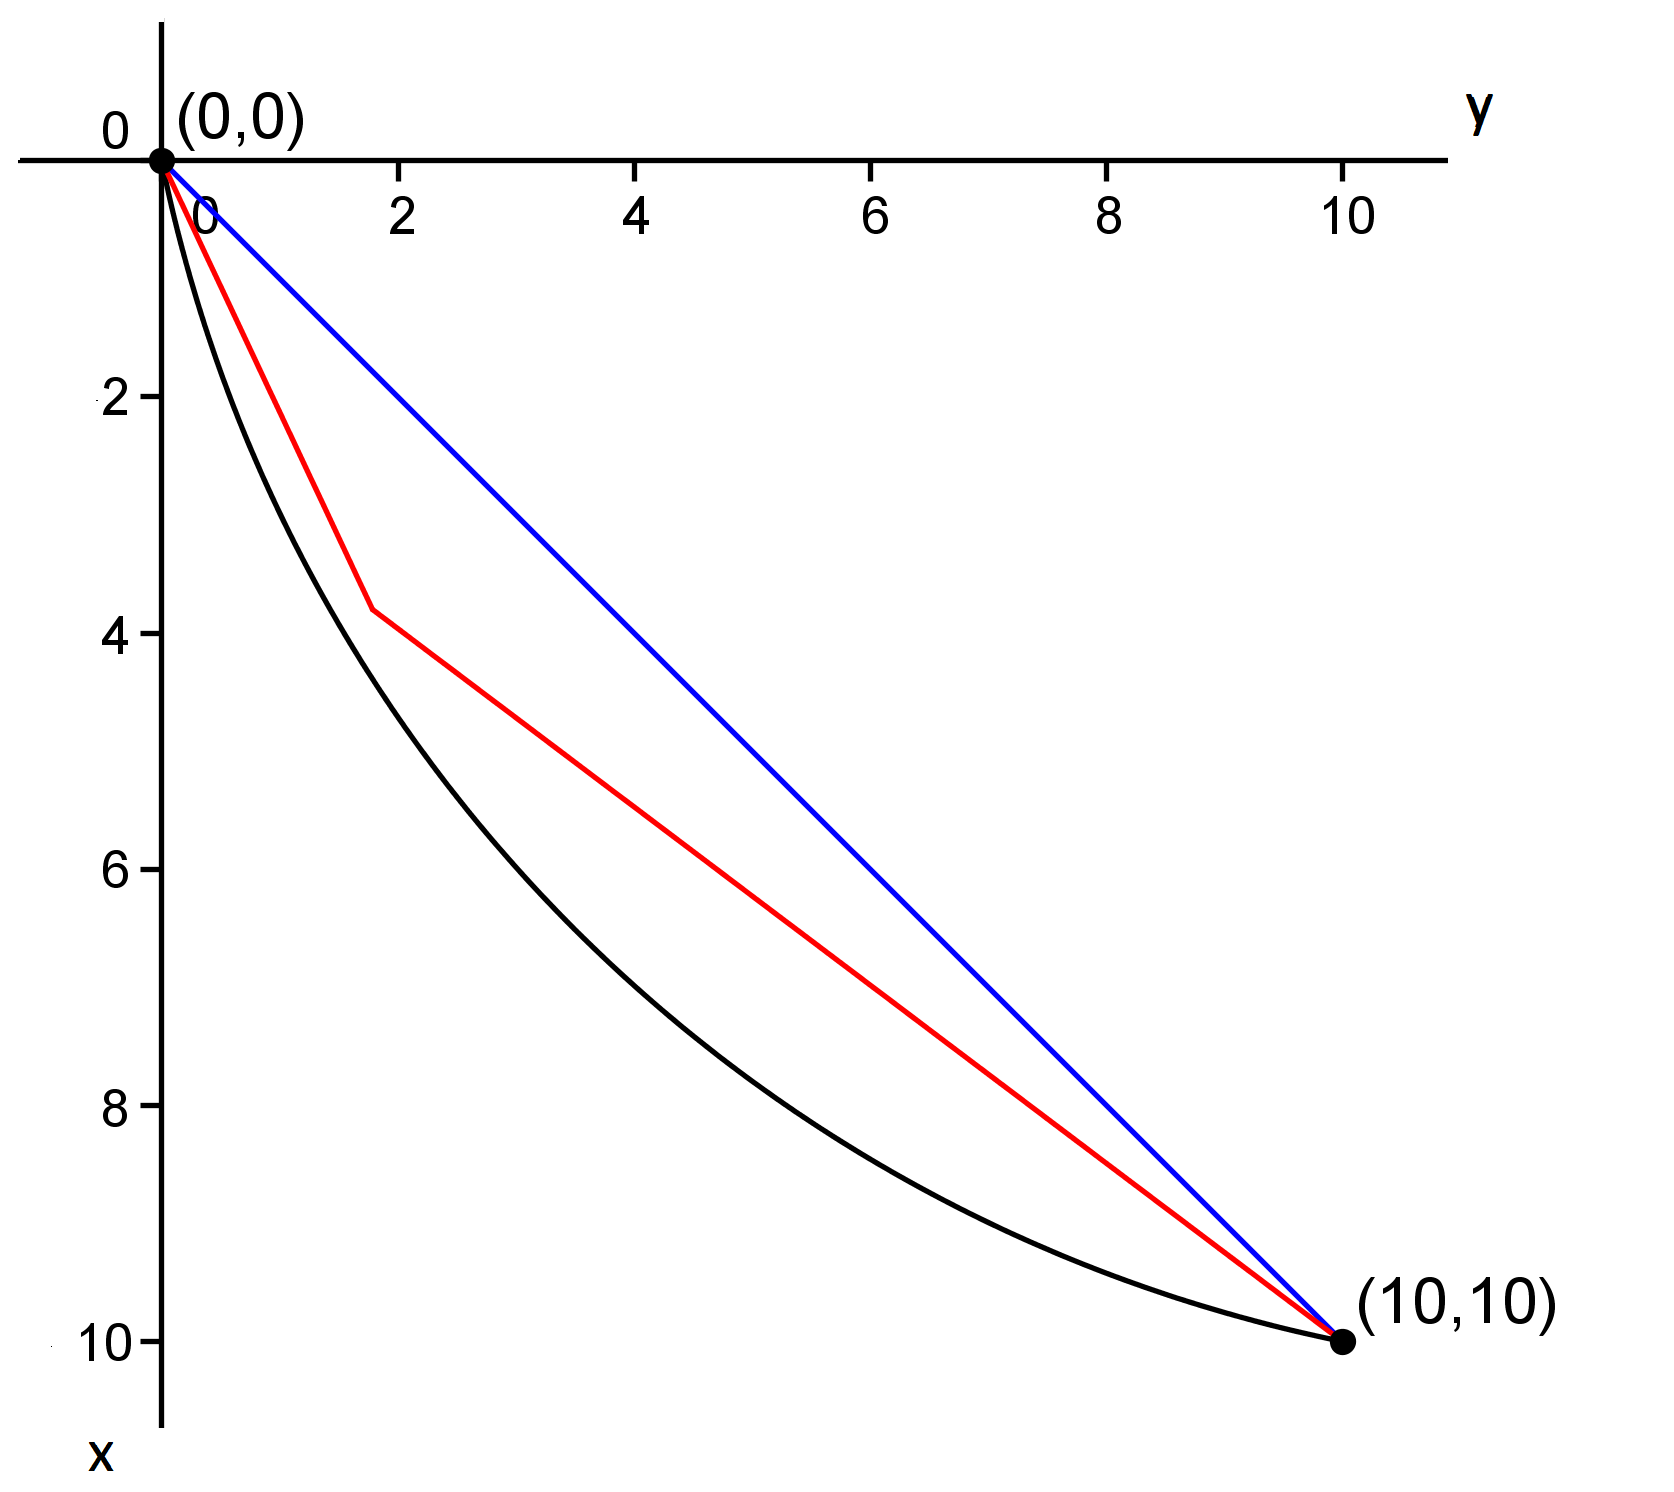
\includegraphics[scale=0.2]{trasy}
\caption{Przyk�adowe tory przejazdu od punktu (0,0) do punktu (10,10)}
\label{fig:trasy}
\end{figure}

\subsubsection{Opis eksperymentu}
Chcemy sprawdzi�, ile czasu zajmie narciarzowi przejechanie z punktu (0,0) do punktu (10,10). Na rysunku \ref{fig:trasy} pokazane s� przyk�adowe trasy przejazdu pomi�dzy tymi punktami. Aby upro�ci� eksperyment, sprawdzimy wyniki pomijaj�c wk�ad wszystkich opor�w. Gdyby narciarz porusza� si� po linii prostej, bezpo�rednio do punktu ko�cowego, czas przejazdu mo�na wyliczy� przekszta�caj�c wz�r:

\begin{equation}
s = \frac{at^2}{2}
\end{equation}

i otrzymuj�c:

\begin{equation}
t = \sqrt{\frac{2s}{a}}
\end{equation}

gdzie:
\begin{itemize}
\item $s = 10\sqrt{2}$ - odleg�o�� mi�dzy punktem pocz�tkowym i ko�cowym
\item $a = g\sin(\frac{\pi}{12})\sin(\frac{\pi}{4})$ - przyspieszenie narciarza
\end{itemize}
Przyspieszenie narciarza jest sk�adow� przyspieszenia ziemskiego uwzgl�dniaj�c� zar�wno nachylenie stoku ($\frac{\pi}{12}$), jak i jazd� w skos stoku ($\frac{\pi}{4}$, czyli $45^\circ$). Zatem, przyjmuj�c $g=9.81$, czas przejazdu po linii prostej powinien wynosi� oko�o:

\begin{equation}
t \simeq \sqrt{\frac{2*10\sqrt{2}}{9.81*\sin(\frac{\pi}{12})\sin(\frac{\pi}{4})}} \simeq 3.969 
\end{equation}

Sprawdzimy teraz jakie czasy otrzymamy wykorzystuj�c program, sprawdzaj�c poruszanie si� po linii prostej oraz po �wiartce okr�gu (a dok�adniej, po �amanej, kt�rej kolejne punkty za�amania znajduj� si� na okr�gu w niewielkich odleg�o�ciach od siebie). Poni�ej na rysunku \ref{fig:czasPrzejazdu} widzimy jak wygl�da trasa przejazdu w dw�ch przypadkach.

\begin{figure}[H]
\centering
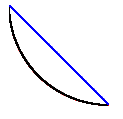
\includegraphics{czasPrzejazdu}
\caption{Tory przejazdu w eksperymencie por�wnuj�cym czas przejazdu dla r�nych linii jazdy}
\label{fig:czasPrzejazdu}
\end{figure}

\subsubsection{Rezultaty eksperymentu}
W tym przypadku otrzymali�my wyniki odpowiednio dla narciarza jad�cego po prostej 3.965 s, a dla poruszaj�cego si� po czarnej linii 3.671 s.

Po pierwsze, warto zwr�ci� uwag�, �e czas jazdy po prostej minimalnie r�ni si� od czasu teoretycznego, obliczonego ze wzoru - r�nica ta wynosi ok. 0.1\%, co jest dopuszczalne i mo�liwe do zaniedbania, gdy� nie ma znacz�cego wp�ywu na wyniki eksperyment�w. R�nica ta wynika z niedok�adno�ci oblicze� numerycznych. Dodatkowym problemem jest fakt, �e nie mo�emy wyliczy� dok�adnego czasu potrzebnego narciarzowi na dojechanie do okre�lonego punktu - mo�emy jedynie pr�bowa� zbli�a� si� do punktu ko�cowego, robi�c coraz mniejsze ``kroki'', staraj�c si� znale�� jak najbli�ej niego.

Wyra�nie wida� r�wnie�, �e czas przejazdu po linii czarnej jest kr�tszy ni� czas przejazdu po linii niebieskiej. Tras� po prostej narciarz przebywa w ok. 7\% d�u�szym czasie ni� tras� d�u�sz�. Na tak kr�tkim odcinku narciarz by� w stanie zdoby� przewag� ok. 0.3 s. Wa�ne jest to, �e w prawdziwych przejazdach slalomowych nawet najmniejsza r�nica czasu mo�e decydowa� o wygranej, oczywi�cie zale�y to od dok�adno�ci pomiaru, kt�ry zawsze jest sprawdzany do setnych cz�ci sekundy. Dlatego ogromne znaczenie ma tor po jakim porusza si� narciarz i nawet najmniejsza zmiana mo�e powodowa� kluczow� popraw� czasu na ca�ej trasie. Czasami warto jednak pojecha� d�u�sz� tras�, ale tak�, na kt�rej nabierzemy wi�kszej pr�dko�ci i p�niej zyskamy na kolejnym odcinku.

Pozostaje jeszcze pytanie, jaka jest najlepsza linia poruszania si� pomi�dzy dwoma punktami. Problem ten zosta� ju� rozwi�zany - linia najszybsza jest fragmentem cykloidy. Dok�adniejsze informacje mo�na znale�� m.in. w \cite{brach1} oraz \cite{brach2}. W \cite{brach2} znajduje si� wz�r na czas przejazdu pomi�dzy dwoma punktami. Korzystaj�c z tego wzoru, podstawiaj�c odpowiednio wyliczone parametry otrzymujemy, �e najkr�tszy mo�liwy czas przejazdu z punktu (0,0) do punktu (10,10) to ok. 3.623 s. Jak wida�, wynik ten jest lepszy ni� otrzymane w naszym eksperymencie: od czasu jazdy po �wiartce ko�a o ok. 0.05 s., co nie jest r�nic� bardzo du��, ale znacz�c� dla zwyci�stwa.

\subsection{Jazda po �amanej}
\label{sec:lamana}
Kolejnym krokiem by�o sprawdzenie, �e rzeczywi�cie mo�emy przybli�a� jazd� narciarza jako poruszanie si� po �amanej. Wa�ne jest stwierdzenie jakie r�nice w czasie b�d� wyst�powa� pomi�dzy jazd� po �uku, a jazd� po �amanej. R�nice te oczywi�cie b�d� zale�e� od tego, z ilu segment�w sk�ada� si� b�dzie �amana.

\subsubsection{Opis eksperymentu}
W eksperymencie sprawdza� b�dziemy jak zmienia si� czas przejazdu w zale�no�ci od dok�adno�ci przybli�enia �amanej. Jako tor przejazdu przyj�ta zosta�a najszybsza linia przejazdu do punktu (10,10), po kt�rej przejechanie zajmuje 3.623 s (jak wspomniano w poprzednim eksperymencie \ref{sec:torJazdy}).

Wybieraj�c okre�lon� liczb� punkt�w znajduj�cych si� na linii �uku sprawdzimy, ile czasu zajmuje przejechanie po �amanej utworzonej z tych punkt�w w por�wnaniu z jazd� po �uku. Nale�y r�wnie� okre�li�, jak g�sto musz� znajdowa� si� punkty, aby r�nica w czasie by�a zaniedbywalnie ma�a. Sterowanie odbywa si� poprzez ustalenie w jakiej odleg�o�ci od siebie w pionie maj� znajdowa� si� kolejne punkty - w ten spos�b r�wnie� mo�emy sterowa� liczb� punkt�w.

\subsubsection{Rezultaty eksperymentu}

Poni�ej znajduj� si� obrazki (Rysunek \ref{fig:brachSteps}) przedstawiaj�ce poszczeg�lne pr�by przejazdu po �amanej sk�adaj�cej si� odpowiednio z 2-6 punkt�w po�rednich (linia szara) oraz pierwotn� lini� najszybszego przejazdu (linia niebieska). Liczba punkt�w na �amanej nie bierze pod uwag� punktu startowego, a jedynie kolejne punkty w��cznie z punktem na mecie.

\begin{figure}[hp]
\centering

\includegraphics[scale=0.8]{brach_steps}
\caption{Linie przejazdu w poszczeg�lnych eksperymentach. Linia niebieska to najszybsza linia przejazdu, linia szara to �amana przybli�aj�ca lini� niebiesk�}
\label{fig:brachSteps}
\end{figure}

W tabeli \ref{tab:punktyPrzelamania} przedstawione s� uzyskane wyniki w zale�no�ci od ilo�ci punkt�w po�rednich oraz r�nica czasu w por�wnaniu do najkr�tszego czasu przejazdu - 3.623 s.

\begin{table}[h]
\caption{Czasy przejazdu po �amanej w zale�no�ci od liczby punkt�w prze�amania}
\centering
\label{tab:punktyPrzelamania}
\begin{tabular}{ | c | c | c |}
  \hline                        
  ilo�� punkt�w po�rednich & czas przejazdu [s] & r�nica w stosunku do czasu najszybszego [s] \\ \hline  
  2 & 3.687 & 0.064 \\ \hline
  3 & 3.647 & 0.023 \\ \hline
  4 & 3.635 & 0.012 \\ \hline
  5 & 3.629 & 0.006 \\ \hline
  6 & 3.626 & 0.003 \\ \hline
\end{tabular}
\end{table}

R�nice w czasie wahaj� si� od 0.003 do 0.064 s, jest to odpowiednio od 0.08\% do ok. 1.8\% r�nicy w stosunku do czasu najszybszego. Wydaje si�, �e wystarczaj�cym powinno by�, aby na odcinku takiej d�ugo�ci okre�li� trzy punkty po�rednie, gdy� r�nica dla tego przypadku wynosi ok. 0.023 s co stanowi ok. 100.6\% czasu najszybszego, a wi�c r�nica nie przekracza 1\%. To samo mo�na stwierdzi� z rysunk�w - ju� dla trzech punkt�w praktycznie nie wida� r�nicy pomi�dzy liniami. Zatem na takiej trasie, kt�rej odleg�o�� w pionie wynosi 10 m mo�na okre�li� 3-4 punkt�w po�rednich, kt�re z przybli�eniem nie wnosz�cym zbyt du�ych r�nic do wyniku b�d� wyznacza�y tras� ko�cow�. Oznacza to, �e punkty te powinny znajdowa� si� w odleg�o�ciach 2-4 m. Wiedz�c, �e pomiary przejazdu na zawodach s� z dok�adno�ci� do setnych cz�ci sekundy, mo�na stwierdzi�, �e dopiero 5 punkt�w po�rednich daje nam a� tak� precyzj� oblicze�. Oczywi�cie je�li trasa nie b�dzie zawiera� zbyt ostrych k�t�w za�amania, mo�na b�dzie zmniejszy� g�sto�� punkt�w.

\section{Eksperymenty w terenie}
\label{sec:eksperymenty}

Zainteresowanie tematyk� narciarsk�, sk�oni�o autorki pracy do przetestowania w terenie pewnych zale�no�ci i zjawisk opisywanych w tym rozdziale. Dzi�ki �yczliwo�ci Studenckiego Klubu Narciarskiego FIRN dzia�aj�cego na Akademii G�rniczo-Hutniczej w Krakowie, by�a mo�liwo�� dokonania pomiar�w przy u�yciu specjalistycznego sprz�tu do pomiaru czasu na stoku narciarskim. Zosta�y ustalone nast�puj�ce cele eksperyment�w:

\begin{itemize}
\item eksperymentalne wyznaczenie wsp�czynnika tarcia statycznego mi�dzy �niegiem a �lizgiem nart w zale�no�ci od sposobu nasmarowania �lizgu narty oraz jako�ci �lizgu,
\item eksperymentalne por�wnanie wp�ywu powierzchni narciarza na uzyskiwane czasy przejazdu, poprzez testowanie r�nych pozycji przejazdu oraz r�nych rodzaj�w odzie�y wierzchniej,
\item pr�ba por�wnania szybko�ci przejazdu z punktu A do B w linii prostej do jazdy po �uku.
\end{itemize} 

\subsection{Wsp�czynnik tarcia}
\label{subsec:espolczynnikTarcia}

\paragraph{Za�o�enia i warunki eksperymentu} 
W celu zmierzenia wsp�czynnika tarcia, zosta�a wykorzystana drewniana deska, kt�ra zosta�a przykryta warstw� ubitego, mokrego, marcowego �niegu. Przygotowane zosta�y cztery pary nart:
\begin{itemize}
\item \textbf{A} - Narta \textit{Atomic SL 11}, 150 cm d�ugo�ci, stary, nieprzygotowany i bardzo przesuszony �lizg.
\item \textbf{B} - Narta \textit{Head Worldcup Rebel S}, 155 cm d�ugo�ci, bardzo dobrze przygotowany �lizg, nasmarowany na gor�co niefluorowym smarem uniwersalnym (Toko System 3) 
\item \textbf{C} - Narta \textit{V�lkl Racetiger GS}, 175 cm d�ugo�ci, nowy, bardzo dobrze przygotowany pod zawody �lizg. �lizg by� posmarowany mi�dzy innymi smarami fluorowymi.
\item \textbf{D} - Narta \textit{Atomic Race GS 12}, 175 cm d�ugo�ci, stary, nieprzygotowany, jednak nie do ko�ca przesuszony �lizg
\end{itemize}

�lizg ka�dej narty przed eksperymentem by� wycierany, ale i tak by�o na nim osadzonych kilka kropel stopionego �niegu. Wy�o�ona ubitym �niegiem deska o d�ugo�ci oko�o 2.5 metra zosta�a z jednej strony podparta o pod�o�e, pozostaj�c pod niewielkim k�tem w stosunku do niego. Na desce odmierzono 2 metry od punktu podparcia i oznaczono ten punkt.

\begin{figure}[H]
\centering
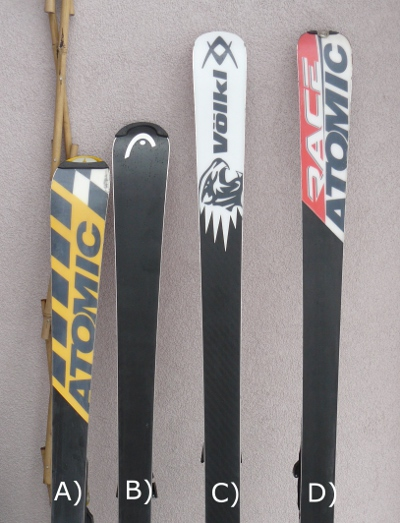
\includegraphics[height=300px]{narty}
\caption{Narty bior�ce udzia� w eksperymencie. Oznaczenia s� u�ywane w dalszej cz�ci opisu}
\label{fig:narty}
\end{figure}

\paragraph{Przebieg eksperymentu dla ka�dej z nart}
\begin{itemize}
\item wyznaczany by� �rodek ci�ko�ci narty i oznaczany markerem,
\item na desce k�adziona by�a narta, tak, by �rodek ci�ko�ci znajdowa� si� w oznaczonym wcze�niej punkcie odleg�ym o 2 metry od punktu podparcia,
\item stopniowo zwi�kszany by� k�t nachylenia deski do pod�o�a, a� do momentu w kt�rym narta straci�a przyczepno�� i zaczyna�a zsuwa� si� po �niegu,
\item mierzona by�a wysoko�� w linii prostej mi�dzy pod�o�em a punktem gdzie znajdowa� si� �rodek ci�ko�ci narty.
\end{itemize}

Dla ka�dej z nart przeprowadzone zosta�y dwie pr�by i jako wynik traktowana by�a �rednia z tych pr�b. Eksperyment mia� cel pozyskania wyniku podgl�dowego, dlatego te� liczba dw�ch pr�b zosta�a uznana za wystarczaj�c�. Jako, �e zauwa�ony zosta� podczas eksperymentu ogromny wp�yw wilgotno�ci �lizgu na wynik, zasta�y r�wnie� przeprowadzone pr�by dla dw�ch rodzaj�w nart z niewytartym �lizgiem, na kt�rym zebrana by�a znaczna ilo�� wody.

\paragraph{Wyniki i Wnioski}

\begin{figure}[H] 
\centering
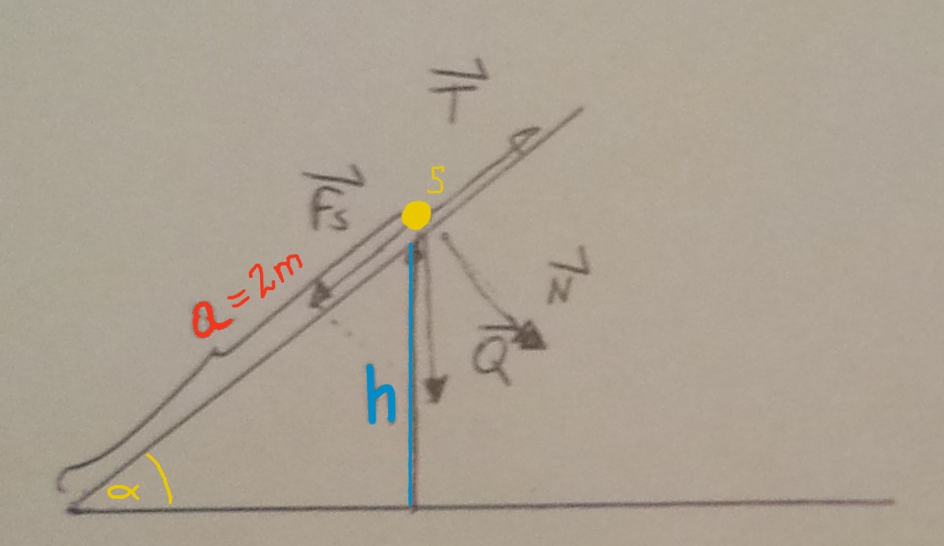
\includegraphics[height=160px]{rownia} 
\caption{S - �rodek ci�ko�ci narty; a - odleg�o�� mi�dzy �rodkiem ci�ko�ci narty a punktem podparcia deski; h - zmierzona eksperymentalnie wysoko�� graniczna, po przekroczeniu kt�rej narta zacz�a si� zsuwa� }
\label{fig:rownia}
\end{figure}

Aby obliczy� wsp�czynnik tarcia wykorzystana zosta�a nast�puj�ca zale�no��: dop�ki narta pozostaje w spoczynku oznacza to, �e si�a tarcia r�wnowa�y si�� �ci�gaj�c� dzia�aj�c� na cia�o. Zatem b�d�c na granicy zsuwania si�, tarcie statyczne osi�ga swoj� maksymaln� warto��. Zatem:

\begin{equation}
T = F_s
\end{equation}

\begin{equation}
 \mu Q\cos\alpha = Q\sin\alpha
\end{equation}

\begin{equation}
 \mu\cos\alpha = \sin\alpha
\end{equation}

\begin{equation}
 \mu = \tan\alpha 
\end{equation}

\begin{equation}
 \tan\alpha = \frac{\sin\alpha}{\sqrt{1-\sin\alpha}}
\end{equation}

\begin{equation}
 \sin\alpha = \frac{h}{a}
\end{equation}

\begin{equation}
 \mu = \frac{ \frac{h}{a}}{\sqrt{1- \frac{h}{a}}}
\end{equation}

W eksperymencie d�ugo�� $a$ by�a sta�a i zawsze wynosi�a 2 metry. Wyniki pomiar�w oraz obliczone warto�ci znajduj� si� w tabeli \ref{tab:wspolczynnikTarcia}. 

Wyniki okaza�y si� by� zgodne z przewidywaniami. Jako�� �lizgu, stan jego przegotowania oraz rodzaj smaru maj� znacz�cy wp�yw na warto�� wsp�czynnika tarcia, a w konsekwencji na szybko�ci poruszania si� na nartach. Ciekawym wnioskiem by�o to, �e mokry �lizg ma znacznie wi�kszy wsp�czynnik tarcia ni� suchy �lizg. Wychodzi zatem jak wa�na jest odpowiednio na�o�ona na �lizg struktura umo�liwiaj�ca odp�yw wody. Narta B mia�a �wie�� struktur�, podczas gdy narta D prawie jej nie mia�a. 

Jak wida�, wyliczone eksperymentalne wsp�czynniki tarcia dla niezawilgoconych �lizg�w mieszcz� si� w przedziale 0.125 - 0.193, przedzia� ten zawiera si� w przedziale 0.001 - 0.3 podanym we wst�pie teoretycznym w sekcji \ref{sec:tarcieKinetyczne} na stronie \pageref{sec:tarcieKinetyczne}.

\begin{table}[h]
\caption{Wyniki eksperymentu na wsp�czynnik tarcia w zale�no�ci od rodzaju �lizgu} 
\label{tab:wspolczynnikTarcia} 
\centering
\begin{tabular}{|c|c|c|c|c|c|}
\hline 
                                                                                                                         &                                                                    & \textbf{Narta A}                               & \textbf{Narta B} & \textbf{Narta C} & \textbf{Narta D} \\ \hline
\multirow{2}{*}{\textbf{\begin{tabular}[c]{@{}c@{}}wysoko��\\ na kt�rej zacz�o si�\\  osuwanie w metrach\end{tabular}}} & \textbf{\begin{tabular}[c]{@{}c@{}}osuszony \\ �lizg\end{tabular}} & 0.35& 0.26             & 0.235            & 0.28             \\ \cline{2-6} 
\multicolumn{1}{|l|}{\textbf{}}                                                                                          & \textbf{\begin{tabular}[c]{@{}c@{}}wilgotny \\ �lizg\end{tabular}} & ---                                            & 0.54             & ---              & 0.66             \\ \hline
\multirow{2}{*}{\textbf{wsp�czynnik tarcia}}                                                                            & \textbf{\begin{tabular}[c]{@{}c@{}}osuszony \\ �lizg\end{tabular}} & 0.193                                        & 0.139          & 0.125          & 0.151          \\ \cline{2-6} 
\multicolumn{1}{|l|}{\textbf{}}                                                                                          & \textbf{\begin{tabular}[c]{@{}c@{}}wilgotny\\  �lizg\end{tabular}} & ---                                            & 0.316          & ---              & 0.403         \\ \hline
\end{tabular}
\end{table}
 
\begin{figure}[H] 
\centering
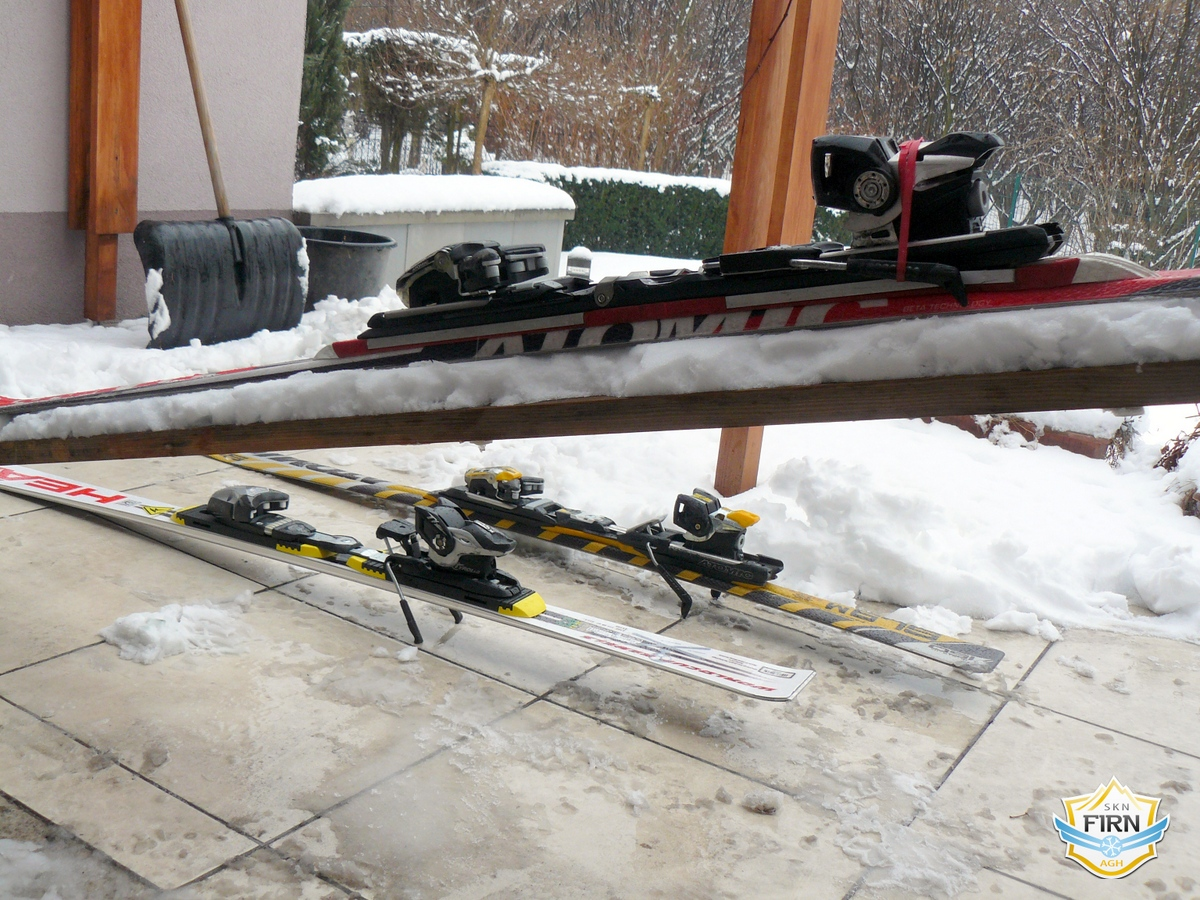
\includegraphics[height=220px]{eksp-1}
\caption{Warunki przeprowadzania eksperymentu. Wida� desk� z ubit� warstw� �niegu oraz u�o�on� na niej nart�}
\label{fig:eksp-1}
\end{figure}

\paragraph{Eksperymenty w ruchu}

Przeprowadzone zosta�y dodatkowo eksperymenty na stoku narciarskim. Pierwszy z nich polega� na por�wnaniu czas�w przejazdu w linii spadku stoku tego samego narciarza w nast�puj�cych niezmiennych warunkach:
\begin{itemize}
\item na odcinku o d�ugo�ci 28 metr�w, w linii spadku stoku, 
\item stoku o sta�ym nachyleniu oko�o $8^\circ$,
\item narciarz rozpoczyna przejazd bez odpychania si� kijami,
\item narciarz porusza si� po wyje�d�onym torze (brak �wie�ego �niegu),
\item narciarz ma ten sam str�j (kurtka narciarska i spodnie narciarskie) i pokonuje tras� w takiej samej pozycji - pozycji zr�wnowa�onej).
\end{itemize}

Warunkami zmiennymi eksperymentu by�y u�yte narty
\begin{itemize}
\item nieprzygotowane narty A,
\item bardzo dobrze przygotowane narty B,
\end{itemize}

Pomiar pr�dko�ci by� dokonywany przy u�yciu sprz�tu o dok�adno�ci co do setnej cz�ci sekundy. Sprz�t sk�ada si� z bramki startowej, kt�r� narciarz przekracza, uruchamiaj�c zegar. Zegar jest wy��czany automatycznie, gdy narciarz przetnie laserowy promie� przeprowadzony wzd�u� mety. Zegar u�ywany w eksperymencie mo�na zobaczy� na rysunku \ref{fig:eksp-3} na stronie \pageref{fig:eksp-3}.

\begin{figure}[H]
\centering
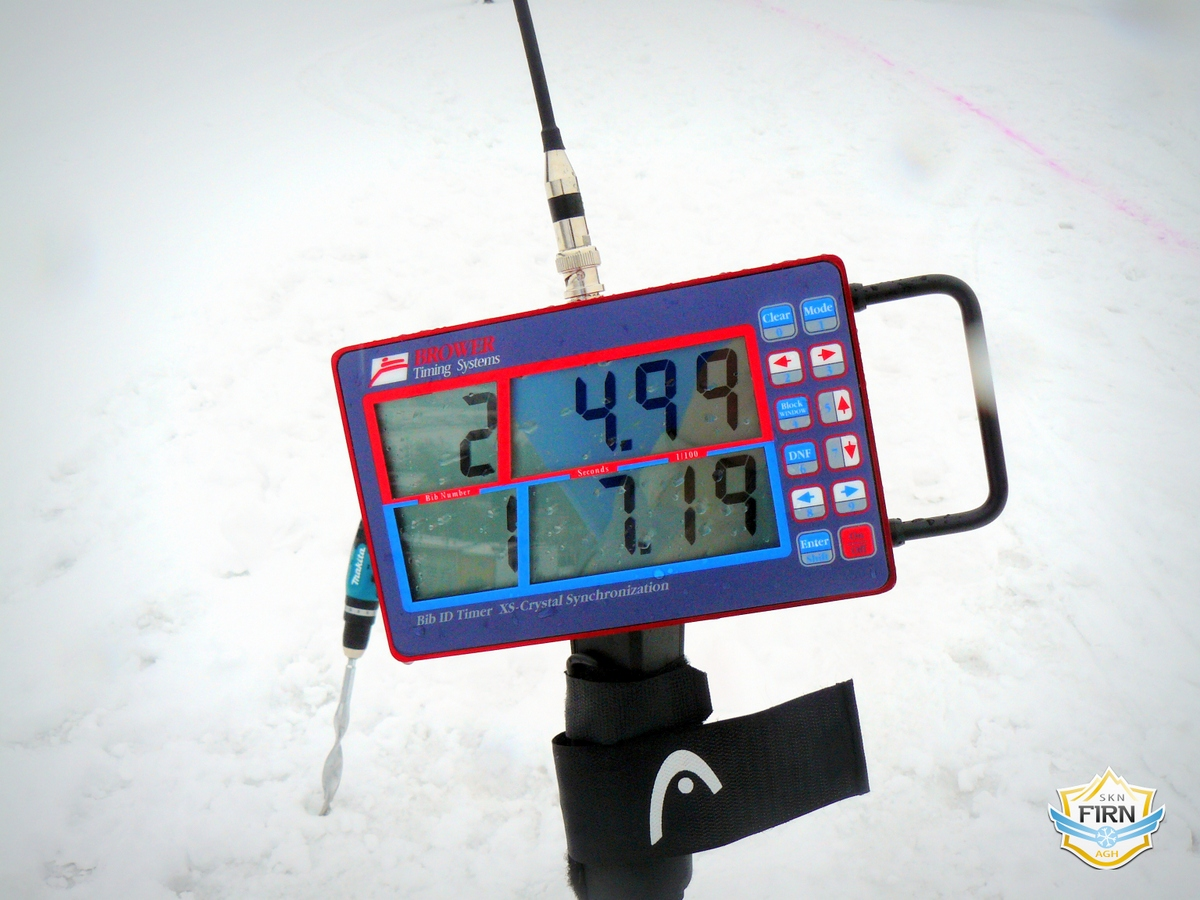
\includegraphics[height=220px]{eksp-3}
\caption{Zegar marki \textit{Brower}, u�yty do przeprowadzenia eksperymentu. Sprz�t u�yczony dzi�ki �yczliwo�ci Studenckiego Klubu Narciarskiego FIRN AGH}
\label{fig:eksp-3}
\end{figure}

Zmierzone czasu by�y istotnie r�ne: 6.48 s dla narciarza na bardzo dobrze przygotowanych nartach i 7.19 s dla bardzo s�abo przygotowanych nart. Nale�y zwr�ci� uwag�, �e jest to r�nica o ponad 0.7 s i to wypracowana na bardzo kr�tkim odcinku. Czas przejazdu na �le przygotowanych nartach jest o ponad 10\% d�u�szy. Zazwyczaj przejazd zawodnika na trasie zawod�w narciarskich trwa mi�dzy 30 a 120 s, wi�c r�nica b�dzie si� znacz�co pog��bia�. Zosta�o zatem potwierdzone eksperymentalnie, �e warto dba� o �lizgi narty, nie tylko dla zwi�kszenia komfortu jazdy i lepszej konserwacji sprz�tu, ale r�wnie� dla osi�gania lepszych wynik�w w zawodach.

Kolejny eksperyment mia� na celu zbadanie jak wp�ynie na czas przejazdu poruszanie si� po �wie�ym �niegu, zamiast po wy�lizganym ju� torze. Jako sta�y warunek eksperymentu dodajemy zatem u�yte narty - w tym przypadku dobrze przygotowane. W tym eksperymencie narciarz ubrany by� w gum� narciarsk� i porusza� si� za ka�dym razem w pozycji obni�onej tzn. ,,\textit{na jajo}''. Zmieniany by� natomiast tor przejazdu:
\begin{itemize}
\item wy�lizgany tor,
\item cienka warstwa �wie�ego �niegu.
\end{itemize}

Zmierzone czasy by�y ponownie istotnie r�ne. Przejazd po wy�lizganym torze zaj�� 5.98 s, natomiast po dziewiczym torze a� 7.19 s. Jest to ponownie, gigantyczna r�nica w uj�ciu tak kr�tkiego czasu przejazdu - czas po dziewiczym �niegu jest o ponad 22\% gorszy. 

Podsumowuj�c eksperymenty dynamiczne: zar�wno rodzaj pod�o�a, jak i stan �lizgu narty wp�ywaj� w bardzo znacz�cy spos�b na warto�� wsp�czynnika tarcia, a w konsekwencji na czas pokonywania trasy.

\subsection{Si�a oporu powietrza}
\label{silaOporuEksperymnet}

\paragraph{Za�o�enia i warunki eksperymentu} 
Kolejny eksperyment przeprowadzany by� ju� tylko na stoku narciarskim - Siepraw Ski w pobli�u Krakowa. Eksperyment mia� na celu sprawdzenie zale�no�ci pomi�dzy powierzchni� narciarza a czasem jego przejazdu. Poniewa� za zmienn� eksperymentu przyjmujemy tylko powierzchni� narciarza, sprawdzamy tak naprawd� zale�no�� pomi�dzy powierzchni� a warto�ci� si� oporu powietrza. Przygotowane zosta�y nast�puj�ce scenariusze:
\begin{itemize}
\item narciarz ubrany jest w tzw. \textit{gum� narciarsk� }przylegaj�c� do cia�a. Str�j ten opisany jest szerzej w sekcji \ref{sec:oporPowietrza} na stronie \pageref{sec:oporPowietrza}. Narciarza w tym stroju mo�na zobaczy� na rysunku \ref{fig:eksp-4} na stronie \pageref{fig:eksp-4}.  Narciarz przyjmuje dwa warianty pozycji:
\begin{itemize}
\item pozycj� podwy�szon�, 
\item pozycj� na tzw. jajo (widoczn� na rysunku \ref{fig:eksp-4}).
\end{itemize}
\item narciarz ubrany jest w klasyczny str�j narciarski, czyli spodnie narciarskie i kurtk�. Narciarz przyjmuje pozycj� podwy�szon� - zobrazowane to jest na rysunku \ref{fig:eksp-5} na stronie \pageref{fig:eksp-5}
\end{itemize}

Dodatkowo podczas eksperymentu panuj� nast�puj�ce sta�e warunki:
\begin{itemize}
\item kolorowym sprayem wyznaczono lini� wzd�u� linii spadku stoku o d�ugo�ci 28 metr�w, 
\item stok jest o sta�ym nachyleniu oko�o 8 stopni,
\item narciarz rozpoczyna przejazd bez odpychania si� kijami,
\item narciarz porusza si� po wyje�d�onym torze (brak �wie�ego �niegu),
\item bezwietrzna pogoda, warunki atmosferyczne nie zmieniaj� si� podczas trwania eksperymentu,
\item narciarz korzysta za ka�dym razem z tego samego sprz�tu narciarskiego.
\end{itemize}

\paragraph{Przebieg eksperymentu dla ka�dego wariantu pozycji}
\begin{itemize}
\item narciarz przyjmuje odpowiedni� pozycj� i rozpoczyna jazd�, co powoduje samoczynne uruchomienie zegara,
\item narciarz nie wykonuje �adnych ruch�w, stara si� tylko prowadzi� narty wzd�u� wyznaczonej linii,
\item narciarz przekracza lini� mety, co powoduje automatyczne zatrzymanie zegara,
\item czas przejazdu jest notowany.
\end{itemize}

\paragraph{Wyniki i Wnioski}

W pozycji podwy�szonej, ubrany w klasyczny str�j narciarski narciarz potrzebowa� 6.48 s na przebycie wyznaczonego odcinka (rysunek \ref{fig:eksp-5}). Zmiana stroju na bardziej op�ywowy - tj. ubranie tylko gumy narciarskiej, pozwoli�a zredukowa� czas przejazdu o 6.7\% - do 6.04 s. Jest to bardzo du�a r�nica na tak niewielkim odcinku. Kolejna optymalizacja, czyli przyj�cie pozycji zjazdowej tzw. na jajo (widocznej na rysunku \ref{fig:eksp-4}), pozwoli�a zredukowa� czas przejazdu o kolejny 1\% uzyskuj�c czas 5.98 s.

Uda�o si� do�wiadczalnie pokaza�, �e zmiana powierzchni narciarza ma istotny wp�yw na czas przejazdu. Warunki prowadzenia eksperymentu i posiadany sprz�t nie pozwoli�y wyizolowa� zmian wielko�ci powierzchni narciarza, od zmian wsp�czynnika \textit{C}, z r�wnania na warto�� si�y oporu powietrza ze wst�pu teoretycznego ze strony \pageref{sec:oporPowietrza}. Nale�y bowiem zwr�ci� uwag�, �e guma narciarska nie tylko zmniejsza powierzchni� narciarza, ale znacz�co zwi�ksza jego ,,op�ywowo��'', a wi�c zmniejsza wsp�czynnik \textit{C}.

\begin{figure}[H]
\centering
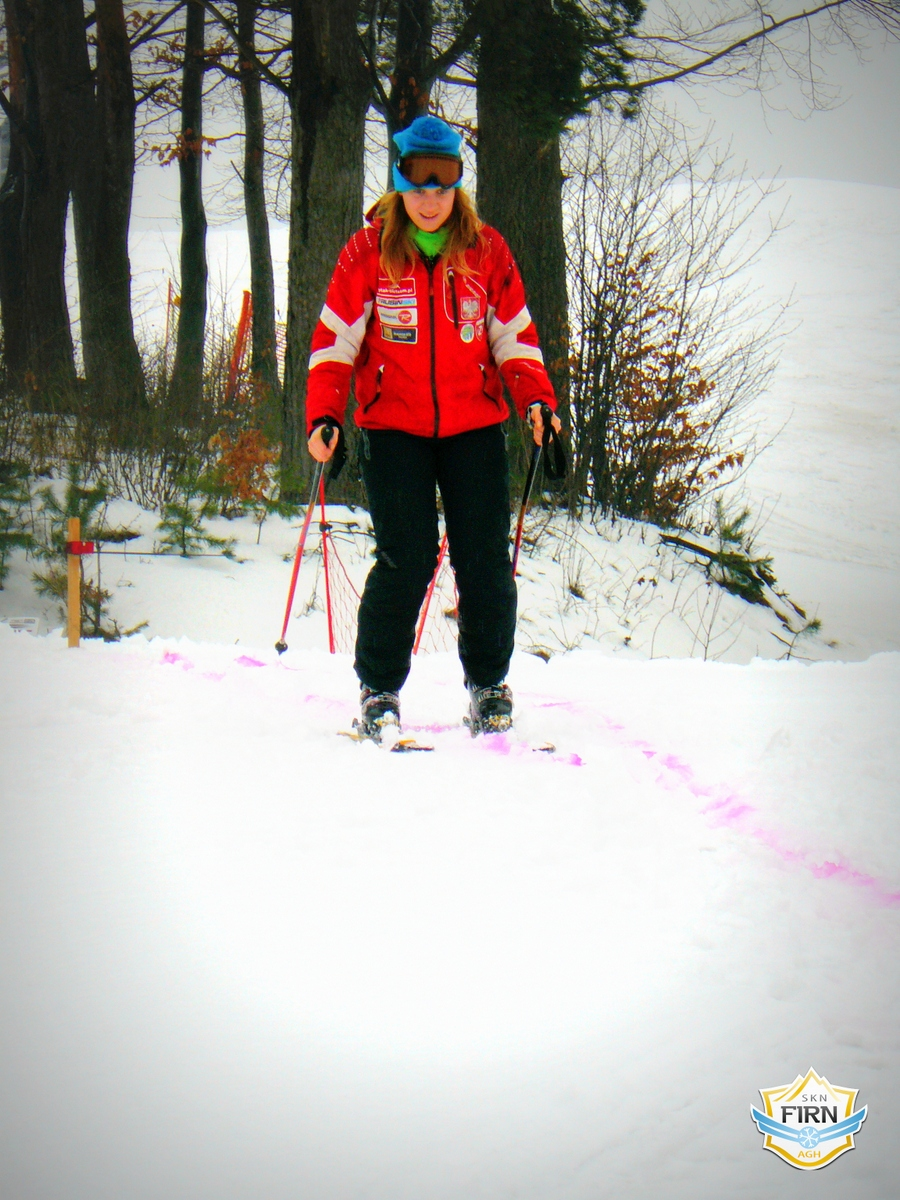
\includegraphics[height=220px]{eksp-5}
\caption{Narciarz w pozycji podwy�szonej, ubrany w klasyczny str�j narciarski sk�adaj�cy si� z kurtki narciarskiej i spodni narciarskich}
\label{fig:eksp-5}
\end{figure}

\begin{figure}[H]
\centering
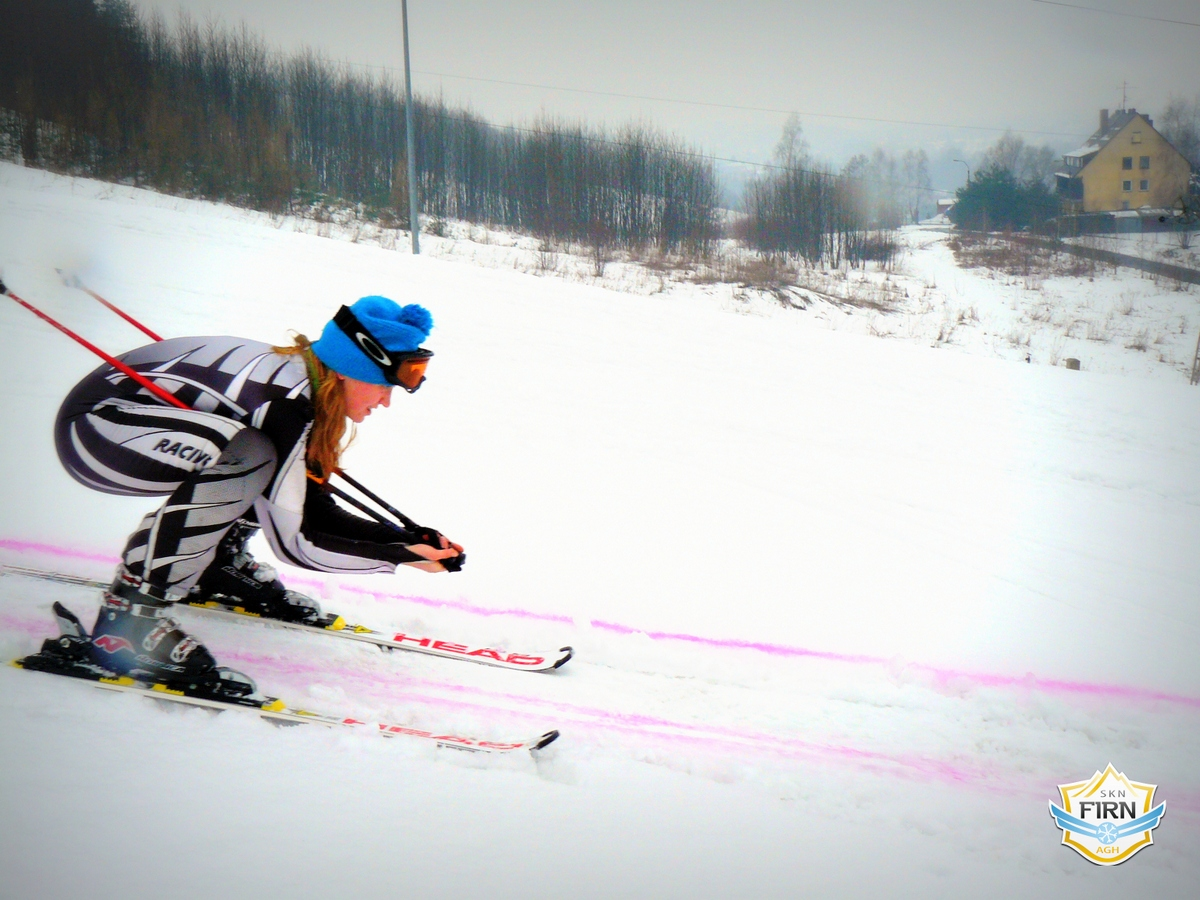
\includegraphics[height=220px]{eksp-4}
\caption{Narciarz w pozycji zjazdowej, ubrany w tzw. gum� narciarsk�}
\label{fig:eksp-4}
\end{figure}

\section{Jazda po �uku, a jazda w skos stoku}
\label{sec:jazda-po-luku}

Nawi�zuj�c do eksperymentu przeprowadzonego z u�yciem stworzonego przez nas modelu komputerowego, z sekcji \ref{sec:torJazdy} ze strony \pageref{sec:torJazdy}, kt�ry wykaza�, �e najbardziej optymalny pod wzgl�dem czasowym tor przejazdu z punktu A do B, wcale nie jest lini� prost� mi�dzy tymi punktami, a raczej fragmentem cykloidy, zaprojektowany zosta� analogiczny eksperyment na stoku narciarskim. Warunki wykonania eksperymentu nie s� idealne, aczkolwiek wystarczaj�ce, by zauwa�y� zak�adan� zale�no��.

\paragraph{Opis eksperymentu}
Na stoku oznaczony zosta� punkt startowy (A) oraz linia mety z oznaczonym �rodkiem mety (B). Nast�pnie na �niegu zosta�a oznaczona sprayem linia prosta mi�dzy punktami startu a �rodkiem mety. Stok mia� sta�e, niewielkie nachylenie. Narciarz mia� za zadanie na jak najbardziej p�asko prowadzonych nartach pokona� zaznaczony odcinek z A do B. Zosta� zanotowany czas z kilku pr�b, a nast�pnie obliczona zosta�a �rednia: 6.12 s. Kolejnym zadaniem narciarza by�o przejechanie po p�ynnym �uku - z punktu A do B. Po kilku pr�bach doboru odpowiedniego promienia skr�tu uda�o si� przeprowadzi� kilka pr�b zako�czonych znalezieniem si� w punkcie B. Tor przejazdu po �uku zosta� oznaczony sprayem dla lepszego zobrazowania eksperymentu. Czasy przejazdu z tych pr�b zosta�y zanotowane i r�wnie� obliczona zosta�a �rednia - wynosz�ca 5.49 s. Czas przejazdu istotnie r�ni si� zatem w zale�no�ci od toru. Oczywi�cie w gr� wchodzi tu ogromna liczba czynnik�w mi�dzy innymi inne tarcie pomi�dzy kraw�dziami narty a �niegiem, ni� w przypadku tarcia �lizgu narty o �nieg. Niezaprzeczalny jest jednak fakt, �e czas przejazdu by� o ponad 11\% d�u�szy dla jazdy w linii prostej w stosunku do jazdy po �uku. Warunki przeprowadzania eksperymentu s� dobrze widoczne na rysunku \ref{fig:eksp-6} na stronie \pageref{fig:eksp-6}.

\begin{figure}[H]
\centering
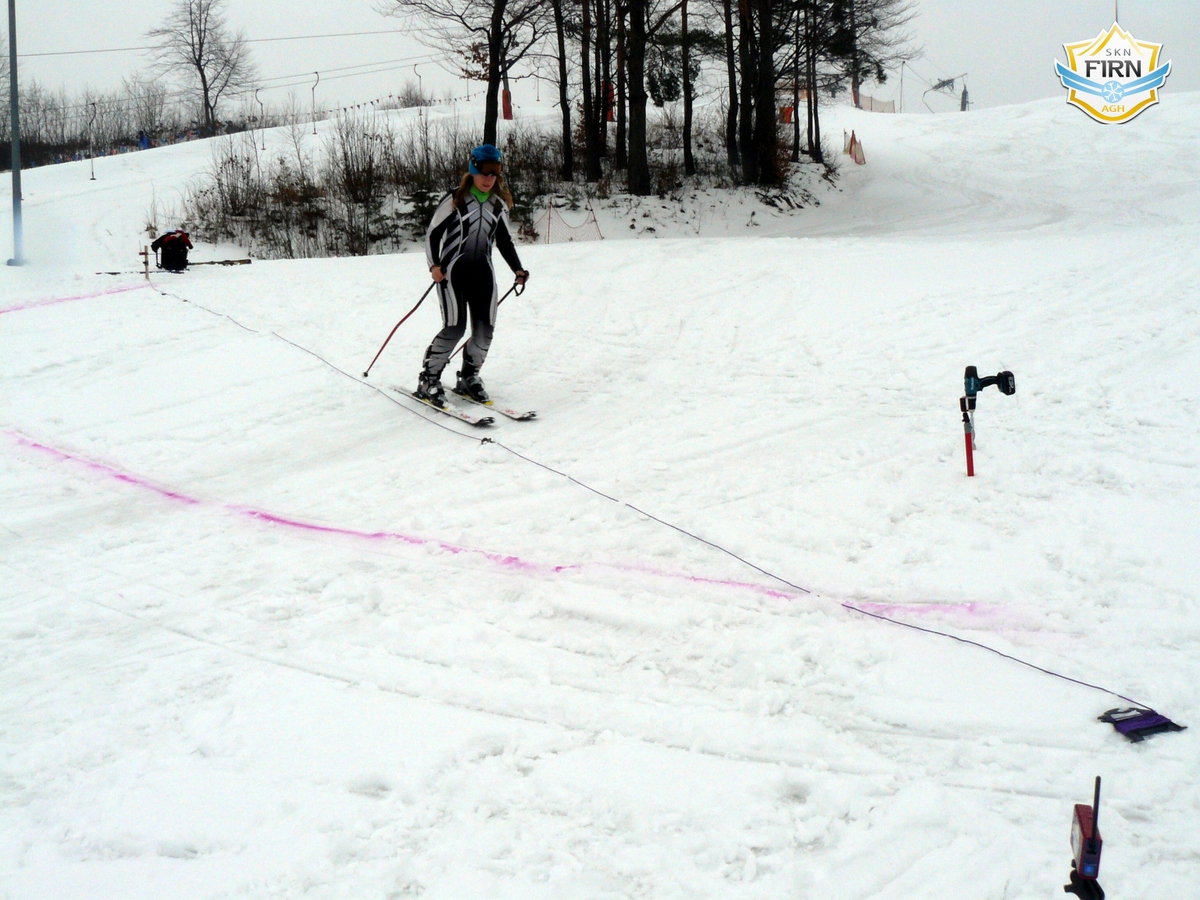
\includegraphics[height=220px]{eksp-6}
\caption{Eksperyment por�wnuj�cy przejazd pomi�dzy punktami, wybieraj�c jazd� po wycinku �uku, a jazd� w skos stoku na p�askich nartach} 
\label{fig:eksp-6}
\end{figure} 

\section{Optymalizacja}
\label{sec:optWyniki}

W tej cz�ci zostan� pokazane wyniki jakie zosta�y otrzymane jako efekt dzia�ania algorytmu ewolucyjnego w celu znalezienia optymalnej trasy przejazdu. Sprawdzimy, jak poszczeg�lne parametry algorytmu wp�ywaj� na czas jego dzia�ania oraz uzyskiwane wyniki. Spr�bujemy tak�e rozwi�za� problem dla trudniejszych przypadk�w: zwi�kszaj�c liczb� punkt�w, kt�re stanowi� rozwi�zanie oraz optymalizuj�c tras� d�u�szego slalomu. Nast�pnie zobaczymy, jak optymalizacja lokalna przyspieszy wykonanie programu.

\subsection{Algorytm ewolucyjny}
\label{sec:ewolucyjnyWyniki}
Wiedz�c, �e za�o�enia dotycz�ce modelu oraz spos�b poruszania si� narciarza mo�na uzna� za poprawne i zbli�one do tego co rzeczywi�cie dzieje si� podczas jazdy na stoku, przetestujemy teraz, jak sprawdza si� algorytm ewolucyjny do cel�w optymalizacji trasy slalomu.

W poni�szych eksperymentach wykorzystane zostanie nast�puj�ce ustawienie bramek: (5,13), (0,26), (5,39), (4,44), (11,57), (0,70). Ustawienie to jest podobne do tych, kt�re s� wybierane w rzeczywisto�ci. Posiada tak�e wertikal, figur� slalomow�, szerzej opisan� w sekcji \ref{sec:alpineSkiing}, cz�sto stosowan� w slalomie, kt�ra ma wymusza� zmian� rytmu, a wi�c b�dzie dobrym sprawdzianem dla zastosowanego algorytmu.

Zak�adamy, �e narciarz startuj�c ma pr�dko�� pocz�tkow� $1\frac{m}{s}$. Wynika to z tego, �e przy starcie zawodnicy zaczynaj� od odepchni�cia si� kijami od �niegu nadaj�c sobie pr�dko�� pocz�tkow�. Najwa�niejsze jest to, �e warto�� ta b�dzie sta�a dla wszystkich eksperyment�w.

W eksperymencie \ref{sec:lamana} zosta�o stwierdzone, �e odleg�o�ci w pionie pomi�dzy kolejnymi punktami wyznaczaj�cymi tras� powinna wynosi� 2-4 m. Zatem przyjmijmy, �e b�d� to 3 m, co dla wy�ej podanego slalomu daje nam nieca�e 30 punkt�w do optymalizacji.

Warto�ci parametr�w algorytmu ewolucyjnego s� takie, jak wymienione wcze�niej w rozdziale \ref{sec:ewolucyjnyRozw}. Korzystamy z algorytmu $(\mu + \lambda)$, gdzie $\mu = 30$, a $\lambda = 100$. W ka�dej iteracji najpierw krzy�ujemy osobniki z populacji tymczasowej, losuj�c pary rodzicielskie, a w wyniku krzy�owania powstaje zn�w 100 osobnik�w. Nast�pnie mutacji podlegaj� wszystkie z tych osobnik�w. Jedynym dodatkowym za�o�eniem jest nie zmienianie pozycji punkt�w przejazdu przez bramki - chcemy, aby narciarz przejecha� zawsze jak najbli�ej bramki. Je�li kt�ra� z warto�ci lub zastosowanych algorytm�w zmienia si�, jest to zaznaczone w eksperymencie.


\subsubsection{Warunek zako�czenia}
Warunkiem stopu w zastosowanym algorytmie ewolucyjnym jest sprawdzenie, czy populacja, na kt�rej dzia�amy przesta�a by� ju� zr�nicowana. Dodatkowo, je�li r�nica pomi�dzy najlepszym a najgorszym osobnikiem jest ma�a, czekamy przez okre�lon� liczb� iteracji, aby sprawdzi�, czy uzyskujemy jeszcze jak�� popraw� najlepszego osobnika, ale wi�ksz� ni� zadana granica. Je�li taka sytuacja nie zachodzi, oznacza to, �e szanse na popraw� wyniku s� niewielkie i mo�na zako�czy� dzia�anie algorytmu. W rozwi�zaniu tym istniej� jednak trzy parametry, kt�rych wp�yw na ostateczny wynik zbadamy w tym eksperymencie. 

\paragraph{Eksperyment 1.} W pierwszym eksperymencie parametry zako�czenia algorytmu wynosz�:
\begin{itemize}
\item dla zr�nicowania populacji przyjmujemy na pocz�tek warto�� 0.1, czyli 10\%, gdzie warto�� ta obliczana jest na podstawie najlepszej i najgorszej warto�ci fitness w populacji, poprzez znalezienie r�nicy tych warto�ci i podzielenie otrzymanej warto�ci przez warto�� najlepsz� (aby uzyska� warto�� w \% mno�ymy przez 100\%),
\item zmiana najlepszego osobnika jest uznawana za wystarczaj�co du��, je�li wyniesie przynajmniej 0.3 s,
\item liczba iteracji przez kt�re czekamy na zmian� najlepszego osobnika, to na pocz�tek 7.
\end{itemize}

W zwi�zku z tym, �e zachowanie algorytmu jest niedeterministyczne, dla ka�dego zestawu parametr�w zosta�y przeprowadzone po trzy eksperymenty, aby mo�na by�o u�redni� wyniki i por�wna� eksperymenty mi�dzy sob�.

Poni�ej (rysunki \ref{fig:w1s} oraz \ref{fig:w1w}) znajduj� si� wyniki wizualne przeprowadzonego eksperymentu. Na kolejnych obrazkach widoczne s� odpowiednio wszystkie trzy znalezione najlepsze trasy oraz wykresy zmian warto�ci fitness odpowiednio: najlepszego osobnika w ka�dej iteracji (kolor czerwony), najgorszego osobnika (kolor zielony) oraz �rednia warto�� fitness ca�ej populacji (kolor niebieski). Kolejno�� slalom�w odpowiada kolejno�ci wykres�w.

\newpage
\begin{figure}[H]
\centering
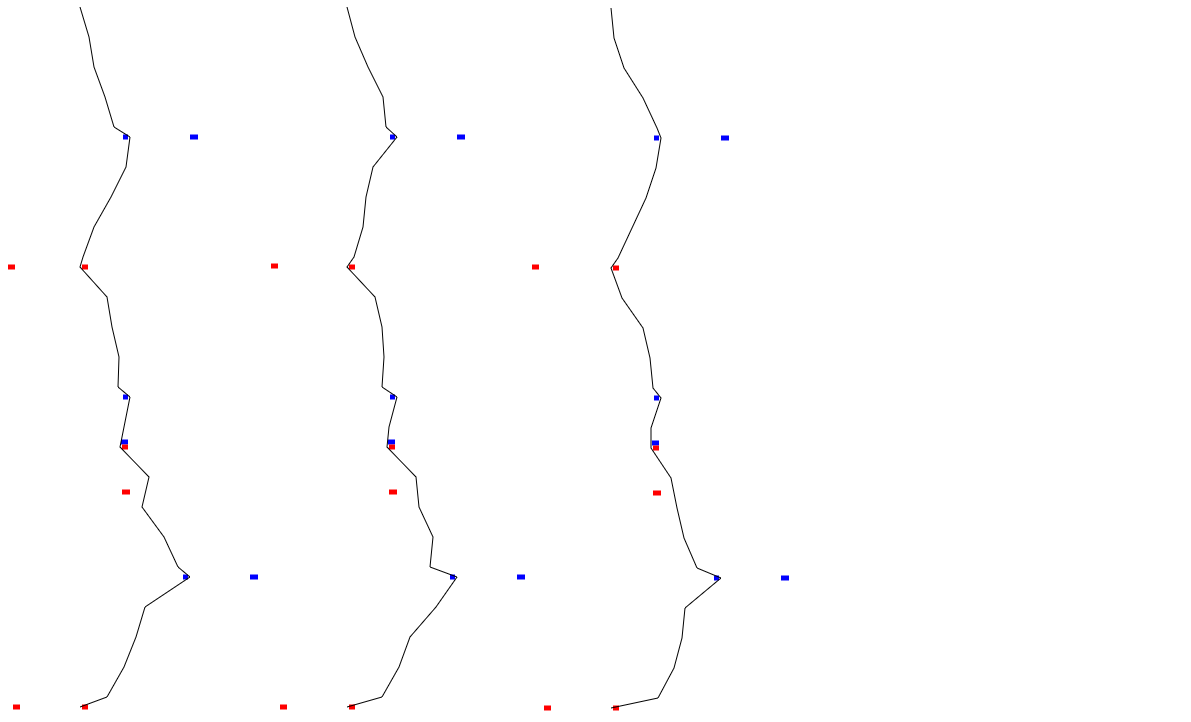
\includegraphics[scale=0.8]{wyniki/wynik1-s}
\caption{Wyniki z kolejnych pr�b dla parametr�w zako�czenia: 10\%, 0.3 s i 7}
\label{fig:w1s}
\end{figure}

\begin{figure}[h]
\centering
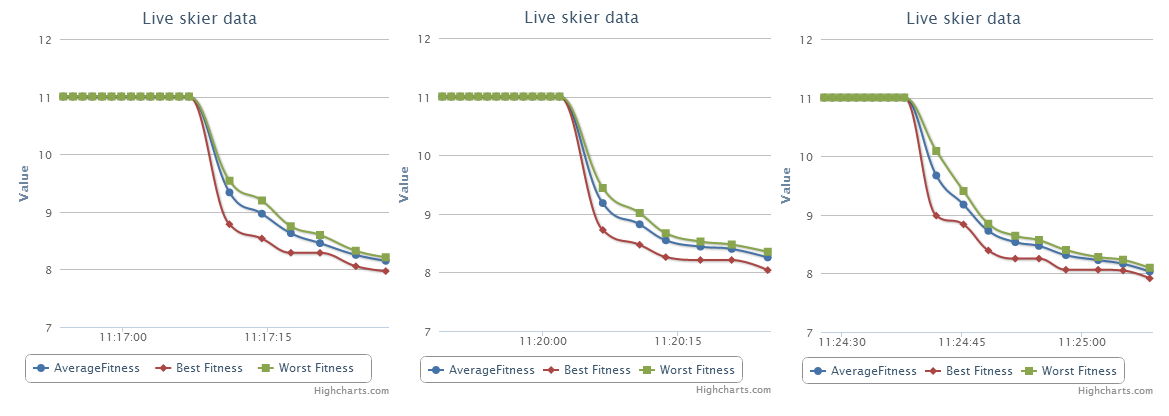
\includegraphics[scale=0.5]{wyniki/wynik1-w}
\caption{Wykresy z kolejnych pr�b dla parametr�w zako�czenia: 10\%, 0.3 s i 7}
\label{fig:w1w}
\end{figure}

\newpage
Oto otrzymane czasy przejazdu dla kolejnych pr�b:

\begin{table}[H]
\caption{Czasy przejazdu dla kolejnych pr�b wraz z liczb� iteracji oraz czasem dzia�ania algorytmu}
\centering
\begin{tabular}{ | c | c | c | c |}
  \hline                        
  numer pr�by & czas przejazdu [s] & liczba iteracji & czas dzia�ania [s] \\ \hline  
1 & 7.968 & 7 & 18 \\ \hline
2 & 8.039 & 7 & 19 \\ \hline
3 & 7.917 & 9 & 21 \\ \hline
\end{tabular}
\end{table}

Zatem �redni czas przejazdu w tych trzech pr�bach wyni�s� 7.975 s.

Liczba iteracji w przypadku tych wynik�w wynios�a 7-9. Algorytm bardzo szybko dochodzi� do rozwi�zania, a czas dzia�ania to tylko ok. 20 s. Trzeba jednak pami�ta�, �e czas dzia�ania algorytmu musi by� wystarczaj�co du�y, aby mia�o sens przesy�anie problemu z serwera - najlepiej oko�o kilku minut. Wtedy czas oblicze� b�dzie znacz�co d�u�szy w stosunku do czasu przesy�u danych.

Jednocze�nie, co obserwujemy na rysunkach, wyniki nie s� satysfakcjonuj�ce - trasa przejazdu nie jest g�adka i z pewno�ci� istnieje lepsze rozwi�zanie. Jednak skoro zosta�o wykonanych tylko kilka iteracji algorytmu, oznacza to, �e mo�na spr�bowa� uzyska� lepsze wyniki poprzez wyd�u�enie czasu dzia�ania algorytmu.

\paragraph{Eksperyment 2.} Wprowadzamy teraz zmian� w warto�ci parametru oznaczaj�cego r�nic� w fitness najlepszego osobnika. Zamiast warto�ci 0.3 s teraz b�dzie to 0.1 s. Sprawdzimy zar�wno, czy czas dzia�ania algorytmu si� wyd�u�y jak i czy uda si� przez to otrzyma� lepszy wynik.

Na rysunkach \ref{fig:w2s} oraz \ref{fig:w2w} a tak�e w tabeli \ref{tab:tab2} zebrane s� wyniki eksperymentu.

\begin{table}[H]
\caption{Czasy przejazdu dla kolejnych pr�b wraz z liczb� iteracji oraz czasem dzia�ania algorytmu}
\label{tab:tab2}
\centering
\begin{tabular}{ | c | c | c | c |}
  \hline                        
  numer pr�by & czas przejazdu [s] & liczba iteracji & czas dzia�ania [s] \\ \hline  
1 & 7.916 & 15 & 49 \\ \hline
2 & 7.809 & 14 & 46 \\ \hline
3 & 7.777 & 16 & 51 \\ \hline
\end{tabular}
\end{table}

�rednia uzyskanych czas�w przedstawionych w tabeli \ref{tab:tab2} wynosi: 7.834 s.

\newpage
\begin{figure}[H]
\centering
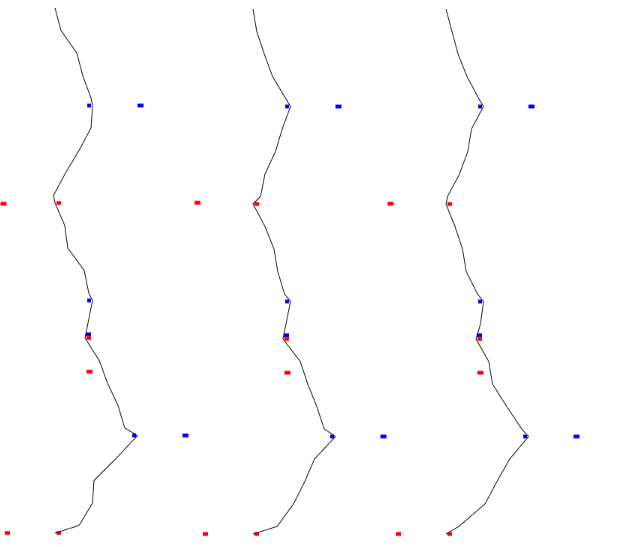
\includegraphics[scale=0.9]{wyniki/wynik2-s}
\caption{Wyniki z kolejnych pr�b dla parametr�w zako�czenia: 10\%, 0.1 s i 7}
\label{fig:w2s}
\end{figure}

\begin{figure}[H]
\centering
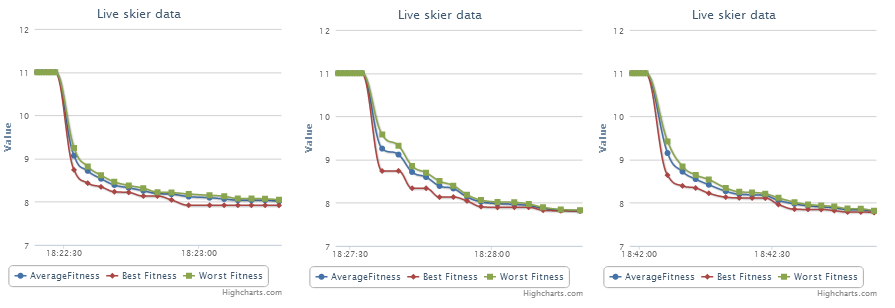
\includegraphics[scale=0.7]{wyniki/wynik2-w}
\caption{Wykresy z kolejnych pr�b dla parametr�w zako�czenia: 10\%, 0.1 s i 7}
\label{fig:w2w}
\end{figure}

\newpage
Wyniki poprawi�y si�, linia przejazdu jest du�o g�adsza, a czasy poprawi�y si� o ok. 0.15 s, czyli o ok. 2\%. Jednak czas dzia�ania algorytmu wyd�u�y� si� do 45-50 s, a liczba iteracji wynios�a 14-16. Oczywi�cie czas ten jest wci�� na tyle ma�y, �e mo�emy wprowadza� dalsze zmiany, kt�re wyd�u�� czas dzia�ania i jednocze�nie umo�liwi� znalezienie lepszego rozwi�zania.

\paragraph{Eksperyment 3.} Spr�bujmy w takim razie zmieni� r�wnie� parametr dotycz�cy zr�nicowania populacji - niech b�dzie to teraz nie 10\%, a 1\%.

Poni�ej znajduj� si� zebrane wyniki w tabeli \ref{tab:tab3} oraz na rysunkach \ref{fig:w3s} oraz \ref{fig:w3w}.

\begin{table}[H]
\caption{Czasy przejazdu dla kolejnych pr�b wraz z liczb� iteracji oraz czasem dzia�ania algorytmu}
\centering
\label{tab:tab3}
\begin{tabular}{ | c | c | c | c |}
  \hline                        
  numer pr�by & czas przejazdu [s] & liczba iteracji & czas dzia�ania [s] \\ \hline  
1 & 7.818 & 17 & 55 \\ \hline
2 & 7.822 & 14 & 45 \\ \hline
3 & 7.817 & 14 & 47 \\ \hline
\end{tabular}
\end{table}

�rednia zmierzonych wynik�w wynosi: 7.819 s.

\begin{figure}[H]
\centering
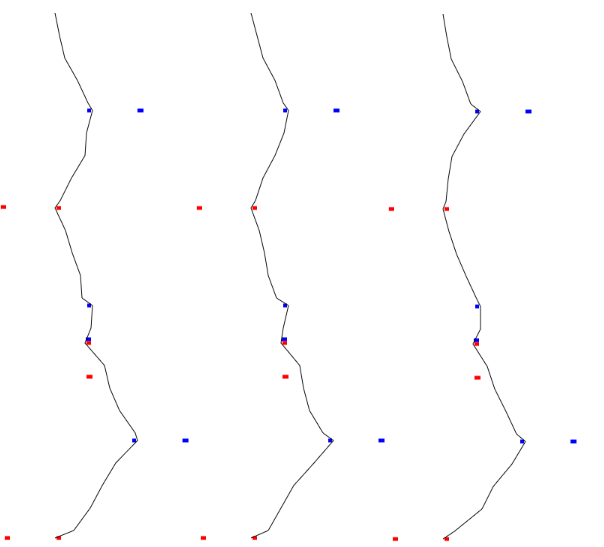
\includegraphics[scale=0.9]{wyniki/wynik3-s}
\caption{Wyniki dla kolejnych pr�b eksperymentu dla parametr�w zako�czenia: 1\%, 0.1 s i 7}
\label{fig:w3s}
\end{figure}

\begin{figure}[H]
\centering
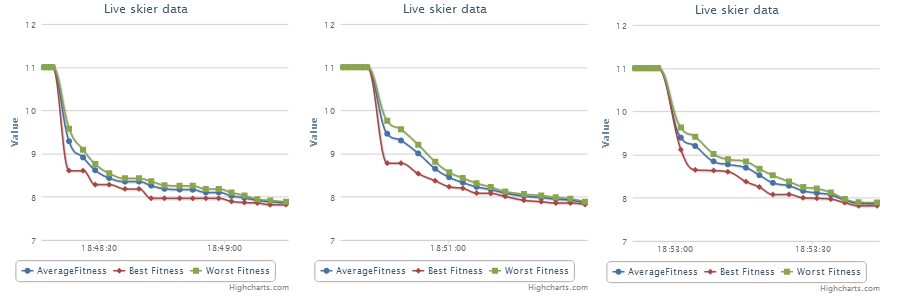
\includegraphics[scale=0.7]{wyniki/wynik3-w}
\caption{Wykresy dla kolejnych pr�b eksperymentu dla parametr�w zako�czenia: 1\%, 0.1 s i 7}
\label{fig:w3w}
\end{figure}

Jak wida� wyniki s� niewiele lepsze ni� te poprzednie. Zatem ten warunek praktycznie nie zmieni� zachowania. Pozosta� natomiast jeszcze warunek liczby iteracji, przez kt�re sprawdzamy, czy poprawia si� fitness najlepszego osobnika.

\paragraph{Eksperyment 4.} Zmieniamy teraz warto�� liczby iteracji, przez kt�re czekamy na zmian� najlepszego osobnika z 7 na 10.

\begin{table}[H]
\caption{Czasy przejazdu dla kolejnych pr�b wraz z liczb� iteracji oraz czasem dzia�ania algorytmu}
\centering
\label{tab:tab4}
\begin{tabular}{ | c | c | c | c |}
  \hline                        
  numer pr�by & czas przejazdu [s] & liczba iteracji & czas dzia�ania [s] \\ \hline  
1 & 7.892 & 13 & 41 \\ \hline
2 & 7.743 & 19 & 60 \\ \hline
3 & 7.837 & 13 & 41 \\ \hline
\end{tabular}
\end{table}

�rednia wynik�w wynosi: 7.824 s. Warto zwr�ci� uwag�, �e �rednio w ka�dym eksperymencie wykonywanych jest 1950 symulacji. Zale�y to od liczby osobnik�w w populacji oraz populacji tymczasowej, a wi�c parametr�w $\mu$ i $\lambda$, a tak�e od liczby iteracji wykonywanych w ka�dym eksperymencie.

\begin{figure}[H]
\centering
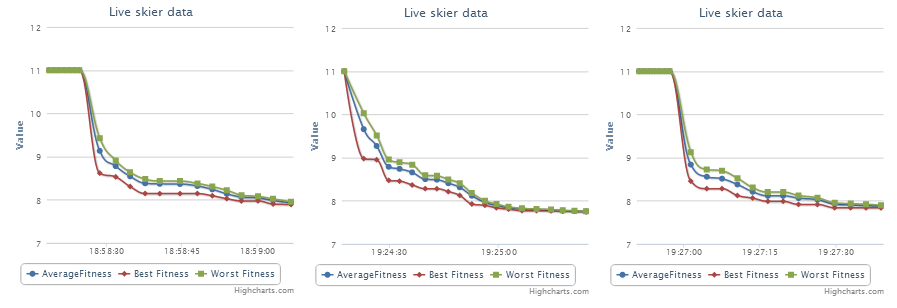
\includegraphics[scale=0.7]{wyniki/wynik4-w}
\caption{Wykresy dla kolejnych pr�b eksperymentu dla parametr�w zako�czenia: 1\%, 0.1 s i 10}
\label{fig:w4w}
\end{figure}

\newpage
\begin{figure}[H]
\centering
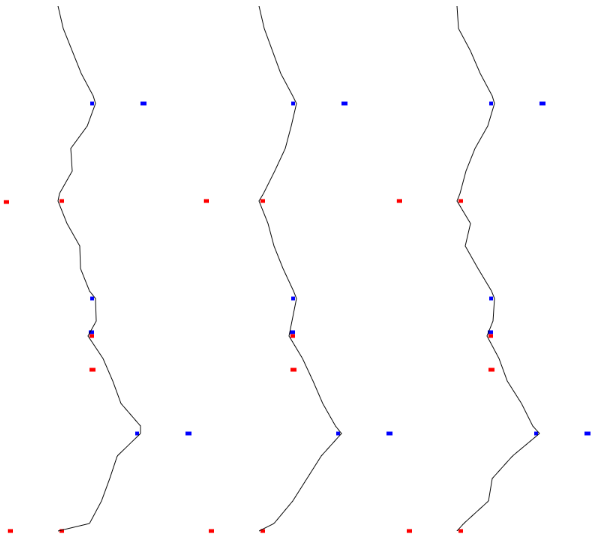
\includegraphics[scale=0.9]{wyniki/wynik4-s}
\caption{Wyniki dla kolejnych pr�b eksperymentu dla parametr�w zako�czenia: 1\%, 0.1 s i 10}
\label{fig:w4s}
\end{figure}

Jak wida�, r�wnie� zmiana tego parametru nie wnosi poprawy, cho� uda�o si� otrzyma� dotychczas najlepszy wynik - 7.743 s. Poniewa� algorytm ten jest niedeterministyczny, trudno oceni�, jakie warto�ci parametr�w s� optymalne. Oczywi�cie mo�na dalej zmniejsza� ich warto�ci w poszukiwaniu lepszego wyniku.

Warto jednak zauwa�y�, jaka jest charakterystyka trasy otrzymanej tu jako najlepsze rozwi�zanie (o numerze pr�by 2). Tor jazdy jest po prostu �aman�, kt�rej wierzcho�ki znajduj� si� w miejscach bramek - pomi�dzy kolejnymi bramkami linie s� w�a�ciwie odcinkami. Tym problemem zajmiemy si� w dalszej cz�ci, w rozdziale \ref{sec:wynikiStrategieKarania} opisuj�cym wyniki zastosowania funkcji kary.

W trakcie szczeg�owej analizy wynik�w z kolejnych iteracji (widocznych na wykresach), �atwo zauwa�y�, �e na pocz�tku poprawa wynik�w jest znacz�ca z ka�d� iteracj�, a pod koniec zmiany s� ju� niewielkie. Mo�na zatem pomy�le� o wprowadzeniu innego algorytmu, kiedy zmiany s� ju� s�abo widoczne, kt�ry skuteczniej znajdzie lepsze rozwi�zanie. Takim rozwi�zaniem jest na przyk�ad zastosowanie lokalnej optymalizacji. Wyniki tego podej�cia opisane s� w sekcji \ref{sec:lokalnaWyniki}.

Zanim przejdziemy jednak do wynik�w wprowadzenia lokalnej optymalizacji pozostaje jeszcze sprawdzi� ostatnie parametry algorytmu ewolucyjnego: $\mu$ i $\lambda$, a nast�pnie spr�bowa� rozwi�za� trudniejsze zadania, zwi�kszaj�c liczb� punkt�w stanowi�cych rozwi�zanie.

\subsubsection{Parametry $\mu$ i $\lambda$}
Do tej pory pocz�tkowa populacja liczy�a 30 osobnik�w, a populacja tymczasowa - 100. W literaturze najcz�ciej wymienia si� warto�ci oko�o 50 i 200 \cite{arabas}, warto zatem spr�bowa� zwi�kszy� te parametry, by sprawdzi� wi�cej przypadk�w rozwi�za�. Pozosta�e parametry pozostaj� jak w poprzednim eksperymencie.

\paragraph{Eksperyment 1.}
Sprawdzimy teraz jak wp�ywa na wyniki zmiana tych parametr�w, na pocz�tek spr�bujemy dla warto�ci odpowiednio 50 i 150.

\begin{figure}[H]
\centering
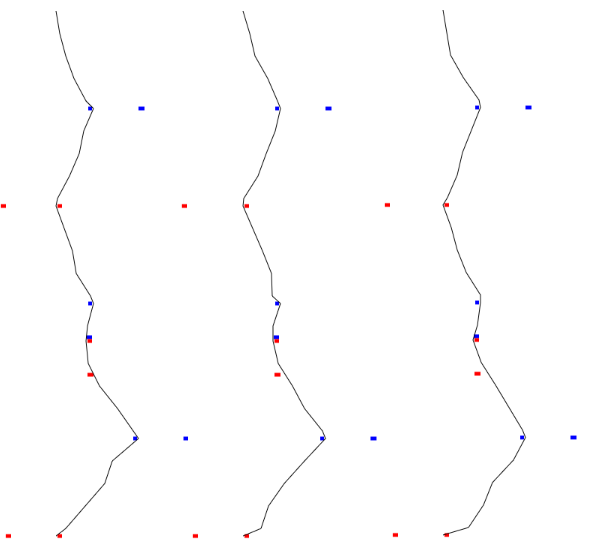
\includegraphics[scale=0.9]{wyniki/wynik5-s}
\caption{Wyniki dla kolejnych pr�b eksperymentu dla parametr�w $\mu=50$ i $\lambda=150$}
\label{fig:w5s}
\end{figure}

\begin{figure}[H]
\centering
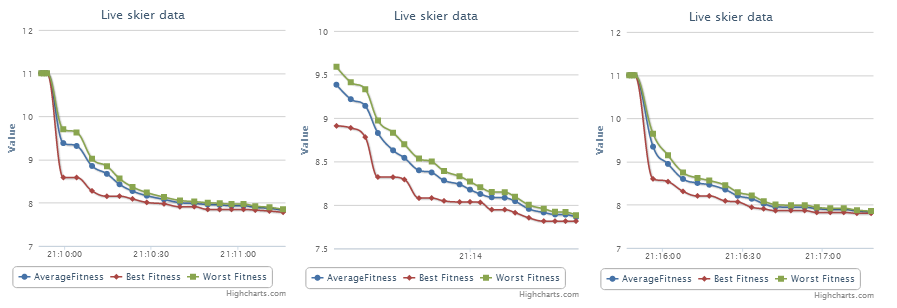
\includegraphics[scale=0.7]{wyniki/wynik5-w}
\caption{Wykresy dla kolejnych pr�b eksperymentu dla parametr�w $\mu=50$ i $\lambda=150$}
\label{fig:w5w}
\end{figure}

\begin{table}[h]
\caption{Czasy przejazdu dla kolejnych pr�b wraz z liczb� iteracji oraz czasem dzia�ania algorytmu ($\mu=50$ i $\lambda=150$)}
\centering
\label{tab:miLambda}
\begin{tabular}{ | c | c | c | c |}
  \hline                        
  numer pr�by & czas przejazdu [s] & liczba iteracji & czas dzia�ania [s] \\ \hline  
1 & 7.780 & 17 & 81 \\ \hline
2 & 7.814 & 21 & 109 \\ \hline
3 & 7.804 & 17 & 88 \\ \hline
\end{tabular}
\end{table}

�rednia wynik�w podanych w tabeli \ref{tab:miLambda} wynosi: 7.799 s. W tym przypadku �rednio w ka�dym eksperymencie zosta�o wykonanych oko�o 3670 symulacji.

Mo�na si� by�o spodziewa� poprawy wynik�w, jako, �e rozpatrujemy naraz wi�cej osobnik�w sprawdzaj�c wi�cej mo�liwych rozwi�za�, a wi�c zwi�kszaj�c prawdopodobie�stwo znalezienia lepszego rozwi�zania. Jednak poprawa jest niewielka, ale wa�ne jest to, �e do tej pory nie uda�o nam si� uzyska� tak dobrego �redniego wyniku. Pokazuje to, �e uda�o nam si� doprowadzi� do sytuacji, w kt�rej algorytm daje rzeczywi�cie cz�ciej lepsze wyniki, a uzyskane czasy s� zbli�one do siebie.
Takie wyniki zosta�y poniesione kosztem czasu wykonania algorytmu, kt�ry wzr�s� do ponad 80 s, a w jednym przypadku nawet 110 s.


\paragraph{Eksperyment 2.}
Zobaczmy jak zmieni� si� wyniki je�li warto�ci $\mu$ i $\lambda$ wynios� odpowiednio 60 i 200.

\begin{figure}[H]
\centering
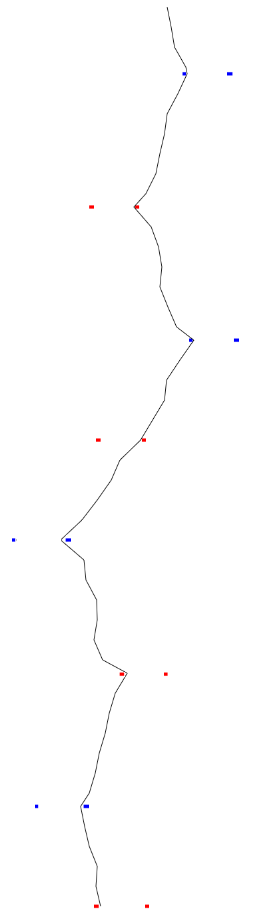
\includegraphics[scale=0.6]{wyniki/wynik6-s}
\caption{Wyniki dla kolejnych pr�b eksperymentu dla parametr�w $\mu=60$ i $\lambda=200$}
\label{fig:w6s}
\end{figure}

\begin{figure}[H]
\centering
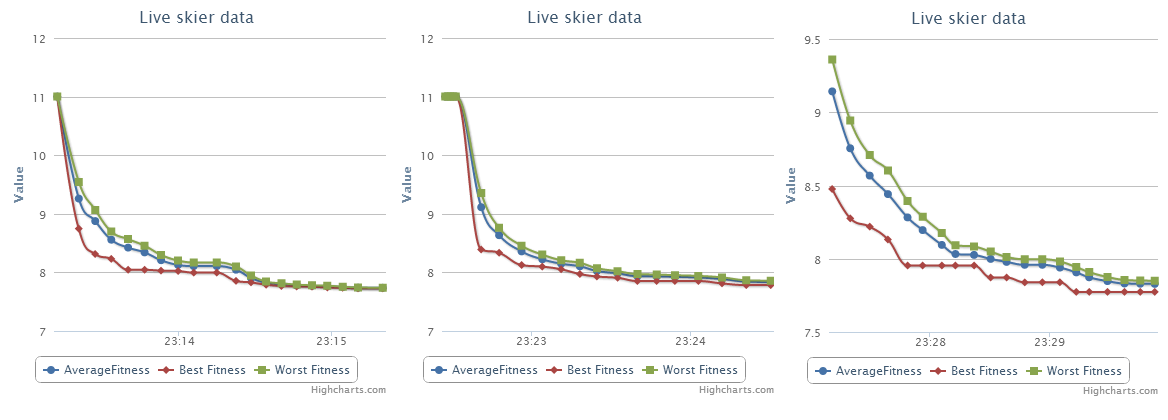
\includegraphics[scale=0.5]{wyniki/wynik6-w}
\caption{Wykresy dla kolejnych pr�b eksperymentu dla parametr�w $\mu=60$ i $\lambda=200$}
\label{fig:w6w}
\end{figure}

\begin{table}[h]
\caption{Czasy przejazdu dla kolejnych pr�b wraz z liczb� iteracji oraz czasem dzia�ania algorytmu ($\mu=60$ i $\lambda=200$)}
\centering
\begin{tabular}{ | c | c | c | c |}
  \hline                        
  numer pr�by & czas przejazdu [s] & liczba iteracji & czas dzia�ania [s] \\ \hline  
1 & 7.729 & 19 & 127 \\ \hline
2 & 7.783 & 15 & 118 \\ \hline
3 & 7.774 & 20 & 170 \\ \hline
\end{tabular}
\end{table}

�rednia wynik�w wynosi: 7.762 s. �rednio w ka�dym eksperymencie zosta�o wykonanych 4680 symulacji.

W tym przypadku wszystkie otrzymane czasy s� mniejsze ni� 7.8 s, a otrzymane linie przejazdu wygl�daj� bardzo dobrze. Warto r�wnie� zauwa�y�, �e w pierwszym przypadku otrzymali�my najlepszy czas - 7.729 s. Widzimy r�wnie�, �e zgodnie z oczekiwaniami, wyd�u�y� si� zn�w czas dzia�ania algorytmu. Minimalny czas to 118 s, czyli oko�o 2 minuty, a wykonanie trwa�o maksymalnie prawie 3 minuty. Takie czasy ju� mo�na uzna� za wystarczaj�ce, aby warto by�o rozsy�a� obliczenia, by by�y rozwi�zywane na innych w�z�ach obliczeniowych.

Dla por�wnania przeanalizujmy jak wp�yn�y zmiany parametr�w $\mu$ i $\lambda$ na uzyskiwane wyniki na podstawie zebranych wynik�w na wykresie \ref{fig:w6wyk}. Uwzgl�dniona jest tak�e �rednia liczba symulacji koniecznych do osi�gni�cia wyniku dla ka�dej pary ($\mu$ + $\lambda$).

\begin{figure}[h]
\centering
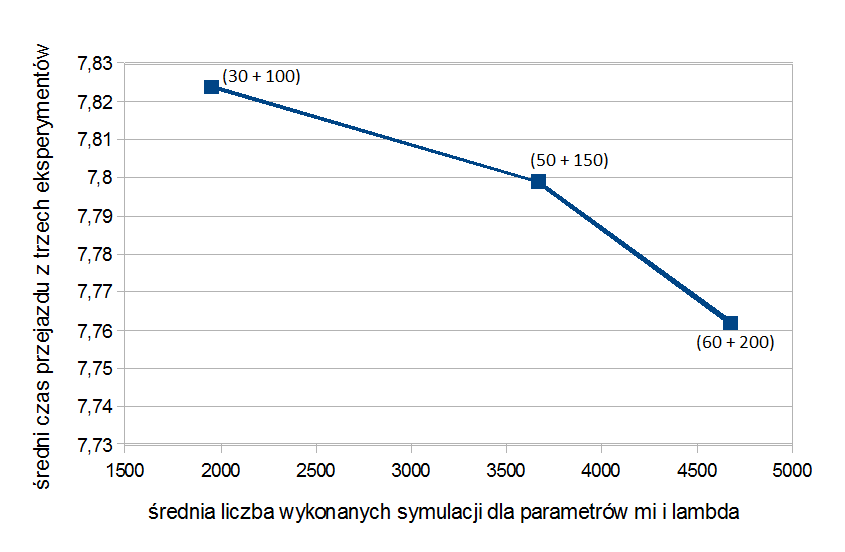
\includegraphics[scale=0.7]{wyniki/miLambda}
\caption{�redni czas przejazdu z wykonanych pr�b dla r�nych parametr�w $\mu$ i $\lambda$}
\label{fig:w6wyk}
\end{figure}

Wykres \ref{fig:w6wyk} pokazuje jak zmieni� si� �redni czas uzyskanych wynik�w odpowiednio dla kolejnych warto�ci parametr�w $\mu$ i $\lambda$. Wida�, �e cho� poprawa jest niewielka, bo o oko�o 0.05 s, to jednak widoczny jest trend wskazuj�cy, �e zwi�kszenie populacji wp�ywa pozytywnie na znajdowane rozwi�zanie. Poprawa jest lepsza w drugiej cz�ci wykresu, bior�c pod uwag� jak zmienia si� liczba symulacji koniecznych do osi�gni�cia wyniku w por�wnaniu z popraw� uzyskanego �redniego czasu przejazdu.

\subsubsection{G�sto�� siatki}
Aby uzyska� dok�adniejsze rozwi�zania mo�na spr�bowa� zag�ci� poziome linie wyznaczaj�ce ilo�� punkt�w stanowi�cych reprezentacj� trasy. Do tej pory linie te by�y w odleg�o�ci 3 m. Po zmianie na 2 m czas dzia�ania algorytmu powinien si� znacznie wyd�u�y� ze wzgl�du na wi�ksz� liczba rozpatrywanych punkt�w rozwi�zania. 

W eksperymencie warto�ci parametr�w wynosz� dla warunku zako�czenia: 
\begin{itemize}
\item dla zr�nicowania populacji przyjmujemy na warto�� 0.01, czyli 1\%,
\item zmiana najlepszego osobnika jest uznawana za wystarczaj�co du�� je�li wyniesie przynajmniej 0.05 s,
\item liczba iteracji, przez kt�re czekamy na zmian� najlepszego osobnika - 10.
\end{itemize}

Natomiast parametry $\mu$ i $\lambda$ przyjmijmy 30 i 100.

Na rysunkach \ref{fig:w7s} oraz \ref{fig:w7w} przedstawione s� wyniki z trzech przeprowadzonych pr�b.

\begin{figure}[H]
\centering
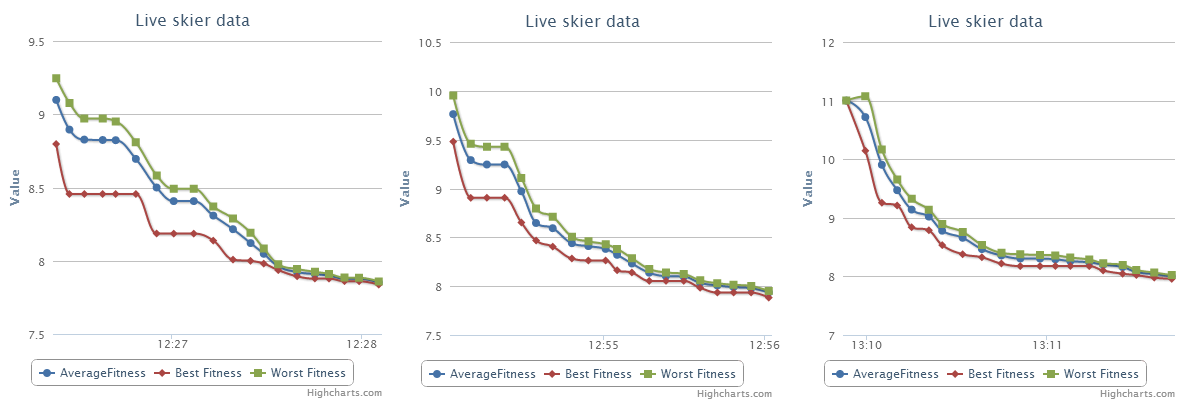
\includegraphics[scale=0.5]{wyniki/wynik7-w}
\caption{Wykresy dla kolejnych pr�b eksperymentu dla zwi�kszonej g�sto�ci siatki punkt�w rozwi�zania}
\label{fig:w7w}
\end{figure}

\begin{figure}[h]
\centering
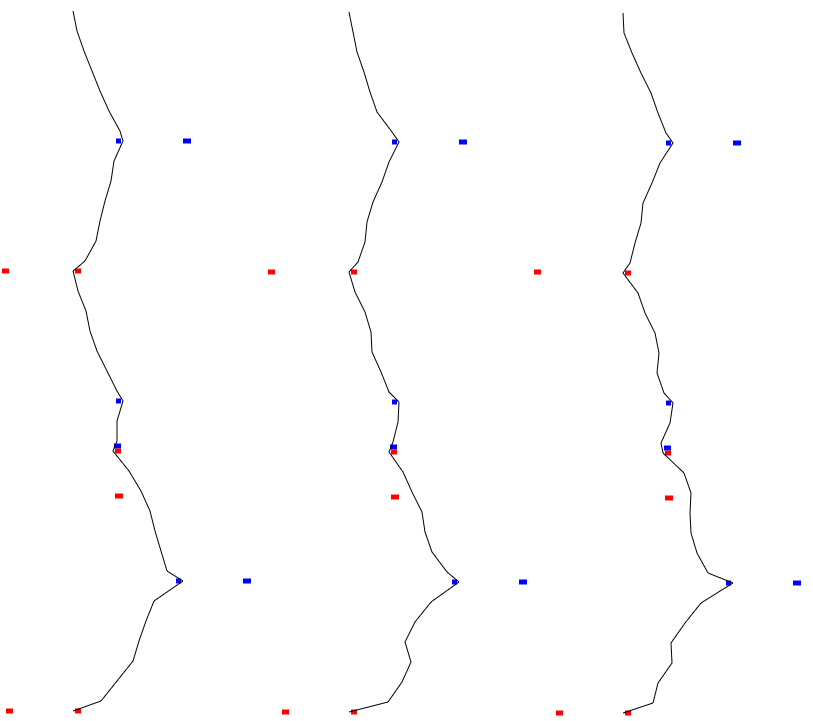
\includegraphics[scale=0.8]{wyniki/wynik7-s}
\caption{Wyniki dla kolejnych pr�b eksperymentu dla zwi�kszonej g�sto�ci siatki punkt�w rozwi�zania}
\label{fig:w7s}
\end{figure}

Czas wykonania wyd�u�y� si� do 100-150 s, a liczba iteracji zwi�kszy�a si� do ok. 20. Mimo zwi�kszenia dok�adno�ci, wci�� istniej� na trasie zbyt ostre zmiany kierunku, kt�re w rzeczywisto�ci s� niemo�liwe do wykonania bez dodatkowego czasu oraz zmniejszenia pr�dko�ci - obliczona trasa jest zbyt ``kanciasta''. Wydaje si�, �e taki spos�b optymalizacji nie umo�liwia nam znalezienia rzeczywi�cie najszybszej trasy. Zachodzi zatem konieczno�� wprowadzenia mechanizmu, kt�ry wyeliminuje zbyt ostre zmiany kierunku np. poprzez uwzgl�dnienie konieczno�ci zmniejszenia pr�dko�ci w miejscach o zbyt du�ym k�cie za�amania. Szczeg�owo, mechanizm ten opisany jest w sekcji \ref{sec:karanie} na stronie \pageref{sec:karanie}.

\subsubsection{D�uga trasa}
\label{dlugaTrasa}
Dotychczas rozpatrywany slalom by� jedynie fragmentem standardowego slalomu, czas przejazdu wynosi� mniej ni� 8 s. Pozostaje pytanie, czy dla wi�kszej liczby bramek algorytm nadal b�dzie w stanie znale�� rozwi�zanie zbli�one do optymalnego oraz jak du�o czasu b�dzie potrzebne do jego znalezienia. Mo�liwe te�, �e algorytm b�dzie potrzebowa� zmiany parametr�w, aby znale�� rozwi�zanie.

Sprawdzone zostanie teraz jakie wyniki otrzymamy dla d�u�szego slalomu: (19,10),(11,30),(20,50),(12,65), (0,80), (10,100), (3,120), (6,135)). Parametry $\mu$ i $\lambda$ pozostaj� ustawione na 30 i 100. Parametry zatrzymania algorytmu zostawiamy ustawione tak, aby algorytm dzia�a� d�u�ej:

\begin{itemize}
\item dla zr�nicowania populacji przyjmujemy na warto�� 0.01, czyli 1\%,
\item zmiana najlepszego osobnika jest uznawana za wystarczaj�co du�� je�li wyniesie przynajmniej 0.05 s,
\item liczba iteracji przez kt�re czekamy na zmian� najlepszego osobnika - 10.
\end{itemize}

Kolejne punkty rozwi�zania znajduj� si� w odleg�o�ci 3 m w pionie, co dla tej trasy daje 48 punkt�w do optymalizacji.

\begin{figure}[H]
\centering
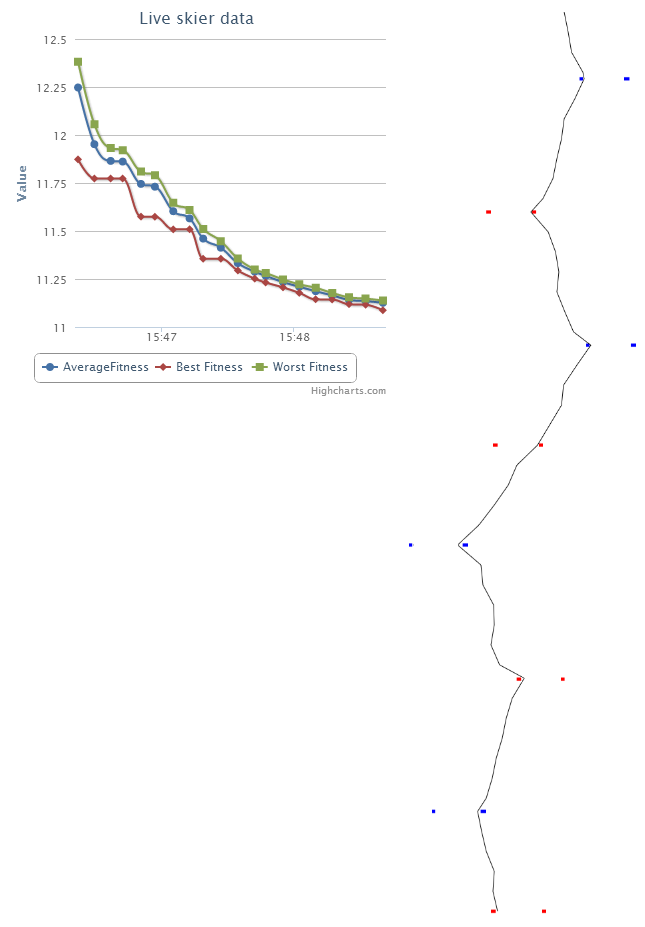
\includegraphics[scale=0.9]{wyniki/wynik8-ws}
\caption{Uzyskany wynik wraz z wykresem dla eksperymentu na d�u�szej trasie}
\label{fig:w8ws}
\end{figure}

Otrzymany wynik to 11.087 s. Obliczenia trwa�y 170 s, a algorytm potrzebowa� 23 iteracje do zako�czenia oblicze�. Zn�w mo�na powiedzie�, �e wynik jest dobry, jednak na pewno m�g�by by� lepszy - istnieje wiele ostrych zakr�t�w, zw�aszcza w okolicach bramek, rozwi�zanie nie jest idealne.

Warto zauwa�y�, �e wyd�u�enie trasy nie spowodowa�o natomiast wi�kszych problem�w je�li chodzi o znalezienie trasy, mimo zastosowanych warunk�w zako�czenia i zwi�kszenia liczby punkt�w z oko�o 30 na prawie 50.

\subsection{Lokalna optymalizacja}
\label{sec:lokalnaWyniki}
Algorytm ewolucyjny ma problem ze znalezieniem lepszych rozwi�za�, zw�aszcza kiedy dotychczas znalezione rozwi�zanie daje ju� dosy� dobry wynik, ale wci�� mo�na go�ym okiem zobaczy� miejsca, kt�re negatywnie wp�ywaj� na jako�� wyniku. Skoro algorytm nie radzi sobie b�d�c blisko rozwi�zania, mo�na spr�bowa� zastosowa� algorytm memetyczny - bazuj�c na rozwi�zaniu znalezionym przez algorytm ewolucyjny, dokonujemy dalszej optymalizacji wykorzystuj�c algorytm lokalnej optymalizacji. Mamy wtedy pewno��, �e znajdziemy rozwi�zanie nie gorsze od tego, na kt�rym bazujemy i dodatkowo, �e b�dzie ono najlepszym lokalnym rozwi�zaniem. Mo�emy mie� tak�e nadziej�, �e b�dzie to r�wnie� rozwi�zanie globalnie optymalne, ale pewno�ci takiej mie� nie mo�emy.

\paragraph{Eksperyment 1.}
Spr�bujmy zatem, bazuj�c na eksperymencie ``D�uga trasa'' w sekcji \ref{sec:ewolucyjnyWyniki} por�wna� jak poprawi si� otrzymany wynik dodaj�c na koniec oblicze� optymalizacj� lokaln� algorytmem Hill climbing. Wszystkie parametry oraz trasa przejazdu pozostaj� takie same jak w eksperymencie, do kt�rego si� odwo�ujemy.

\begin{figure}[h]
\centering
\includegraphics[scale=0.7]{wyniki/wynik9-wyk}
\caption{Wykres zmian czasu przejazdu w kolejnych iteracjach algorytmu HC}
\label{fig:w9wyk}
\end{figure}

\newpage
\begin{figure}[H]
\centering
\includegraphics[scale=0.9]{wyniki/wynik9-ws}
\caption{Por�wnanie wynik�w ES oraz HC wraz z wykresem dla eksperymentu na d�u�szej trasie}
\label{fig:w9ws}
\end{figure}

Na wykresie \ref{fig:w9ws} znajduje si� por�wnanie wyniku algorytmu ewolucyjnego oraz lokalnej optymalizacji. Czarna linia trasy jest rezultatem otrzymanym po dzia�aniu samego algorytmu ewolucyjnego, czas przejazdu po takiej trasie wynosi 11.06 s, a wi�c jest to czas zbli�ony do otrzymanego w eksperymencie bazowym. Algorytm ewolucyjny dzia�a� przez 21 iteracji.

Czerwona linia stanowi tras� uzyskan� po zastosowaniu algorytmu optymalizacji lokalnej na trasie znalezionej przez algorytm ewolucyjny. Na wykresie \ref{fig:w9wyk} mo�emy zobaczy� jak dok�adnie zmienia� si� czas przejazdu w ka�dej iteracji algorytmu lokalnego. Iteracja numer 0 to wynik otrzymany przez algorytm genetyczny. Po 7 iteracjach otrzymali�my wynik 10.825 s, co stanowi popraw� o 0.235 s, czyli ok. 2\%. Poprawa ta jest zdecydowanie zauwa�alna tak�e w kszta�cie slalomu i na pewno na tyle znacz�ca, �e decyduje o zwyci�stwie zawodnika.

\paragraph{Eksperyment 2.}
W eksperymencie pierwszym sprawdzili�my dzia�anie algorytmu lokalnego dla domy�lnie ustawionych parametr�w. W zastosowanym algorytmie Hill Climbing mamy mo�liwo�� zmiany dw�ch parametr�w:

\begin{itemize}
\item rozmiar kroku,
\item tzw. przyspieszenie (ang. \textit{acceleration}).
\end{itemize}

Szczeg�owy opis parametr�w mo�na znale�� w podrozdziale \ref{sec:hill}. W domy�lnym ustawieniu warto�ci tych parametr�w wynosz� odpowiednio 0.5 (odpowiadaj�ca 0.5 metra na rzeczywistej trasie) oraz 1.2 dla przyspieszenia. W przeprowadzonym eksperymencie poka�emy jak te parametry wp�ywaj� na ostateczne rozwi�zanie. Na tym samym rezultacie dzia�ania algorytmu genetycznego uruchomimy trzy razy algorytm lokalnej optymalizacji, ale z zestawami parametr�w przedstawionymi w tabeli \ref{tab:paramHill}.

Jak zostanie pokazane w nast�pnym eksperymencie, stosowanie mechanizmu karania poprawia otrzymywane wyniki, wi�c ten sam eksperyment wykonamy tak�e z zastosowaniem tego mechanizmu.

\begin{table}[h]
\caption{Warto�ci parametr�w algorytmu Hill climbing w kolejnych eksperymentach}
\centering
\label{tab:paramHill}
\begin{tabular}{ | c | c | c |}
  \hline                        
  nr pr�by & wielko�� kroku [m] & przyspieszenie \\ \hline  
  1 & 0.5 & 1.2 \\ \hline
  2 & 0.3 & 1.2 \\ \hline
  3 & 0.3 & 1.1 \\ \hline
\end{tabular}
\end{table}

\newpage
\begin{figure}[H]
\centering
\includegraphics[scale=0.8]{wyniki/wynik11-ws1}
\caption{Wyniki kolejnych pr�b eksperymentu z r�nymi warto�ciami parametr�w algorytmu HC}
\label{fig:w11ws}
\end{figure}

\begin{figure}[H]
\centering
\includegraphics[scale=0.8]{wyniki/wynik11-ws2}
\caption{Wyniki kolejnych pr�b eksperymentu z r�nymi warto�ciami parametr�w algorytmu HC z zastosowaniem PF}
\label{fig:w11ws2}
\end{figure}

Rysunki \ref{fig:w11ws} i \ref{fig:w11ws2} pokazuje otrzymane trasy dla r�nych algorytm�w i parametr�w:
\begin{itemize}
\item trasa czarna - trasa uzyskana w wyniki dzia�ania algorytmu ewolucyjnego,
\item trasa czerwona - optymalizacja lokalna z parametrami domy�lnymi,
\item trasa niebieska - optymalizacja lokalna z krokiem 0.3 m,
\item trasa zielona - optymalizacja lokalna z krokiem 0.3 m oraz przyspieszeniem 1.1.
\end{itemize}

Trasy otrzymane w wyniku dzia�ania algorytmu optymalizacji lokalnej r�ni� si� miejscami od siebie, cho� w niewielkim stopniu. Ma�e zr�nicowanie wynika z tego, �e pocz�tkowa trasa, kt�r� nale�a�o zoptymalizowa� by�a w ka�dym przypadku taka sama. Algorytm Hill Climbing jest algorytmem deterministycznym, ale zmiana parametr�w tego algorytmu wp�ywa na otrzymywany wynik ko�cowy. W przypadku pierwszym, bez zastosowania mechanizmu karania zmiany s� minimalne, a otrzymywany wynik tak naprawd� mo�na sprowadzi� do jazdy od bramki do bramki po liniach prostych. W drugim te�cie wyniki r�ni� si� zw�aszcza w okolicach bramek, gdzie podejmowane s� decyzje o wcze�niejszym lub p�niejszym skr�cie - to tam mo�na najwi�cej zyska� lub straci�.

Przeanalizujmy teraz dok�adniej otrzymane wyniki zebrane w tabelach \ref{tab:paramHillTab} oraz \ref{tab:paramHillTabPunish}.

Czas dzia�ania algorytmu ewolucyjnego w pierwszym przypadku to 181 s, w eksperymencie z karaniem 253 s. Czasy uzyskane w wyniku dzia�ania algorytmu ewolucyjnego w ka�dej z pr�b wynosz� odpowiednio 10.974 s oraz 10.895 s.

\begin{table}[h]
\caption{Wyniki dla r�nych parametr�w HC bez mechanizmu karania}
\centering
\label{tab:paramHillTab}
\begin{tabular}{ | c | c | c |}
  \hline                        
  nr & otrzymany czas przejazdu [s] & liczba iteracji\\ \hline  
  1 & 10.829 & 6 \\ \hline
  2 & 10.819 & 8 \\ \hline
  3 & 10.824 & 8 \\ \hline
\end{tabular}
\end{table}

\begin{table}[h]
\caption{Wyniki dla r�nych parametr�w HC z PF}
\centering
\label{tab:paramHillTabPunish}
\begin{tabular}{ | c | c | c |}
  \hline                        
  nr &  otrzymany czas przejazdu [s] & liczba iteracji\\ \hline  
  1 & 11.036 & 11 \\ \hline
  2 & 11.050 & 14 \\ \hline
  3 & 11.024 & 10 \\ \hline
\end{tabular}
\end{table}

W pierwszej cz�ci eksperymentu najlepszy czas uzyskany zosta� dla drugiego przypadku, a wi�c przy zmniejszeniu wy��cznie kroku. Poprawa w stosunku do pozosta�ych przypadk�w to 0.005-0.01 s czyli mniej ni� 0.1\%, ale widzimy, �e nawet tak niewielkie zmiany na trasie przejazdu mog� wp�ywa� na ko�cowy wynik.

Drugi przypadek jest trudniejszy do analizy, poniewa� wprowadzenie karania powoduje, �e nie jeste�my w stanie przenie�� uzyskiwanych ocen do rzeczywisto�ci. Wed�ug nich, zn�w najlepszy okazuje si� by� zestaw parametr�w z drugiego przypadku, kiedy jednak sprawdzimy w tabeli uzyskiwane czasy, widzimy, �e s� one gorsze ni� najlepszy uzyskany wynik z algorytmu ewolucyjnego, a w dodatku kolejno�� rezultat�w nie pokrywa si� z kolejno�ci� ocen - najlepszy czas uzyskany zosta� w ostatnim przypadku.

Uzasadnieniem tego zachowania jest fakt uwzgl�dniania w karaniu zbyt ostrych zakr�t�w, kt�re fizycznie nie s� mo�liwe do wykonania lub musia�yby zabra� dodatkowy czas. W rzeczywisto�ci wyniki z pierwszego eksperymentu s� niemo�liwe do otrzymania - przy ka�dej bramce musieliby�my straci� dodatkowy czas na przestawienie nart w odpowiednim kierunku, co jest niemo�liwe bez utraty pr�dko�ci.

\subsection{Strategie karania}
\label{sec:wynikiStrategieKarania}

Testowane zosta�y wszystkie opisane w rozdziale \ref{sec:karanie} na stronie \pageref{sec:karanie} strategie karania. Testy mia�y na celu zorientowa� si�, czy wszystkie strategie b�d� przede wszystkim prowadzi� do poprawnego wyniku - tj. wizualnie poprawnej i p�ynnej trasy. Przy okazji sprawdzany by� wp�yw kolejnych strategii karania na szybko�� zbie�no�ci algorytmu ewolucyjnego oraz lokalnej optymalizacji, a co za tym idzie do najszybszego znajdowania wynik�w. Dla ka�dej testowanej strategii, ta sama strategia karania by�a u�yta w algorytmie ewolucyjnym, jak i w lokalnej optymalizacji.

\subsubsection{Poprawno�� strategii}
\label{poprawnoscKarania}

\begin{figure}[h]
\centering
\includegraphics[height=300px]{punish-test}
\caption{Tor A przedstawia trasy obliczone przy u�yciu strategii sumowania pochodnych, Tor B przy strategii zmniejszania wektor�w, Tor C strategii karania za przekraw�dziowanie. Dla tor�w zar�wno A, B i C  - czarny tor to wed�ug wprowadzonych wcze�niej oznacze� ES + PF, czerwony tor to ES + HC + PF. Tor D przedstawia trasy bez zastosowania �adnej strategii karania  - czarny tor to ES, czerwony tor to ES + HC}
\label{fig:punishment}
\end{figure}

Rysunek \ref{fig:punishment} przedstawia znalezione tory przejazdu przy zastosowaniu ka�dej z tych strategii. Jak wida�, mo�na dostrzec znacz�c� r�nic� w torach znalezionych przez algorytm ewolucyjny (czarna linia) w zale�no�ci od wyboru strategii. W przypadku lokalnej optymalizacji r�nice s� ju� mniejsze, jednak pierwsze dwie strategie wypadaj� w tym przypadku lepiej ni� pozosta�e, zw�aszcza na pierwszym odcinku trasy.

\subsubsection{Szybko�� oblicze�}
\label{szybkoscObliczenKaranie}

Tabela \ref{tab:porownanieKarania} na stronie \pageref{tab:porownanieKarania} pokazuje �redni czas uzyskania wyniku dla ka�dej ze strategii jak r�wnie� dla braku zastosowania strategii. Najszybsz� zbie�no�� maj� metody, kt�re prowadz� do najgorszych jako�ciowo rozwi�za� (C i D z rysunku \ref{fig:punish}). Jak wida� najszybsz� zbie�no�� algorytmu ewolucyjnego uzyskuje si� dla karania poprzez zliczanie ilo�ci przekraw�dziowa�. R�nice pomi�dzy �rednimi szybko�ciami s� znaczne, bo nawet czterokrotne. Zastosowanie strategii A prowadzi do uzyskania bardzo dobrego jako�ciowo wyniku, dobrego do tego stopnia, �e lokalna optymalizacja nie wprowadza znacznej poprawy. Strategia B, nie do��, �e prowadzi do bardzo dobrego wyniku jako�ciowego, to zbiega si� do�� szybko w por�wnaniu ze strategi� A - o ponad 40\%.

\begin{table}[h] 
\caption{Por�wnanie d�ugo�ci trwania oblicze� instancji problemu dla u�ytych r�nych strategii karania. Obliczenia prowadzone s� na maszynie o nast�puj�cych parametrach: Procesor Intel Core i5-2410M, 2.3 GHz, 8 GB pami�ci RAM, System Windows 7 Home Premium, zminimalizowane obci��enie procesora przez inne procesy, obliczenia prowadzi jedna zak�adka przegl�darki Chrome}
\centering
\label{tab:porownanieKarania}
\begin{tabular}{|c|l|l|l|l|}
\hline
\multicolumn{1}{|l|}{}                                                                                         & \begin{tabular}[c]{@{}c@{}}Strategia 1 -\\sumowanie pochodnych\end{tabular} & \begin{tabular}[c]{@{}c@{}}Strategia 2 - \\ proporcjonalne \\ zmniejszanie\\  d�ugo�ci wektora\end{tabular} & \begin{tabular}[c]{@{}c@{}}Strategia 3 - \\ zliczanie \\ przekraw�dziowania\end{tabular} & \begin{tabular}[c]{@{}c@{}}Strategia 4 - \\ brak karania\end{tabular} \\ \hline
\multirow{5}{*}{\begin{tabular}[c]{@{}c@{}}Czas rozwi�zania \\ kolejnego problemu \\ w sekundach\end{tabular}} 
& 91.272 &	48.241	& 18.798	& 31.264
   \\ \cline{2-5}  
\multicolumn{1}{|l|}{}                                                                                         
& 66.032 &	44.404	& 17.888	& 37.16
 \\ \cline{2-5} 
\multicolumn{1}{|l|}{}                                                                                         & 117.033	& 54.362	& 20.441	& 27.404
 \\ \cline{2-5} 
\multicolumn{1}{|l|}{}                                                                                         & 87.8	& 59.479	& 19.971	& 18.545 \\ \cline{2-5} 
\multicolumn{1}{|l|}{}                                                                                         & 68.612	& 42.383	& 21.276	& 25.054 \\ \cline{2-5} 
                                                                         
\multicolumn{1}{|l|}{\textbf{�redni czas rozwi�zania}}                                                         & \textbf{86.1498}                                                                                                       & \textbf{49.7738}                                                                                              & \textbf{19.6748}                                                                          & \textbf{27.8854}                                                        \\ \hline
\end{tabular}
\end{table}

\subsubsection{Wyb�r strategii}
\label{wyborStartegiiKarania}   
Rozwa�aj�c wszystkie strategie, zosta�o przyj�te, �e najlepszym modelem jest model ze strategi� proporcjonalnego zmniejszania d�ugo�ci wektora pr�dko�ci w zale�no�ci od k�t�w pomi�dzy kolejnymi odcinkami �amanej - czyli Strategia B. Czas oblicze� dla tej strategii nie jest ani najwi�kszy ani najmniejszy. Ta w�a�nie strategia, jako najlepiej obrazuj�ca rzeczywisto�� i pozwalaj�ca na otrzymywanie najlepszych wynik�w, zosta�a wybrana jako mechanizm karania dla innych eksperyment�w, chyba, �e jest to zaznaczone inaczej.
 
%---------------------------------------------------------------------------

\section{Architektura systemu}
\label{sec:architektura-podsumownanie}

Aby zweryfikowa� zaproponowane rozwi�zanie architektoniczne zaplanowany zosta� szereg eksperyment�w, maj�cych na celu zbadanie:

\begin{itemize}
\item wydajno�ci poszczeg�lnych przegl�darek dla intensywnych oblicze� (Chrome, Firefox, Internet Explorer) oraz znalezienie maksymalnej pr�dko�ci oblicze� na jednej maszynie, poprzez znalezienie optymalnej konfiguracji - liczby uruchomionych na raz kart przegl�darki
\item skuteczno�ci rekrutowania ochotnik�w do oblicze� typu Volunteer Computing w przegl�darce, poprzez internetowe media spo�eczno�ciowe
\end{itemize}

\subsection{Wydajno�� przegl�darek dla intensywnych oblicze�}
\label{sec:wydajnoscSilnikow}
W celu zbadania wydajno�ci silnik�w \textit{JavaScript} dla rozwi�zywania naszego problemu zosta� przeprowadzony nast�puj�cy eksperyment. 

Niezmienne warunki przeprowadzanego eksperymentu
\begin{itemize}
\item ta sama maszyna - Procesor Intel Core i5-2410M, 2.3 GHz, 8 GB pami�ci RAM, System Windows 7 Home Premium,
\item bardzo zbli�one i zminimalizowane obci��enie procesora przez inne procesy,
\item rozwi�zywana jest ta sama instancja problemu (ta sama konfiguracja slalomu),
\item dana przegl�darka ma uruchomion� tylko jedn� instancj� (liczb� niezale�nych okien),
\item instancja uruchomionej przegl�darki ma otwart� tylko okre�lon� liczb� zak�adek,
\item wszystkie zak�adki prowadz� obliczenia.
\end{itemize}

Zmienne warunki przeprowadzanego eksperymentu
\begin{itemize}
\item model przegl�darki:
\begin{itemize}
\item Internet Explorer v.10,
\item Chrome v.29,
\item Firefox v.23,
\end{itemize}

\item docelowa liczba kart, w kt�rych r�wnocze�nie maj� by� prowadzone obliczenia (1-15)
\begin{itemize}
\item 1
\item 3
\item 6
\item 9
\item 15
\end{itemize}

\end{itemize}

Spos�b przeprowadzania eksperymentu
\begin{itemize}
\item manualnie, wi�c z oko�o 1 sekundowym op�nieniem na ka�d� zak�adk� przegl�darki, uruchomione s� obliczenia,
\item na konsoli przegl�darki wypisywany jest czas po�wi�cony na obliczenie kolejno znajdowanego rozwi�zania,
\item notowane s� wyniki, gdy w sumie, licz�c wszystkie zak�adki przegl�darki, liczba obliczonych rozwi�za� problemu (\textit{A}) wynosi co najmniej dziesi��,
\item sumowany jest czas po�wi�cony przez ka�d� z zak�adek na obliczenia,
\item od wyniku ka�dej kolejnej zak�adki odejmowana jest jedna sekunda, razy numer zak�adki. Zak�adki s� numerowane od 0. Ma to na celu zminimalizowanie b��du wynikaj�cego z op�nienia uruchomienia obliczenia wynikaj�cego z manualnego uruchamiania,
\item z powy�szej sumy, wybierane jest maksimum - $T_{MAX}$. $T_{MAX}$ jest czasem w kt�rym sumarycznie, przegl�darki uzyska�y \textit{A} wynik�w,
\item wyliczane jest tempo prowadzonych oblicze� - liczb� sekund potrzebnych na rozwi�zanie jednego problemu:

$P=\frac{T_{MAX}}{A}[\frac{s}{rozwiazanie}]$

\end{itemize}

\begin{table}[h]
\caption{Niezale�nie uruchomione obliczenia w ka�dej z przegl�darek, prowadzone w jednej zak�adce.}
\label{tab:jednaZakladka}
\centering
\begin{tabular}{|l|l|l|l|}
\multicolumn{4}{c}{} \\ \hline
                                                                                                                               & \textbf{Chrome}        & \textbf{Firefox}        & \textbf{IE}       \\ \hline
Numer zak�adki                                                                                                                 & 0                      & 0                       & 0                 \\ \hline
\multirow{10}{*}{\textbf{\begin{tabular}[l]{@{}l@{}}Czas rozwi�zania kolejnego \\problemu [s]\end{tabular}}}          & 50.67                  & 351.528                 & 125.749           \\ \cline{2-4} 
                                                                                                                               & 59.671                 & 272.213                 & 137.551           \\ \cline{2-4} 
                                                                                                                               & 48.118                 & 209.443                 & 153.626           \\ \cline{2-4} 
                                                                                                                               & 47.877                 & 160.335                 & 163.051           \\ \cline{2-4} 
                                                                                                                               & 64.928                 & 208.956                 & 178.417           \\ \cline{2-4} 
                                                                                                                               & 50.003                 & 239.561                 & 152.229           \\ \cline{2-4} 
                                                                                                                               & 44.629                 & 189.09                  & 124.884           \\ \cline{2-4} 
                                                                                                                               & 53.924                 & 214.901                 & 123.323           \\ \cline{2-4} 
                                                                                                                               & 80.939                 & 193.573                 & 105.364           \\ \cline{2-4} 
                                                                                                                               & 50.685                 & 195.714                 & 90.609            \\ \hline
\textbf{Suma czas�w}                                                                                                           & 551.444                & 2235.314                & 1354.803          \\ \hline
\textbf{\begin{tabular}[l]{@{}l@{}}Suma czas�w z uwzgl�dnieniem \\op�nienia uruchomienia i zaokr�gleniem\end{tabular}}        & 551                    & 2235                    & 1355              \\ \hline
\textbf{$T_{max} [s]$}                                                                                                           & 551                    & 2235                    & 1355              \\ \hline
\textbf{A - Liczba obliczonych rozwi�za�}                                                                                      
 & \multicolumn{3}{|c|}{10}                                 \\ \hline
\textbf{P - Tempo [s/rozwi�zanie]}                                                                                             & 55.1                   & 223.5                   & 135.5             \\ \hline
\end{tabular}
\end{table}

\begin{table}[h]
\caption{Uruchomienie oblicze� w sze�ciu zak�adkach przegl�darki Chrome r�wnocze�nie.}
\label{tab:szescZakladekCh}
\centering
\begin{tabular}{|l|l|l|l|l|l|l|}
\multicolumn{7}{c}{}                                                                                          \\ \hline
\multicolumn{7}{|l|}{\textbf{Chrome}}                                                                                                                                                \\ \hline
Numer zak�adki                                                                                                           & 0       & 1       & 2       & 3       & 4       & 5       \\ \hline
\multirow{4}{*}{\textbf{\begin{tabular}[l]{@{}l@{}}Czas rozwi�zania kolejnego \\problemu [s]\end{tabular}}}     & 122.138 & 131.19  & 211.114 & 106.006 & 227.966 & 133.511 \\ \cline{2-7} 
                                                                                                                         & 178.092 & 167.305 & 161.464 & 132.485 & 210.441 & 144.768 \\ \cline{2-7} 
                                                                                                                         & 128.211 & 108.657 & 128.156 & 96.603  & 190.033 & 204.7   \\ \cline{2-7} 
                                                                                                                         & 188.534 & 107.546 & 170.106 & 155.116 & 148.481 & 184.593 \\ \hline
\textbf{Suma czas�w}                                                                                                     & 616.975 & 514.698 & 670.84  & 670.84  & 490.21  & 667.572 \\ \hline
\textbf{\begin{tabular}[l]{@{}l@{}}Suma czas�w z uwzgl�dnieniem \\op�nienia uruchomienia i zaokr�gleniem\end{tabular}} & 617     & 514     & 669     & 668     & 486     & 663     \\ \hline
\textbf{$T_{max} [s]$}                                                                                                     & \multicolumn{6}{|c|}{669}                                 \\ \hline
\textbf{A - Liczba obliczonych rozwi�za�}                                                                                 & \multicolumn{6}{|c|}{24}                                  \\ \hline
\textbf{P - Tempo [s/rozwi�zanie]}                                                                                       & \multicolumn{6}{|c|}{27.9}                                \\ \hline
\end{tabular}
\end{table}

\begin{table}[h]
\caption{Uruchomienie oblicze� w sze�ciu zak�adkach przegl�darki Firefox r�wnocze�nie.}
\label{tab:szescZakladekFF}
\centering
\begin{tabular}{|l|l|l|l|l|l|l|}
\multicolumn{7}{c}{}                                                                                                                                     \\ \hline
\textbf{Firefox}                                                                                                                                              &          &          &          &          &          &          \\ \hline
Numer zak�adki                                                                                                                                                & 0        & 1        & 2        & 3        & 4        & 5        \\ \hline
\multirow{3}{*}{\textbf{\begin{tabular}[l]{@{}l@{}}Czas rozwi�zania kolejnego\\problemu [s]\end{tabular}}} & 971.73   & 876.713  & 870.914  & 987.587  & 622.23   & 959.31   \\ \cline{2-7} 
                                                                                                                                                              & 707.105  & 1181.745 & 1167.395 & 987.172  & 787.954  & 716.807  \\ \cline{2-7} 
                                                                                                                                                              & 471.037  &          &          &          & 608.404  &          \\ \hline
\textbf{Suma czas�w}                                                                                                                                          & 2149.872 & 2058.458 & 2038.309 & 1974.759 & 2018.588 & 1676.117 \\ \hline
\textbf{\begin{tabular}[l]{@{}l@{}}Suma czas�w z uwzgl�dnieniem \\op�nienia uruchomienia i zaokr�gleniem\end{tabular}}                                      & 2150     & 2057     & 2036     & 1972     & 2015     & 1671     \\ \hline
\textbf{$T_{max} [s]$}                                                                                                                                          & \multicolumn{6}{|c|}{2150}                                      \\ \hline
\textbf{A - Liczba obliczonych rozwi�za�}                                                                                                                      & \multicolumn{6}{|c|}{14}                                        \\ \hline
\textbf{P - Tempo [s/rozwi�zanie]}                                                                                                                            & \multicolumn{6}{|c|}{153.6}                                     \\ \hline
\end{tabular}
\end{table}

\begin{table}[h]
\caption{Uruchomienie oblicze� w sze�ciu zak�adkach przegl�darki Internet Explorer r�wnocze�nie}
\label{tab:szescZakladekIE}
\centering
\begin{tabular}{|l|l|l|l|l|l|l|}
\multicolumn{7}{c}{}                                                                                            \\ \hline
\multicolumn{7}{|l|}{\textbf{Internet Explorer}}                                                                                                                                       \\ \hline
Numer zak�adki                                                                                                          & 0        & 1       & 2       & 3        & 4        & 5       \\ \hline
\multirow{4}{*}{\textbf{\begin{tabular}[l]{@{}l@{}}Czas rozwi�zania kolejnego\\problemu [s]\end{tabular}}}     & 465.152  & 186.834 & 154.918 & 247.763  & 486.031  & 147.32  \\ \cline{2-7} 
                                                                                                                        & 267.013  & 194.181 & 212.844 & 248.019  & 295.73   & 200.593 \\ \cline{2-7} 
                                                                                                                        & 260.614  & 207.847 &         & 415.193  & 280.427  & 172.52  \\ \cline{2-7} 
                                                                                                                        & 260.386  & 245.773 &         & 248.019  &          & 231.295 \\ \hline
\textbf{Suma czas�w}                                                                                                    & 1253.165 & 834.635 & 367.762 & 1158.994 & 1062.188 & 751.728 \\ \hline
\textbf{\begin{tabular}[l]{@{}l@{}}Suma czas�w z uwzgl�dnieniem\\ op�nienia uruchomienia i zaokr�gleniem\end{tabular}} & 1253     & 834     & 366     & 1156     & 1058     & 747     \\ \hline
\textbf{$T_{max} [s]$}                                                                                                    & \multicolumn{6}{|c|}{1253}                                   \\ \hline
\textbf{A - Liczba obliczonych rozwi�za�}                                                                                & \multicolumn{6}{|c|}{21}                                     \\ \hline
\textbf{P - Tempo [s/rozwi�zanie]}                                                                                      & \multicolumn{6}{|c|}{59.7}                                   \\ \hline
\end{tabular}
\end{table}

\begin{figure}[h]
\centering
\includegraphics[width=0.9\textwidth]{wydajnoscZakladki}
\caption{Por�wnanie wydajno�ci r�nych modeli przegl�darek w rozwi�zywaniu problemu, przy uruchomieniu oblicze� w kilku zak�adkach r�wnocze�nie.}
\label{fig:wydajnoscZakladki}
\end{figure}

\paragraph{Wnioski}
Eksperyment wykaza�, �e wydajno�� oblicze� drastycznie r�ni si� w zale�no�ci od modelu przegl�darki, a wi�c od u�ytego silnika JavaScript. Ca�o�ciowe wyniki eksperymentu dobrze obrazuje wykres \ref{fig:wydajnoscZakladki} na stronie \pageref{fig:wydajnoscZakladki}. Najlepiej wypad�a przegl�darka Chrome, ponad dwa razy wolniejsza okaza�a si� najnowsza przegl�darka Internet Explorer, a ponad 4 razy gorsza przegl�darka Firefox. Ciekawe wyniki dotycz� wydajno�ci dla oblicze� prowadzonych w wielu kartach przegl�darki jednocze�nie. Dla ka�dej z przegl�darek, zdecydowanie wydajniej jest uruchamia� obliczenia w dw�ch zamiast w jednej zak�adce jednocze�nie. R�wnoleg�e obliczenia w dw�ch oknach, prawie �e nie wp�ywaj� na spowolnienie oblicze� w kt�rym� z nich, przez co uzyskuje si� prawie dwukrotny skok w tempie rozwi�zywania problem�w. Replikowanie oblicze� na kolejne zak�adki nie przynosi ju� jednak istotnego przyspieszenia. W przypadku przegl�darki Chrome, najlepsze wyniki uzyskuje si� przy 9-14 otwartych r�wnolegle zak�adkach. Przy 15 otwartych instancjach prowadz�cych obliczenia, wyniki zaczynaj� si� ju� pogarsza�. W przypadku Internet Explorer'a, optymalna liczba zak�adek, to mi�dzy 6 a 8. Przy 9 zak�adkach, tempo istotnie spad�o - bo prawie o 80 procent, w stosunku do 8 okien. Najgorzej poradzi� sobie z r�wnoleg�ym przetwarzaniem Firefox. Najbardziej optymaln� dla tego silnika konfiguracj� s� 4 zak�adki dokonuj�ce r�wnolegle oblicze�. Ju� przy 5, 6 zak�adkach ca�o�ciowe tempo spada. Uruchomienie oblicze� w 9 zak�adkach r�wnocze�nie okaza�o si� na testowej maszynie niemo�liwe, gdy� powodowa�o awaryjne zako�czenie dzia�ania programu Firefox. 

Ciekawym wnioskiem jest te� fakt, �e przegl�darki przydzielaj� podobne zasoby do oblicze� w tle, prowadzonych przez wiele kart r�wnocze�nie, i nie ma istotnego znaczenia, kt�ra z kart jest kart� otwart�. Obserwacj� t� ilustruj� zrzuty ekranu \ref{fig:taskManager4} i \ref{fig:taskManager15} na stronie \pageref{fig:taskManager4} z managera zada� systemu podczas prowadzenia oblicze� oraz wyniki w tabelach \ref{tab:szescZakladekCh}, \ref{tab:szescZakladekFF} i \ref{tab:szescZakladekIE} na stronie \pageref{tab:szescZakladekCh} na kt�rych wida�, �e czas rozwi�zywania problemu jest zbli�ony dla ka�dej z kart.

\begin{figure}[h]
\centering
\includegraphics[width=0.7\textwidth]{taskManager4}
\caption{Podzia� zu�ycia procesora dla czterech zak�adek przegl�darki Chrome prowadz�cej obliczenia.}
\label{fig:taskManager4}
\end{figure}

\begin{figure}[h]
\centering
\includegraphics[width=0.7\textwidth]{taskManager15}
\caption{Podzia� zu�ycia procesora dla pi�tnastu zak�adek przegl�darki Chrome prowadz�cej obliczenia.}
\label{fig:taskManager15}
\end{figure}


\subsection{Skuteczno�� rekrutowania ochotnik�w do oblicze� w przegl�darkowym modelu Volunteer Computing}
\label{skutecznoscRekrutacjiFacebook}
Celem eksperymentu by�o sprawdzenie ile rozwi�za� uda si� zebra� udost�pniaj�c link prowadz�cy do strony internetowej, dzi�ki kt�rej mo�na do��czy� do oblicze�. Link zosta� udost�pniony poprzez kilka internetowych kana��w spo�eczno�ciowych:

\begin{itemize}
\item na prywatnej tablicy w serwisie Facebook (520 znajomych),
\item na tablicy Studenckiego Klubu Narciarskiego FIRN AGH w serwisie Facebook (180 obserwuj�cych),
\item w serwisie Wykop.pl,
\item z prywatnego konta w serwisie Twitter  (120 obserwuj�cych).
\end{itemize}

\begin{figure}[H]
\centering
\includegraphics[height=220px]{real-time-ga}
\caption{Zrzut ekranu z panelu Google Analitics pokazuj�cy aktualn� w�wczas liczb� kontrybuuj�cych w obliczeniach ochotnik�w oraz �r�d�a z jakich trafili na stron�}
\label{fig:real-time-ga}
\end{figure}

Przez sze�� godzin od udost�pnienia linku, stron� odwiedzi�o 221 unikatowych odwiedzaj�cych podczas 259 wizyt. W tym czasie do naszej bazy danych wp�yn�o ponad 2000 rozwi�za�. W ci�gu kolejnych 24 godzin, do bazy sp�yn�o jeszcze ponad 2500 rozwi�za�, co pokazuje, �e cz�� ludzi raz zarekrutowanych do oblicze�, zosta�a wierna eksperymentowi przez nast�pny dzie�. Po tygodniu od akcji promuj�cej, w bazie by�o ponad 6 tysi�cy nowych rozwi�za�.

Przy najbardziej efektywnym u�yciu zasob�w �redniej klasy komputera typu laptop (procesor Intel Core i5, 4 rdzenie), 6 h oblicze� w najbardziej wydajnym modelu (r�wnolegle uruchomione 9 zak�adek przegl�darki Chrome) przyniesie oko�o 900 rozwi�za� (6 h = 21600 s; Tempo 23.9 s / 1 rozwi�zanie) Ten sam efekt uda�o si� uzyska�, dzi�ki zaprz�gni�ciu do oblicze� ochotnik�w, w nieca�e 2 godziny. Nie jest to wielkie przyspieszanie, ale nale�y zwr�ci� uwag�, �e podj�cie oblicze� by�o czysto dobrowolne, a osoby bior�ce w nich udzia� nie by�y o to personalnie proszone, tylko same zdecydowa�y si� do��czy� do projektu.

Ciekawym efektem by�o to, �e osoby bior�ce udzia� w obliczeniach, poczu�y nutk� rywalizacji w celu osi�gni�cia przez swoj� maszyn� najlepszego wyniku oblicze� (tj. toru przejazdu, kt�ry narciarz pokonuje w najkr�tszym czasie) i ch�tnie chwali�y si� w serwisie spo�eczno�ciowym Facebook osi�gni�tymi wynikami. Ochotnicy pozytywnie wypowiadali si� te� o tym, �e na bie��co mogli obserwowa� post�p oblicze�, a nawet aktualnie ewaluowan� tras�. Osoby, kt�re nie by�y obeznane w temacie narciarstwa alpejskiego, prosi�y o wyt�umaczenie dlaczego konfiguracja slalomu wygl�da tak, a nie inaczej. Uda�o si� zatem zainteresowa� samym problemem du�� grup� ludzi, co jest sukcesem samym w sobie, osi�gni�tym w znacznym stopniu dzi�ki wyborze architektury, kt�ry przyczyni� si� do �atwej dost�pno�ci platformy.

\section{Podsumowanie}
\label{sec:podsumowanieWyniki}


%---------------------------------------------------------------------------

W tej sekcji, zostan� wymienione wady i zalety zaproponowanego rozwi�zania architektonicznego opieraj�cego si� na modelu Volunteer Computing udost�pnianego za pomoc� przegl�darek internetowych.

\subsection{Zalety}
\label{sec:zalety}

\begin{itemize}
\item �atwa dost�pno��,
\begin{itemize}
\item brak konieczno�ci instalacji dodatkowego oprogramowania po stronie ochotnik�w,
\item brak bariery wej�cia do u�ywania nowego oprogramowania - wszystko dzieje si� w znanym �rodowisku przegl�darki i wygl�da jak standardowa strona internetowa,
\item prostota promowania platformy w portalach spo�eczno�ciowych,
\end{itemize}

\item prosta i szybka implementacja,
\begin{itemize}
\item �atwa do zaimplementowania wizualizacja zjawisk/ oblicze�,
\item wieloplatformowo��.
\end{itemize}
\end{itemize}

Dzi�ki tym zaletom technicznym, zosta�y uwidocznione fakty przemawiaj�ce za stosowaniem zaproponowanego rozwi�zania do analogicznych oblicze�. Jest to przede wszystkim propagowanie wiedzy o problemach naukowych - �atwy dost�p i atrakcyjna wizualizacja, kt�ra pozwala na wyt�umaczenie istoty rozwi�zywanego problemu. 

\subsection{Wady}
\label{sec:wady}


\begin{itemize}
\item brak mo�liwo�ci automatycznego uruchamiania i przerywania oblicze� w zale�no�ci od aktualnego zu�ycia procesora
\item brak mo�liwo�ci programowania konfiguracji przeprowadzanych oblicze� (np. r�wnoczesnego uruchamiania oblicze� w zadanej liczbie zak�adek przegl�darki),
\item ma�o wydajna implementacja oblicze� - implementacja w j�zyku JavaScript,
\item niewielka ilo�� bibliotek numerycznych i naukowych do oblicze� w �rodowisku JavaScript.
\end{itemize}

\subsection{Wnioski}
\label{sec:wnioski}

Zaproponowana przez nas architektura nie jest w tym momencie konkurencyjna dla obecnie funkcjonuj�cych platform ze wzgl�du na wydajno�� i ograniczon� konfigurowalno��. Jednakowo�, mimo, �e wydajno�� pojedynczego w�z�a jest znacz�co mniejsza w stosunku do tradycyjnej architektury, potencja� sieci w�z��w jest du�y, bior�c pod uwag�, �e rekrutacja ochotnik�w jest bardzo prosta. 

Zaproponowane rozwi�zanie jest ciekawym, komplementarnym do tradycyjnego podej�cia rozwi�zaniem. Szi�ki �atwej dost�pno�ci i braku bariery wej�cia mo�e mie� dodatkowe zastosowanie chocia�by do promowania koncepcji Volunteer Computing.

Rozwa�my mo�liwy scenariusz promowania idei Volunteer Computing na przyk�adzie projektu fightAIDS@home, kt�rego celem jest znalezienie lekarstwa na AIDS. Aby przyst�pi� do oblicze� nale�y �ci�gn�� specjaln� aplikacj� klienck�, analogiczn� do aplikacji opisywanych w rozdziale \ref{sec:BOINC} na stronie \pageref{sec:BOINC}. Dzi�ki niej mo�emy nie tylko wspomaga� projekt swoimi zasobami, ale r�wnie� na bie��co �ledzi� wizualizowane w 3D post�py oblicze�. Najwi�kszym problemem jest w�a�nie bariera wej�cia. Proponujemy zatem, by stworzy� prosty prototyp, kt�ry b�dzie symulowa� przyst�pienie do oblicze� za po�rednictwem przegl�darki internetowej, oraz wykonywa� i wizualizowa� - najprostsze cho�by operacje w jakikolwiek spos�b zwi�zane z projektem fightAIDS@home. Osoba, kt�ra trafi na stron� internetow� z takim ``lekkim'' klientem Volunteer Computing odczuje - cho�by przez to, �e us�yszy, �e procesor jej PC-ta zacz�� intensywnie pracowa� - jak to jest wspomaga� projekt swoimi zasobami w szczytnym celu. Taka osoba, powinna dosta� bardzo szybko informacj� zwrotn�, dotycz�cy post�pu i tego w jak niewielkim stopniu przyczyni�a si� do realizacji celu projektu. Nast�pnie powinna dosta� zestawienie, jak du�o bardziej mo�e pom�c, �ci�gaj�c specjalistyczne oprogramowanie i do��czaj�c do ju� prawdziwej wersji oblicze�. Oczywi�cie mo�na sobie wyobrazi�, �e w tej wersji demonstracyjnej, po stronie klienta nie s� wykonywane �adne konkretne obliczenia a ca�o�� ma tylko za zadanie zach�ci� do �ci�gni�cia oprogramowania do prawdziwych oblicze�.


\chapter{Weryfikacja modelu}
\label{cha:wynikiWeryfikacji}

W tym rozdziale zostanie pokazane, �e model, kt�ry zosta� przyj�ty jest prawid�owy. W poni�szych eksperymentach zostanie sprawdzone, czy zale�no�ci pomi�dzy zmian� poszczeg�lnych zmiennych modelu, takich jak masa, nachylenie stoku oraz opory ruchu, a otrzymywanym czasem przejazdu, s� zgodne z prawami fizyki. Kolejne eksperymenty zweryfikuj� r�wnie�, czy czas przejazdu po teoretycznie najszybszej trasie jest podobny do tego, kt�ry mo�na wyliczy� ze wzor�w przedstawionych w artyku�ach naukowych. Na koniec zostanie sprawdzone czy mo�liwe jest przybli�anie jazdy narciarza jazd� po �amanej i jak g�sto musz� by� rozmieszczane punkty przegi�cia, �eby nie straci� na dok�adno�ci wynik�w.

Je�eli nie jest wskazane inaczej, w eksperymencie przyjmowane s� nast�puj�ce warto�ci sta�e:
\begin{itemize}
\item $\mu = 0.05$ - wsp�czynnik tarcia, typowa warto�� dla nasmarowanych nart
\item $\rho = 1.17 \frac{kg}{m^3}$ - przybli�ona warto�� g�sto�ci powietrza dla temperatury $0^\circ C$
i wilgotno�ci 20\% na wysoko�ci 800 m n.p.m
\item $C = 0.6$ - wsp�czynnik oporu powietrza, typowe warto�ci to 0.4 - 1
\item $A = 0.2 m^2$ - frontalna powierzchnia narciarza w projekcji prostopad�ej do wektora pr�dko�ci narciarza
\item $k = \frac{1}{2}C \rho A$ - wsp�czynnik oporu powietrza
\end{itemize}
Opis powy�szych sta�ych mo�na znale�� w rozdzia�ach \ref{sec:fizycznyModel} oraz \ref{sec:ewolucyjny}.

W rozdziale zastosowano nast�puj�ce oznaczenia:
\begin{itemize}
\item ES - strategia ewolucyjna (ang. \textit{Evolution Strategy}) - w tym przypadku ($\mu$ + $\lambda$)
\item HC - Hill climbing
\item PF - funkcja kary (ang. \textit{Punishment Function})
\end{itemize}

W eksperymentach wszystkie wsp�rz�dne punkt�w s� w uk�adzie kartezja�skim, dwuwymiarowym, zorientowanym na p�aszczy�nie stoku. O� x skierowana jest wzd�u� stoku, natomiast o� y w poprzek - szczeg�owy opis znajduje si� w rozdziale \ref{cha:rozwiazanie}.
%---------------------------------------------------------------------------

\section{Podstawowe za�o�enia modelu}

\subsubsection{Masa i nachylenie stoku}
Na pocz�tek zosta�y przeprowadzane proste eksperymenty, kt�re mia�y udowodni�, �e przyj�ty model jest prawid�owy. Dlatego dla cel�w pierwszego testu naj�atwiej by�o sprawdzi� jak zmienia si� czas przejazdu narciarza poruszaj�cego si� po prostej w d� stoku przy r�nych masach narciarza oraz zmianach nachylenia stoku, dodatkowo sprawdzaj�c, jaki wp�yw na wyniki ma r�wnie� tarcie oraz op�r powietrza.

Przypomnijmy r�wnanie \ref{eq:rownRuchu}, kt�re opisuje model poruszania si� narciarza:

\begin{equation}
\label{eq:rownRuchu}
\ddot{x}=g\sin\alpha-\mu g\cos\alpha - \frac{k}{m}\dot{x}^2
\end{equation}

Zauwa�my, �e masa narciarza wp�ywa jedynie na warto�� przyspieszenia wynikaj�c� z si�y oporu powietrza. Natomiast k�t nachylenia $\alpha$ wp�ywa zar�wno na si�� �ci�gaj�c�, jak i na si�� tarcia. W opisanym eksperymencie zostanie pokazane, �e:
\begin{itemize}
\item im wi�kszy k�t nachylenia stoku tym szybciej porusza si� narciarz, bez wzgl�du na rodzaj uwzgl�dnionych si� oporu,
\item je�li uwzgl�dnimy tylko si�� �ci�gaj�c�, bez si� oporu, czas przejazdu narciarzy o r�nych masach na tej samej trasie jest identyczny,
\item taki sam wynik otrzymamy je�li uwzgl�dnimy dodatkowo si�� tarcia,
\item przy uwzgl�dnieniu si�y oporu powietrza otrzymujemy nast�puj�c� zale�no��: im wi�ksza jest masa narciarza, tym mniejsze jest op�nienie wynikaj�ce z si�y oporu powietrza, co skutkuje szybszym przejazdem narciarza (przy za�o�eniu, �e frontalna powierzchnia narciarza $A$ nie zmienia si�).
\end{itemize}

\paragraph{Opis eksperymentu}
Eksperyment zosta� przeprowadzony na dw�ch modelach stok�w narciarskich. Oba maj� 600 m d�ugo�ci co odpowiada rzeczywistej d�ugo�ci stoku Harenda w Zakopanem. Stoki modelowane s� jako r�wnie pochy�e o sta�ym nachyleniu. Aby zweryfikowa� dodatkowo prawid�owo�� modelu, w eksperymencie zosta�y wprowadzone rzeczywiste warto�ci nachyle� stok�w Harenda w Zakopanem oraz Kotelnica w Bia�ce Tatrza�skiej.
\begin{itemize}
\item Harenda - ok. $20^\circ$ (0.3367 radian�w)
\item Kotelnica - ok. $8^\circ$ (0.1470 radian�w)
\end{itemize}

Zosta�y przeprowadzone trzy pr�by, kt�rych wyniki mo�na zobaczy� odpowiednio na kolejnych wykresach \ref{fig:bezOporow}, \ref{fig:bezOporu}, \ref{fig:wszystkieOpory}. W pierwszej cz�ci eksperymentu uwzgl�dniono tylko i wy��cznie si�� grawitacji, w drugiej do�o�ona zosta�a wy��cznie si�a tarcia, natomiast w trzeciej uwzgl�dniono wszystkie si�y oporu, a wi�c tak�e si�� oporu powietrza.

\newpage
\paragraph{Rezultaty eksperymentu}

\begin{figure}[H]
\centering
\includegraphics[scale=0.6]{experyment-masa-bez-oporow}
\caption{Por�wnanie czasu przejazdu narciarzy o r�nych masach, na stokach o r�nym nachyleniu bez uwzgl�dniania si� oporu. Linie wykres�w dla r�nych mas narciarzy i tego samego rodzaju stoku pokrywaj� si�.}
\label{fig:bezOporow}
\end{figure}

\begin{figure}[H]
\centering
\includegraphics[scale=0.6]{experyment-masa-bez-oporu}
\caption{Por�wnanie czasu przejazdu narciarzy o r�nych masach, na stokach o r�nym nachyleniu z uwzgl�dnieniem si�y tarcia jako jedynej si�y oporu. Linie wykres�w dla r�nych mas narciarzy i tego samego rodzaju stoku pokrywaj� si�.}
\label{fig:bezOporu}
\end{figure}

\newpage
\begin{figure}[H]
\centering
\includegraphics[scale=0.6]{experyment-masa}
\caption{Por�wnanie czasu przejazdu narciarzy o r�nych masach, na stokach o r�nym nachyleniu z uwzgl�dnieniem zar�wno si�y tarcia jak i oporu powietrza}
\label{fig:wszystkieOpory}
\end{figure}

Mo�na zaobserwowa�, �e w ka�dym z trzech przypadk�w na stromym stoku narciarze przeje�d�aj� ten sam dystans w kr�tszym czasie. W pierwszej i drugiej cz�ci eksperymentu nie ma znaczenia masa narciarza - czas przejazdu jest taki sam. Jednak na wykresie \ref{fig:bezOporow} czas przejazdu wynosi odpowiednio ok. 19 i 28 s., natomiast je�li uwzgl�dnimy si�� tarcia, czasy te wyd�u�aj� si� do ok. 21 i 35 s.\\
Analizuj�c wykres \ref{fig:wszystkieOpory} zauwa�amy, �e na bardziej stromym stoku r�nica w czasie przejazdu pomi�dzy ci�szym a l�ejszym narciarzem wynosi 1.14 s na korzy�� ci�szego, a na �agodniejszym 1.94 s r�wnie� na korzy�� ci�szego. Zmierzone czasy przejazdu slalomu podczas narciarskich zawod�w wynosz� na stoku Harenda �rednio ok. 40 s. Wydaje si� wi�c rozs�dne, �e przejazd na wprost mo�e zajmowa� ok. 22 s - czyli warto��, kt�ra zosta�a otrzymana w eksperymencie. W por�wnaniu z poprzednimi cz�ciami eksperymentu �atwo spostrzec, �e w ostatniej cz�ci czasy przejazdu s� d�u�sze - 22-23 oraz 38-40 s.

\subsubsection{Czas przejazdu w zale�no�ci od toru jazdy}
\label{sec:torJazdy}
Optymalizacja trasy narciarza polega na znalezieniu linii najszybszego przejazdu. Warto tu zauwa�y�, �e wbrew pozorom, nie zawsze jest to najkr�tsza linia - odcinek ��cz�cy punkt pocz�tkowy z ko�cowym. W poni�szym eksperymencie zostanie pokazane, jak zmienia si� czas przejazdu w zale�no�ci od linii poruszania si� narciarza.

Je�li rozwa�ymy przyk�ad bez bramek, gdzie najkr�tsza linia przejazdu nie powoduje jazdy w skos stoku, a jedynie w d�, to w takim przypadku, jest to jednocze�nie najszybsza trasa przejazdu. Jednak w pozosta�ych przypadkach, je�li rozwa�amy uk�ad bez dzia�ania opor�w, tory te b�d� r�ne.

\begin{figure}[H]
\centering
\includegraphics[scale=0.2]{trasy}
\caption{Przyk�adowe tory przejazdu od punktu (0,0) do punktu (10,10)}
\label{fig:trasy}
\end{figure}

\paragraph{Opis eksperymentu}
W eksperymencie sprawdzone zostanie, ile czasu zajmuje narciarzowi przejechanie z punktu (0,0) do punktu (10,10). Na rysunku \ref{fig:trasy} pokazane s� przyk�adowe trasy przejazdu pomi�dzy tymi punktami. Aby upro�ci� eksperyment, wyniki sprawdzone zostan� przy pomini�ciu wk�adu wszystkich opor�w. Gdyby narciarz porusza� si� po linii prostej, bezpo�rednio do punktu ko�cowego, czas przejazdu mo�na wyliczy� przekszta�caj�c wz�r:

\begin{equation}
s = \frac{at^2}{2}
\end{equation}

i otrzymuj�c:

\begin{equation}
t = \sqrt{\frac{2s}{a}}
\end{equation}

gdzie:
\begin{itemize}
\item $s = 10\sqrt{2}$ - odleg�o�� mi�dzy punktem pocz�tkowym i ko�cowym
\item $a = g\sin(\frac{\pi}{12})\sin(\frac{\pi}{4})$ - przyspieszenie narciarza
\end{itemize}
Przyspieszenie narciarza jest sk�adow� przyspieszenia ziemskiego uwzgl�dniaj�c� zar�wno nachylenie stoku ($\frac{\pi}{12}$), jak i jazd� w skos stoku ($\frac{\pi}{4}$, czyli $45^\circ$). Zatem, przyjmuj�c $g=9.81$, czas przejazdu po linii prostej powinien wynosi� oko�o:

\begin{equation}
t \simeq \sqrt{\frac{2*10\sqrt{2}}{9.81*\sin(\frac{\pi}{12})\sin(\frac{\pi}{4})}} \simeq 3.969 
\end{equation}

Teraz zostanie sprawdzone jakie czasy otrzymamy wykorzystuj�c program, sprawdzaj�c poruszanie si� po linii prostej oraz po �wiartce okr�gu (a dok�adniej, po �amanej, kt�rej kolejne punkty za�amania znajduj� si� na okr�gu w niewielkich odleg�o�ciach od siebie). Poni�ej na rysunku \ref{fig:czasPrzejazdu} widzimy jak wygl�da trasa przejazdu w dw�ch przypadkach.

\begin{figure}[H]
\centering
\includegraphics{czasPrzejazdu}
\caption{Tory przejazdu w eksperymencie por�wnuj�cym czas przejazdu dla r�nych linii jazdy}
\label{fig:czasPrzejazdu}
\end{figure}

\paragraph{Rezultaty eksperymentu}
W tym przypadku otrzymali�my wyniki odpowiednio dla narciarza jad�cego po prostej 3.965 s, a dla poruszaj�cego si� po czarnej linii 3.671 s.

Po pierwsze, warto zwr�ci� uwag�, �e czas jazdy po prostej minimalnie r�ni si� od czasu teoretycznego, obliczonego ze wzoru - r�nica ta wynosi ok. 0.1\%, co jest dopuszczalne i mo�liwe do zaniedbania, gdy� nie ma znacz�cego wp�ywu na wyniki eksperyment�w. R�nica ta wynika z niedok�adno�ci oblicze� numerycznych. Dodatkowym problemem jest fakt, �e nie mo�emy wyliczy� dok�adnego czasu potrzebnego narciarzowi na dojechanie do okre�lonego punktu - mo�emy jedynie pr�bowa� zbli�a� si� do punktu ko�cowego, robi�c coraz mniejsze ``kroki'', staraj�c si� znale�� jak najbli�ej niego.

Wyra�nie wida� r�wnie�, �e czas przejazdu po linii czarnej jest kr�tszy ni� czas przejazdu po linii niebieskiej. Tras� po prostej narciarz przebywa w ok. 7\% d�u�szym czasie ni� tras� d�u�sz�. Na tak kr�tkim odcinku narciarz by� w stanie zdoby� przewag� ok. 0.3 s. Wa�ne jest to, �e w prawdziwych przejazdach slalomowych nawet najmniejsza r�nica czasu mo�e decydowa� o wygranej, oczywi�cie uwzgl�dniaj�c dok�adno�� pomiaru, kt�ra wynosi jedn� setn� sekundy. Dlatego ogromne znaczenie ma tor po jakim porusza si� narciarz i nawet najmniejsza zmiana mo�e powodowa� kluczow� popraw� czasu na ca�ej trasie. Czasami warto jednak pojecha� d�u�sz� tras�, ale tak�, na kt�rej nabierzemy wi�kszej pr�dko�ci i p�niej zyskamy na kolejnym odcinku.

Pozostaje jeszcze pytanie, jaka jest zatem najszybsza linia przejazdu pomi�dzy dwoma punktami. Problem ten zosta� ju� rozwi�zany - jest to fragmentem cykloidy. Dok�adniejsze informacje mo�na znale�� m.in. w \cite{brach1} oraz \cite{brach2}, a tak�e \cite{BrachDebski}. W \cite{brach2} znajduje si� wz�r na najszybszy czas przejazdu pomi�dzy dwoma punktami. Korzystaj�c z tego wzoru, podstawiaj�c odpowiednio wyliczone parametry otrzymujemy, �e najkr�tszy mo�liwy czas przejazdu z punktu (0,0) do punktu (10,10) to ok. 3.623 s. Jak wida�, wynik ten jest lepszy ni� otrzymany w naszym eksperymencie - od czasu jazdy po �wiartce ko�a o ok. 0.05 s., co nie jest r�nic� bardzo du��, ale znacz�c� dla zwyci�stwa.

\subsubsection{Jazda po �amanej}
\label{sec:lamana}
W kolejnym kroku zostanie sprawdzone, �e rzeczywi�cie mo�emy przybli�a� jazd� narciarza jako poruszanie si� po �amanej. Wa�ne jest stwierdzenie, jakie r�nice w czasie b�d� wyst�powa� pomi�dzy jazd� po �uku, a jazd� po �amanej. R�nice te oczywi�cie b�d� zale�e� od tego, z ilu segment�w sk�ada� si� b�dzie �amana.

\paragraph{Opis eksperymentu}
W eksperymencie zostanie sprawdzone jak zmienia si� czas przejazdu w zale�no�ci od dok�adno�ci przybli�enia �amanej. Jako tor przejazdu przyj�ta zosta�a najszybsza linia przejazdu do punktu (10,10), po kt�rej przejechanie zajmuje 3.623 s (jak wspomniano w poprzednim eksperymencie \ref{sec:torJazdy}).

Wybieraj�c okre�lon� liczb� punkt�w znajduj�cych si� na linii �uku zostanie sprawdzone, ile czasu zajmuje przejechanie po �amanej utworzonej z tych punkt�w w por�wnaniu z jazd� po �uku. Nale�y r�wnie� okre�li�, jak g�sto musz� znajdowa� si� punkty, aby r�nica w czasie by�a zaniedbywalnie ma�a. Sterowanie odbywa si� poprzez ustalenie w jakiej odleg�o�ci od siebie w pionie maj� znajdowa� si� kolejne punkty - w ten spos�b r�wnie� mo�emy sterowa� liczb� punkt�w.

\paragraph{Rezultaty eksperymentu}

Poni�ej znajduj� si� obrazki (Rysunek \ref{fig:brachSteps}) przedstawiaj�ce poszczeg�lne pr�by przejazdu po �amanej sk�adaj�cej si� odpowiednio z 2-6 punkt�w po�rednich (linia szara) oraz pierwotn� lini� najszybszego przejazdu (linia niebieska). Liczba punkt�w na �amanej nie bierze pod uwag� punktu startowego, a jedynie kolejne punkty w��cznie z punktem na mecie.

\begin{figure}[hp]
\centering
\includegraphics[scale=0.8]{brach_steps}
\caption{Linie przejazdu w poszczeg�lnych eksperymentach. Linia niebieska to najszybsza linia przejazdu, linia szara to �amana przybli�aj�ca lini� niebiesk�}
\label{fig:brachSteps}
\end{figure}

W tabeli \ref{tab:punktyPrzelamania} przedstawione s� uzyskane wyniki w zale�no�ci od ilo�ci punkt�w po�rednich oraz r�nica czasu w por�wnaniu do najkr�tszego czasu przejazdu - 3.623 s.

\begin{table}[h]
\caption{Czasy przejazdu po �amanej w zale�no�ci od liczby punkt�w prze�amania}
\centering
\label{tab:punktyPrzelamania}
\begin{tabular}{ | c | c | c |}
  \hline                        
  ilo�� punkt�w po�rednich & czas przejazdu [s] & r�nica w stosunku do czasu najszybszego [s] \\ \hline  
  2 & 3.687 & 0.064 \\ \hline
  3 & 3.647 & 0.023 \\ \hline
  4 & 3.635 & 0.012 \\ \hline
  5 & 3.629 & 0.006 \\ \hline
  6 & 3.626 & 0.003 \\ \hline
\end{tabular}
\end{table}

R�nice w czasie wahaj� si� od 0.003 do 0.064 s, jest to odpowiednio od 0.08\% do ok. 1.8\% r�nicy w stosunku do czasu najszybszego. Wydaje si�, �e wystarczaj�cym powinno by�, aby na odcinku takiej d�ugo�ci okre�li� trzy punkty po�rednie, gdy� r�nica dla tego przypadku wynosi ok. 0.023 s co stanowi ok. 0.6\% czasu najszybszego, a wi�c nie przekracza 1\%. To samo mo�na stwierdzi� z rysunk�w - ju� dla trzech punkt�w praktycznie nie wida� r�nicy pomi�dzy liniami. Zatem na takiej trasie, kt�rej odleg�o�� w pionie wynosi 10 m mo�na okre�li� 3-4 punkt�w po�rednich, kt�re z przybli�eniem nie wnosz�cym zbyt du�ych r�nic do wyniku b�d� wyznacza�y tras� ko�cow�. Oznacza to, �e punkty te powinny znajdowa� si� w odleg�o�ciach 2-4 m. Wiedz�c, �e pomiary przejazdu na zawodach s� z dok�adno�ci� do setnych cz�ci sekundy, mo�na stwierdzi�, �e dopiero 5 punkt�w po�rednich daje nam a� tak� precyzj� oblicze�. Oczywi�cie je�li trasa nie b�dzie zawiera� zbyt ostrych k�t�w za�amania, mo�na b�dzie zmniejszy� g�sto�� punkt�w.

\section{Eksperymenty w terenie}
\label{sec:eksperymenty}

Zainteresowanie tematyk� narciarsk� sk�oni�o autorki pracy do przetestowania w terenie pewnych zale�no�ci i zjawisk opisywanych w tym rozdziale. Dzi�ki �yczliwo�ci Studenckiego Klubu Narciarskiego FIRN dzia�aj�cego na Akademii G�rniczo-Hutniczej w Krakowie, by�a mo�liwo�� dokonania pomiar�w przy u�yciu specjalistycznego sprz�tu do pomiaru czasu na stoku narciarskim. Zosta�y ustalone nast�puj�ce cele eksperyment�w:

\begin{itemize}
\item eksperymentalne wyznaczenie wsp�czynnika tarcia statycznego mi�dzy �niegiem a �lizgiem nart w zale�no�ci od sposobu nasmarowania �lizgu narty oraz jako�ci �lizgu,
\item eksperymentalne por�wnanie wp�ywu powierzchni narciarza na uzyskiwane czasy przejazdu, poprzez testowanie r�nych pozycji przejazdu oraz r�nych rodzaj�w odzie�y wierzchniej,
\item pr�ba por�wnania szybko�ci przejazdu z punktu A do B w linii prostej do jazdy po �uku.
\end{itemize} 

\subsubsection{Wsp�czynnik tarcia}
\label{subsec:wspolczynnikTarcia}

\paragraph{Za�o�enia i warunki eksperymentu} 
W celu zmierzenia wsp�czynnika tarcia, zosta�a wykorzystana drewniana deska, kt�ra zosta�a przykryta warstw� ubitego, mokrego, marcowego �niegu. Przygotowane zosta�y cztery pary nart:
\begin{itemize}
\item \textbf{A} - Narta \textit{Atomic SL 11}, 150 cm d�ugo�ci, stary, nieprzygotowany i bardzo przesuszony �lizg.
\item \textbf{B} - Narta \textit{Head Worldcup Rebel S}, 155 cm d�ugo�ci, bardzo dobrze przygotowany �lizg, nasmarowany na gor�co niefluorowym smarem uniwersalnym (Toko System 3) 
\item \textbf{C} - Narta \textit{V�lkl Racetiger GS}, 175 cm d�ugo�ci, nowy, bardzo dobrze przygotowany pod zawody �lizg. �lizg by� posmarowany mi�dzy innymi smarami fluorowymi.
\item \textbf{D} - Narta \textit{Atomic Race GS 12}, 175 cm d�ugo�ci, stary, nieprzygotowany, jednak nie do ko�ca przesuszony �lizg
\end{itemize}

�lizg ka�dej narty przed eksperymentem by� wycierany, ale i tak by�o na nim osadzonych kilka kropel stopionego �niegu. Wy�o�ona ubitym �niegiem deska o d�ugo�ci oko�o 2.5 metra zosta�a z jednej strony podparta o pod�o�e, pozostaj�c pod niewielkim k�tem w stosunku do niego. Na desce odmierzono 2 metry od punktu podparcia i oznaczono ten punkt.

\begin{figure}[H]
\centering
\includegraphics[height=300px]{narty}
\caption{Narty bior�ce udzia� w eksperymencie. Oznaczenia s� u�ywane w dalszej cz�ci opisu}
\label{fig:narty}
\end{figure}

\paragraph{Przebieg eksperymentu dla ka�dej z nart}
\begin{itemize}
\item wyznaczany by� �rodek ci�ko�ci narty i oznaczany markerem,
\item na desce k�adziona by�a narta, tak, by �rodek ci�ko�ci znajdowa� si� w oznaczonym wcze�niej punkcie odleg�ym o 2 metry od punktu podparcia,
\item stopniowo zwi�kszany by� k�t nachylenia deski do pod�o�a, a� do momentu w kt�rym narta straci�a przyczepno�� i zaczyna�a zsuwa� si� po �niegu,
\item mierzona by�a wysoko�� w linii prostej mi�dzy pod�o�em a punktem gdzie znajdowa� si� �rodek ci�ko�ci narty.
\end{itemize}

Dla ka�dej z nart przeprowadzone zosta�y dwie pr�by i jako wynik traktowana by�a �rednia z tych pr�b. Eksperyment mia� na celu pozyskanie wyniku podgl�dowego, dlatego te� liczba dw�ch pr�b zosta�a uznana za wystarczaj�c�. Jako, �e zauwa�ony zosta� podczas eksperymentu ogromny wp�yw wilgotno�ci �lizgu na wynik, zosta�y r�wnie� przeprowadzone pr�by dla dw�ch rodzaj�w nart z niewytartym �lizgiem, na kt�rym zebrana by�a znaczna ilo�� wody.

\paragraph{Wyniki i Wnioski}

\begin{figure}[H] 
\centering
\includegraphics[height=160px]{rownia} 
\caption{S - �rodek ci�ko�ci narty; a - odleg�o�� mi�dzy �rodkiem ci�ko�ci narty a punktem podparcia deski; h - zmierzona eksperymentalnie wysoko�� graniczna, po przekroczeniu kt�rej narta zacz�a si� zsuwa� }
\label{fig:rownia}
\end{figure}

Aby obliczy� wsp�czynnik tarcia wykorzystana zosta�a nast�puj�ca zale�no��: dop�ki narta pozostaje w spoczynku oznacza to, �e si�a tarcia r�wnowa�y si�� �ci�gaj�c� dzia�aj�c� na cia�o. Zatem b�d�c na granicy zsuwania si�, tarcie statyczne osi�ga swoj� maksymaln� warto��. Zatem:

\begin{equation}
T = F_s
\end{equation}

\begin{equation}
 \mu Q\cos\alpha = Q\sin\alpha
\end{equation}

\begin{equation}
 \mu\cos\alpha = \sin\alpha
\end{equation}

\begin{equation}
 \mu = \tan\alpha 
\end{equation}

\begin{equation}
 \tan\alpha = \frac{\sin\alpha}{\sqrt{1-\sin\alpha}}
\end{equation}

\begin{equation}
 \sin\alpha = \frac{h}{a}
\end{equation}

\begin{equation}
 \mu = \frac{ \frac{h}{a}}{\sqrt{1- \frac{h}{a}}}
\end{equation}

W eksperymencie d�ugo�� $a$ by�a sta�a i zawsze wynosi�a 2 metry. Wyniki pomiar�w oraz obliczone warto�ci znajduj� si� w tabeli \ref{tab:wspolczynnikTarcia}. 

Wyniki okaza�y si� by� zgodne z przewidywaniami. Jako�� �lizgu, stan jego przygotowania oraz rodzaj smaru maj� znacz�cy wp�yw na warto�� wsp�czynnika tarcia, a w konsekwencji na szybko�ci poruszania si� na nartach. Ciekawym wnioskiem by�o to, �e mokry �lizg ma znacznie wi�kszy wsp�czynnik tarcia ni� suchy. Wychodzi zatem jak wa�na jest odpowiednio na�o�ona na �lizg struktura umo�liwiaj�ca odp�yw wody. Narta B mia�a �wie�� struktur�, podczas gdy narta D prawie jej nie mia�a. 

Jak wida�, wyliczone eksperymentalne wsp�czynniki tarcia dla niezawilgoconych �lizg�w mieszcz� si� w przedziale 0.125 - 0.193, przedzia� ten zawiera si� w przedziale 0.001 - 0.3 podanym we wst�pie teoretycznym w sekcji \ref{sec:tarcieKinetyczne} na stronie \pageref{sec:tarcieKinetyczne}.

\begin{table}[h]
\caption{Wyniki eksperymentu na wsp�czynnik tarcia w zale�no�ci od rodzaju �lizgu} 
\label{tab:wspolczynnikTarcia} 
\centering
\begin{tabular}{|c|c|c|c|c|c|}
\hline 
                                                                                                                         &                                                                    & \textbf{Narta A}                               & \textbf{Narta B} & \textbf{Narta C} & \textbf{Narta D} \\ \hline
\multirow{2}{*}{\textbf{\begin{tabular}[c]{@{}c@{}}wysoko��\\ na kt�rej zacz�o si�\\  osuwanie w metrach\end{tabular}}} & \textbf{\begin{tabular}[c]{@{}c@{}}osuszony \\ �lizg\end{tabular}} & 0.35& 0.26             & 0.235            & 0.28             \\ \cline{2-6} 
\multicolumn{1}{|l|}{\textbf{}}                                                                                          & \textbf{\begin{tabular}[c]{@{}c@{}}wilgotny \\ �lizg\end{tabular}} & ---                                            & 0.54             & ---              & 0.66             \\ \hline
\multirow{2}{*}{\textbf{wsp�czynnik tarcia}}                                                                            & \textbf{\begin{tabular}[c]{@{}c@{}}osuszony \\ �lizg\end{tabular}} & 0.193                                        & 0.139          & 0.125          & 0.151          \\ \cline{2-6} 
\multicolumn{1}{|l|}{\textbf{}}                                                                                          & \textbf{\begin{tabular}[c]{@{}c@{}}wilgotny\\  �lizg\end{tabular}} & ---                                            & 0.316          & ---              & 0.403         \\ \hline
\end{tabular}
\end{table}
 
\begin{figure}[H] 
\centering
\includegraphics[height=220px]{eksp-1}
\caption{Warunki przeprowadzania eksperymentu. Wida� desk� z ubit� warstw� �niegu oraz u�o�on� na niej nart�}
\label{fig:eksp-1}
\end{figure}

\paragraph{Eksperymenty w ruchu}

Przeprowadzone zosta�y dodatkowo eksperymenty na stoku narciarskim. Pierwszy z nich polega� na por�wnaniu czas�w przejazdu w linii spadku stoku tego samego narciarza w nast�puj�cych niezmiennych warunkach:
\begin{itemize}
\item na odcinku o d�ugo�ci 28 metr�w, w linii spadku stoku, 
\item stoku o sta�ym nachyleniu oko�o $8^\circ$,
\item narciarz rozpoczyna przejazd bez odpychania si� kijami,
\item narciarz porusza si� po wyje�d�onym torze (brak �wie�ego �niegu),
\item narciarz ma ten sam str�j (kurtka narciarska i spodnie narciarskie) i pokonuje tras� w takiej samej pozycji - pozycji zr�wnowa�onej).
\end{itemize}

Warunkami zmiennymi eksperymentu by�y u�yte narty
\begin{itemize}
\item nieprzygotowane narty A,
\item bardzo dobrze przygotowane narty B,
\end{itemize}

Pomiar pr�dko�ci by� dokonywany przy u�yciu sprz�tu o dok�adno�ci co do setnej cz�ci sekundy. Sprz�t sk�ada si� z bramki startowej, kt�r� narciarz przekracza, uruchamiaj�c zegar. Zegar jest wy��czany automatycznie, gdy narciarz przetnie laserowy promie� przeprowadzony wzd�u� mety. Zegar u�ywany w eksperymencie mo�na zobaczy� na rysunku \ref{fig:eksp-3} na stronie \pageref{fig:eksp-3}.

\begin{figure}[H]
\centering
\includegraphics[height=220px]{eksp-3}
\caption{Zegar marki \textit{Brower}, u�yty do przeprowadzenia eksperymentu. Sprz�t u�yczony dzi�ki �yczliwo�ci Studenckiego Klubu Narciarskiego FIRN AGH}
\label{fig:eksp-3}
\end{figure}

Zmierzone czasu by�y istotnie r�ne: 6.48 s dla narciarza na bardzo dobrze przygotowanych nartach i 7.19 s dla bardzo s�abo przygotowanych nart. Nale�y zwr�ci� uwag�, �e jest to r�nica o ponad 0.7 s i to wypracowana na bardzo kr�tkim odcinku. Czas przejazdu na �le przygotowanych nartach jest o ponad 10\% d�u�szy. Zazwyczaj przejazd zawodnika na trasie zawod�w narciarskich trwa mi�dzy 30 a 120 s, wi�c r�nica b�dzie si� znacz�co pog��bia�. Zosta�o zatem potwierdzone eksperymentalnie, �e warto dba� o �lizgi narty, nie tylko dla zwi�kszenia komfortu jazdy i lepszej konserwacji sprz�tu, ale r�wnie� dla osi�gania lepszych wynik�w w zawodach.

Kolejny eksperyment mia� na celu zbadanie jak wp�ynie na czas przejazdu poruszanie si� po �wie�ym �niegu, zamiast po wy�lizganym ju� torze. Jako sta�y warunek eksperymentu dodajemy zatem u�yte narty - w tym przypadku dobrze przygotowane. W tym eksperymencie narciarz ubrany by� w gum� narciarsk� i porusza� si� za ka�dym razem w pozycji obni�onej tzn. ,,\textit{na jajo}''. Zmieniany by� natomiast tor przejazdu:
\begin{itemize}
\item wy�lizgany tor,
\item cienka warstwa �wie�ego �niegu.
\end{itemize}

Zmierzone czasy by�y ponownie istotnie r�ne. Przejazd po wy�lizganym torze zaj�� 5.98 s, natomiast po dziewiczym torze a� 7.19 s. Jest to ponownie, gigantyczna r�nica w uj�ciu tak kr�tkiego czasu przejazdu - czas po dziewiczym �niegu jest o ponad 22\% gorszy. 

Podsumowuj�c eksperymenty dynamiczne: zar�wno rodzaj pod�o�a, jak i stan �lizgu narty wp�ywaj� w bardzo znacz�cy spos�b na warto�� wsp�czynnika tarcia, a w konsekwencji na czas pokonywania trasy.

\subsubsection{Si�a oporu powietrza}
\label{silaOporuEksperymnet}

\paragraph{Za�o�enia i warunki eksperymentu} 
Kolejny eksperyment przeprowadzany by� ju� tylko na stoku narciarskim - Siepraw Ski w pobli�u Krakowa. Eksperyment mia� na celu sprawdzenie zale�no�ci pomi�dzy powierzchni� narciarza a czasem jego przejazdu. Poniewa� za zmienn� eksperymentu przyjmujemy tylko powierzchni� narciarza, sprawdzamy tak naprawd� zale�no�� pomi�dzy t� powierzchni� a warto�ci� si� oporu powietrza. Przygotowane zosta�y nast�puj�ce scenariusze:
\begin{itemize}
\item narciarz ubrany jest w tzw. \textit{gum� narciarsk� }przylegaj�c� do cia�a. Str�j ten opisany jest szerzej w sekcji \ref{sec:oporPowietrza} na stronie \pageref{sec:oporPowietrza}. Narciarza w tym stroju mo�na zobaczy� na rysunku \ref{fig:eksp-4} na stronie \pageref{fig:eksp-4}.  Narciarz przyjmuje dwa warianty pozycji:
\begin{itemize}
\item pozycj� podwy�szon�, 
\item pozycj� na tzw. jajo (widoczn� na rysunku \ref{fig:eksp-4}).
\end{itemize}
\item narciarz ubrany jest w klasyczny str�j narciarski, czyli spodnie narciarskie i kurtk�. Narciarz przyjmuje pozycj� podwy�szon� - zobrazowane to jest na rysunku \ref{fig:eksp-5} na stronie \pageref{fig:eksp-5}
\end{itemize}

Dodatkowo podczas eksperymentu panuj� nast�puj�ce sta�e warunki:
\begin{itemize}
\item kolorowym sprayem wyznaczono lini� wzd�u� linii spadku stoku o d�ugo�ci 28 metr�w, 
\item stok jest o sta�ym nachyleniu oko�o 8 stopni,
\item narciarz rozpoczyna przejazd bez odpychania si� kijami,
\item narciarz porusza si� po wyje�d�onym torze (brak �wie�ego �niegu),
\item bezwietrzna pogoda, warunki atmosferyczne nie zmieniaj� si� podczas trwania eksperymentu,
\item narciarz korzysta za ka�dym razem z tego samego sprz�tu narciarskiego.
\end{itemize}

\paragraph{Przebieg eksperymentu dla ka�dego wariantu pozycji}
\begin{itemize}
\item narciarz przyjmuje odpowiedni� pozycj� i rozpoczyna jazd�, co powoduje samoczynne uruchomienie zegara,
\item narciarz nie wykonuje �adnych ruch�w, stara si� tylko prowadzi� narty wzd�u� wyznaczonej linii,
\item narciarz przekracza lini� mety, co powoduje automatyczne zatrzymanie zegara,
\item czas przejazdu jest notowany.
\end{itemize}

\paragraph{Wyniki i Wnioski}

W pozycji podwy�szonej, ubrany w klasyczny str�j narciarski narciarz potrzebowa� 6.48 s na przebycie wyznaczonego odcinka (rysunek \ref{fig:eksp-5}). Zmiana stroju na bardziej op�ywowy - tj. ubranie tylko gumy narciarskiej, pozwoli�a zredukowa� czas przejazdu o 6.7\% - do 6.04 s. Jest to bardzo du�a r�nica na tak niewielkim odcinku. Kolejna optymalizacja, czyli przyj�cie pozycji zjazdowej tzw. na jajo (widocznej na rysunku \ref{fig:eksp-4}), pozwoli�a zredukowa� czas przejazdu o kolejny 1\% uzyskuj�c czas 5.98 s.

Uda�o si� do�wiadczalnie pokaza�, �e zmiana powierzchni narciarza ma istotny wp�yw na czas przejazdu. Warunki prowadzenia eksperymentu i posiadany sprz�t nie pozwoli�y wyizolowa� zmian wielko�ci powierzchni narciarza, od zmian wsp�czynnika \textit{C}, z r�wnania na warto�� si�y oporu powietrza ze wst�pu teoretycznego ze strony \pageref{sec:oporPowietrza}. Nale�y bowiem zwr�ci� uwag�, �e guma narciarska nie tylko zmniejsza powierzchni� narciarza, ale znacz�co zwi�ksza jego ,,op�ywowo��'', a wi�c zmniejsza wsp�czynnik \textit{C}.

\begin{figure}[H]
\centering
\includegraphics[height=220px]{eksp-5}
\caption{Narciarz w pozycji podwy�szonej, ubrany w klasyczny str�j narciarski sk�adaj�cy si� z kurtki narciarskiej i spodni narciarskich}
\label{fig:eksp-5}
\end{figure}

\begin{figure}[H]
\centering
\includegraphics[height=220px]{eksp-4}
\caption{Narciarz w pozycji zjazdowej, ubrany w tzw. gum� narciarsk�}
\label{fig:eksp-4}
\end{figure}

\section{Jazda po �uku a jazda w skos stoku}
\label{sec:jazda-po-luku}

Nawi�zuj�c do eksperymentu przeprowadzonego z u�yciem stworzonego przez nas modelu komputerowego, z sekcji \ref{sec:torJazdy} ze strony \pageref{sec:torJazdy}, kt�ry wykaza�, �e najbardziej optymalny pod wzgl�dem czasowym tor przejazdu z punktu A do B, wcale nie jest lini� prost� mi�dzy tymi punktami, a raczej fragmentem cykloidy, zaprojektowany zosta� analogiczny eksperyment na stoku narciarskim. Warunki wykonania eksperymentu nie s� idealne, aczkolwiek wystarczaj�ce, by zauwa�y� zak�adan� zale�no��.

\paragraph{Opis eksperymentu}
Na stoku oznaczony zosta� punkt startowy (A) oraz linia mety z oznaczonym �rodkiem mety (B). Nast�pnie na �niegu zosta�a oznaczona sprayem linia prosta mi�dzy punktami startu a �rodkiem mety. Stok mia� sta�e, niewielkie nachylenie. Narciarz mia� za zadanie na jak najbardziej p�asko prowadzonych nartach pokona� zaznaczony odcinek z A do B. Zosta� zanotowany czas z kilku pr�b, a nast�pnie obliczona zosta�a �rednia: 6.12 s. Kolejnym zadaniem narciarza by�o przejechanie po p�ynnym �uku - z punktu A do B. Po kilku pr�bach doboru odpowiedniego promienia skr�tu uda�o si� przeprowadzi� kilka pr�b zako�czonych znalezieniem si� w punkcie B. Tor przejazdu po �uku zosta� oznaczony sprayem dla lepszego zobrazowania eksperymentu. Czasy przejazdu z tych pr�b zosta�y zanotowane i r�wnie� obliczona zosta�a �rednia - wynosz�ca 5.49 s. Czas przejazdu istotnie r�ni si� zatem w zale�no�ci od toru. Oczywi�cie w gr� wchodzi tu ogromna liczba czynnik�w mi�dzy innymi inne tarcie pomi�dzy kraw�dziami narty a �niegiem, ni� w przypadku tarcia �lizgu narty o �nieg. Niezaprzeczalny jest jednak fakt, �e czas przejazdu by� o ponad 11\% d�u�szy dla jazdy w linii prostej w stosunku do jazdy po �uku. Warunki przeprowadzania eksperymentu s� dobrze widoczne na rysunku \ref{fig:eksp-6} na stronie \pageref{fig:eksp-6}.

\begin{figure}[H]
\centering
\includegraphics[height=220px]{eksp-6}
\caption{Eksperyment por�wnuj�cy przejazd pomi�dzy punktami, wybieraj�c jazd� po wycinku �uku, a jazd� w skos stoku na p�askich nartach} 
\label{fig:eksp-6}
\end{figure} 


% itd.
% \appendix
% \include{dodatekA}
% \include{dodatekB}
% itd.

\bibliographystyle{phjcp}
\bibliography{bibliografia}
%\begin{thebibliography}{1}
%
%\bibitem{Dil00}
%A.~Diller.
%\newblock {\em LaTeX wiersz po wierszu}.
%\newblock Wydawnictwo Helion, Gliwice, 2000.
%
%\bibitem{Lam92}
%L.~Lamport.
%\newblock {\em LaTeX system przygotowywania dokument�w}.
%\newblock Wydawnictwo Ariel, Krakow, 1992.
%
%\bibitem{Alvis2011}
%M.~Szpyrka.
%\newblock {\em {On Line Alvis Manual}}.
%\newblock AGH University of Science and Technology, 2011.cccccc
%\newblock \\\texttt{http://fm.ia.agh.edu.pl/alvis:manual}.
%
%\end{thebibliography}

\end{document}
